\documentclass[]{book}
\usepackage{lmodern}
\usepackage{amssymb,amsmath}
\usepackage{ifxetex,ifluatex}
\usepackage{fixltx2e} % provides \textsubscript
\ifnum 0\ifxetex 1\fi\ifluatex 1\fi=0 % if pdftex
  \usepackage[T1]{fontenc}
  \usepackage[utf8]{inputenc}
\else % if luatex or xelatex
  \ifxetex
    \usepackage{mathspec}
  \else
    \usepackage{fontspec}
  \fi
  \defaultfontfeatures{Ligatures=TeX,Scale=MatchLowercase}
\fi
% use upquote if available, for straight quotes in verbatim environments
\IfFileExists{upquote.sty}{\usepackage{upquote}}{}
% use microtype if available
\IfFileExists{microtype.sty}{%
\usepackage{microtype}
\UseMicrotypeSet[protrusion]{basicmath} % disable protrusion for tt fonts
}{}
\usepackage[margin=1in]{geometry}
\usepackage{hyperref}
\hypersetup{unicode=true,
            pdftitle={R Programming for Data Sciences},
            pdfauthor={Andrew O. Finley, Vince Melfi, Jeffrey W. Doser},
            pdfborder={0 0 0},
            breaklinks=true}
\urlstyle{same}  % don't use monospace font for urls
\usepackage{natbib}
\bibliographystyle{apalike}
\usepackage{color}
\usepackage{fancyvrb}
\newcommand{\VerbBar}{|}
\newcommand{\VERB}{\Verb[commandchars=\\\{\}]}
\DefineVerbatimEnvironment{Highlighting}{Verbatim}{commandchars=\\\{\}}
% Add ',fontsize=\small' for more characters per line
\usepackage{framed}
\definecolor{shadecolor}{RGB}{248,248,248}
\newenvironment{Shaded}{\begin{snugshade}}{\end{snugshade}}
\newcommand{\KeywordTok}[1]{\textcolor[rgb]{0.13,0.29,0.53}{\textbf{#1}}}
\newcommand{\DataTypeTok}[1]{\textcolor[rgb]{0.13,0.29,0.53}{#1}}
\newcommand{\DecValTok}[1]{\textcolor[rgb]{0.00,0.00,0.81}{#1}}
\newcommand{\BaseNTok}[1]{\textcolor[rgb]{0.00,0.00,0.81}{#1}}
\newcommand{\FloatTok}[1]{\textcolor[rgb]{0.00,0.00,0.81}{#1}}
\newcommand{\ConstantTok}[1]{\textcolor[rgb]{0.00,0.00,0.00}{#1}}
\newcommand{\CharTok}[1]{\textcolor[rgb]{0.31,0.60,0.02}{#1}}
\newcommand{\SpecialCharTok}[1]{\textcolor[rgb]{0.00,0.00,0.00}{#1}}
\newcommand{\StringTok}[1]{\textcolor[rgb]{0.31,0.60,0.02}{#1}}
\newcommand{\VerbatimStringTok}[1]{\textcolor[rgb]{0.31,0.60,0.02}{#1}}
\newcommand{\SpecialStringTok}[1]{\textcolor[rgb]{0.31,0.60,0.02}{#1}}
\newcommand{\ImportTok}[1]{#1}
\newcommand{\CommentTok}[1]{\textcolor[rgb]{0.56,0.35,0.01}{\textit{#1}}}
\newcommand{\DocumentationTok}[1]{\textcolor[rgb]{0.56,0.35,0.01}{\textbf{\textit{#1}}}}
\newcommand{\AnnotationTok}[1]{\textcolor[rgb]{0.56,0.35,0.01}{\textbf{\textit{#1}}}}
\newcommand{\CommentVarTok}[1]{\textcolor[rgb]{0.56,0.35,0.01}{\textbf{\textit{#1}}}}
\newcommand{\OtherTok}[1]{\textcolor[rgb]{0.56,0.35,0.01}{#1}}
\newcommand{\FunctionTok}[1]{\textcolor[rgb]{0.00,0.00,0.00}{#1}}
\newcommand{\VariableTok}[1]{\textcolor[rgb]{0.00,0.00,0.00}{#1}}
\newcommand{\ControlFlowTok}[1]{\textcolor[rgb]{0.13,0.29,0.53}{\textbf{#1}}}
\newcommand{\OperatorTok}[1]{\textcolor[rgb]{0.81,0.36,0.00}{\textbf{#1}}}
\newcommand{\BuiltInTok}[1]{#1}
\newcommand{\ExtensionTok}[1]{#1}
\newcommand{\PreprocessorTok}[1]{\textcolor[rgb]{0.56,0.35,0.01}{\textit{#1}}}
\newcommand{\AttributeTok}[1]{\textcolor[rgb]{0.77,0.63,0.00}{#1}}
\newcommand{\RegionMarkerTok}[1]{#1}
\newcommand{\InformationTok}[1]{\textcolor[rgb]{0.56,0.35,0.01}{\textbf{\textit{#1}}}}
\newcommand{\WarningTok}[1]{\textcolor[rgb]{0.56,0.35,0.01}{\textbf{\textit{#1}}}}
\newcommand{\AlertTok}[1]{\textcolor[rgb]{0.94,0.16,0.16}{#1}}
\newcommand{\ErrorTok}[1]{\textcolor[rgb]{0.64,0.00,0.00}{\textbf{#1}}}
\newcommand{\NormalTok}[1]{#1}
\usepackage{longtable,booktabs}
\usepackage{graphicx,grffile}
\makeatletter
\def\maxwidth{\ifdim\Gin@nat@width>\linewidth\linewidth\else\Gin@nat@width\fi}
\def\maxheight{\ifdim\Gin@nat@height>\textheight\textheight\else\Gin@nat@height\fi}
\makeatother
% Scale images if necessary, so that they will not overflow the page
% margins by default, and it is still possible to overwrite the defaults
% using explicit options in \includegraphics[width, height, ...]{}
\setkeys{Gin}{width=\maxwidth,height=\maxheight,keepaspectratio}
\IfFileExists{parskip.sty}{%
\usepackage{parskip}
}{% else
\setlength{\parindent}{0pt}
\setlength{\parskip}{6pt plus 2pt minus 1pt}
}
\setlength{\emergencystretch}{3em}  % prevent overfull lines
\providecommand{\tightlist}{%
  \setlength{\itemsep}{0pt}\setlength{\parskip}{0pt}}
\setcounter{secnumdepth}{5}
% Redefines (sub)paragraphs to behave more like sections
\ifx\paragraph\undefined\else
\let\oldparagraph\paragraph
\renewcommand{\paragraph}[1]{\oldparagraph{#1}\mbox{}}
\fi
\ifx\subparagraph\undefined\else
\let\oldsubparagraph\subparagraph
\renewcommand{\subparagraph}[1]{\oldsubparagraph{#1}\mbox{}}
\fi

%%% Use protect on footnotes to avoid problems with footnotes in titles
\let\rmarkdownfootnote\footnote%
\def\footnote{\protect\rmarkdownfootnote}

%%% Change title format to be more compact
\usepackage{titling}

% Create subtitle command for use in maketitle
\newcommand{\subtitle}[1]{
  \posttitle{
    \begin{center}\large#1\end{center}
    }
}

\setlength{\droptitle}{-2em}

  \title{R Programming for Data Sciences}
    \pretitle{\vspace{\droptitle}\centering\huge}
  \posttitle{\par}
    \author{Andrew O. Finley, Vince Melfi, Jeffrey W. Doser}
    \preauthor{\centering\large\emph}
  \postauthor{\par}
      \predate{\centering\large\emph}
  \postdate{\par}
    \date{2019-05-06}

\usepackage{booktabs}
\usepackage{amsthm}
\makeatletter
\def\thm@space@setup{%
  \thm@preskip=8pt plus 2pt minus 4pt
  \thm@postskip=\thm@preskip
}
\makeatother

\usepackage{amsthm}
\newtheorem{theorem}{Theorem}[chapter]
\newtheorem{lemma}{Lemma}[chapter]
\theoremstyle{definition}
\newtheorem{definition}{Definition}[chapter]
\newtheorem{corollary}{Corollary}[chapter]
\newtheorem{proposition}{Proposition}[chapter]
\theoremstyle{definition}
\newtheorem{example}{Example}[chapter]
\theoremstyle{definition}
\newtheorem{exercise}{Exercise}[chapter]
\theoremstyle{remark}
\newtheorem*{remark}{Remark}
\newtheorem*{solution}{Solution}
\begin{document}
\maketitle

{
\setcounter{tocdepth}{1}
\tableofcontents
}
\chapter*{Course Description}\label{course-description}
\addcontentsline{toc}{chapter}{Course Description}

This book serves as an introduction to programming in R and the use of
associated open source tools. We address practical issues in documenting
workflow, data management, and scientific computing.

\chapter{Data}\label{data}

Data science is a field that intersects with statistics, mathematics,
computer science, and a wide range of applied fields, such as marketing,
biology, and physics. As such, it is hard to formally define data
science, but obviously data is central to data science, and it is useful
at the start to consider some types of data that are of interest.

\section{Baby Crawling Data}\label{baby-crawling-data}

When thinking about data, we might initially have in mind a modest-sized
and uncomplicated data set consisting primarily of numbers. As an
example of such a data set, a study was done to assess the possible
relationship between the age at which babies first begin to crawl and
the temperature at the time of first crawling. Participants in the study
were volunteers.\footnote{More correctly, were volunteered by their
  parents.} The data set from this study separates the babies by birth
month, and reports the birth month, the average age (in weeks) when
first crawling for that month, the standard deviation of the crawling
ages for that month, the number of infants for that month, and the
average temperature during the month when crawling commenced. The data
are shown in Table \ref{tab:crawling} below.\footnote{These data were
  retrieved from
  \url{http://lib.stat.cmu.edu/DASL/Datafiles/Crawling.html}.}

\begin{Shaded}
\begin{Highlighting}[]
\OperatorTok{>}\StringTok{ }\NormalTok{u <-}\StringTok{ "http://blue.for.msu.edu/FOR875/data/BabyCrawling.tsv"}
\OperatorTok{>}\StringTok{ }\NormalTok{BabyCrawling <-}\StringTok{ }\KeywordTok{read.table}\NormalTok{(u, }\DataTypeTok{header =}\NormalTok{ T)}
\end{Highlighting}
\end{Shaded}

\begin{table}

\caption{\label{tab:crawling}Data on age at crawling}
\centering
\begin{tabular}[t]{lrrrr}
\toprule
BirthMonth & AvgCrawlingAge & SD & n & temperature\\
\midrule
January & 29.84 & 7.08 & 32 & 66\\
February & 30.52 & 6.96 & 36 & 73\\
March & 29.70 & 8.33 & 23 & 72\\
April & 31.84 & 6.21 & 26 & 63\\
May & 28.58 & 8.07 & 27 & 52\\
\addlinespace
June & 31.44 & 8.10 & 29 & 39\\
July & 33.64 & 6.91 & 21 & 33\\
August & 32.82 & 7.61 & 45 & 30\\
September & 33.83 & 6.93 & 38 & 33\\
October & 33.35 & 7.29 & 44 & 37\\
\addlinespace
November & 33.38 & 7.42 & 49 & 48\\
December & 32.32 & 5.71 & 44 & 57\\
\bottomrule
\end{tabular}
\end{table}

This data set has many simple properties: it is relatively small, there
are no missing observations, the variables are easily understood, etc.

\section{World Bank Data}\label{world-bank-data}

The World Bank provides data related to the development of countries. A
data set was constructed from the World Bank repository. The data set
contains data on countries throughout the world for the years 1960
through 2014 and contains, among others, variables representing average
life expectancy, fertility rate, and population. Table
\ref{tab:worldBank} contains the first five records and then 10 more
randomly selected records for these variables in the data set.

\begin{table}

\caption{\label{tab:worldBank}A small portion of the World Bank data set}
\centering
\begin{tabular}[t]{lrrrr}
\toprule
country & year & fertility.rate & life.expectancy & population\\
\midrule
Andorra & 1978 &  &  & 33746\\
Andorra & 1979 &  &  & 34819\\
Andorra & 1977 &  &  & 32769\\
Andorra & 2007 & 1.180 &  & 81292\\
Andorra & 1976 &  &  & 31781\\
\addlinespace
Bulgaria & 1969 & 2.270 & 70.43 & 8434172\\
St. Martin (French part) & 1977 &  &  & 6778\\
Macao SAR, China & 2007 & 0.906 & 79.06 & 493206\\
Iran, Islamic Rep. & 1979 & 6.422 & 55.27 & 37465764\\
Comoros & 1997 & 5.270 & 57.18 & 489627\\
\addlinespace
Syrian Arab Republic & 1975 & 7.472 & 62.78 & 7564000\\
Virgin Islands (U.S.) & 1967 & 5.561 & 66.46 & 50800\\
Malta & 1982 & 1.900 & 73.40 & 325898\\
St. Lucia & 2013 & 1.912 & 74.79 & 182273\\
Vanuatu & 1976 & 5.858 & 56.09 & 103024\\
\bottomrule
\end{tabular}
\end{table}

Notice that many observations contain missing data for fertility rate
and life expectancy. If all the variables were shown, we would see much
more missing data. This data set is also substantially larger than the
baby crawling age data, with 11880 rows and 15 columns of data in the
full data set. (Each column represents one of the variables. Each row
represents one country during one year).

\section{Email Data}\label{email-data}

It is estimated that in 2015, 90\% of the total 205 billion emails sent
were spam.\footnote{Radicati Group www.radicati.com} Spam filters use
large amounts of data from emails to learn what distinguishes spam
messages from non-spam (sometimes called ``ham'') messages. Below we
include one spam message followed by a ham message.\footnote{These
  messages both come from the large collection of spam and ham messages
  at \url{http://spamassassin.apache.org}.}

\begin{verbatim}
From safety33o@l11.newnamedns.com  Fri Aug 23 11:03:37 2002
Return-Path: <safety33o@l11.newnamedns.com>
Delivered-To: zzzz@localhost.example.com
Received: from localhost (localhost [127.0.0.1])
    by phobos.labs.example.com (Postfix) with ESMTP id 5AC994415F
    for <zzzz@localhost>; Fri, 23 Aug 2002 06:02:59 -0400 (EDT)
Received: from mail.webnote.net [193.120.211.219]
    by localhost with POP3 (fetchmail-5.9.0)
    for zzzz@localhost (single-drop); Fri, 23 Aug 2002 11:02:59 +0100 (IST)
Received: from l11.newnamedns.com ([64.25.38.81])
    by webnote.net (8.9.3/8.9.3) with ESMTP id KAA09379
    for <zzzz@example.com>; Fri, 23 Aug 2002 10:18:03 +0100
From: safety33o@l11.newnamedns.com
Date: Fri, 23 Aug 2002 02:16:25 -0400
Message-Id: <200208230616.g7N6GOR28438@l11.newnamedns.com>
To: kxzzzzgxlrah@l11.newnamedns.com
Reply-To: safety33o@l11.newnamedns.com
Subject: ADV: Lowest life insurance rates available!                                                   
moode

Lowest rates available for term life insurance! Take a moment 
and fill out our online form 
to see the low rate you qualify for. 
Save up to 70% from regular rates! Smokers accepted! 
http://www.newnamedns.com/termlife/ 
          
Representing quality nationwide carriers. Act now!
\end{verbatim}

\begin{verbatim}
From rssfeeds@jmason.org  Tue Oct  1 10:37:22 2002
Return-Path: <rssfeeds@example.com>
Delivered-To: yyyy@localhost.example.com
Received: from localhost (jalapeno [127.0.0.1])
    by jmason.org (Postfix) with ESMTP id B277816F16
    for <jm@localhost>; Tue,  1 Oct 2002 10:37:21 +0100 (IST)
Received: from jalapeno [127.0.0.1]
    by localhost with IMAP (fetchmail-5.9.0)
    for jm@localhost (single-drop); Tue, 01 Oct 2002 10:37:21 +0100 (IST)
Received: from dogma.slashnull.org (localhost [127.0.0.1]) by
    dogma.slashnull.org (8.11.6/8.11.6) with ESMTP id g9180YK15357 for
    <jm@jmason.org>; Tue, 1 Oct 2002 09:00:34 +0100
Message-Id: <200210010800.g9180YK15357@dogma.slashnull.org>
To: yyyy@example.com
From: boingboing <rssfeeds@example.com>
Subject: Disney's no-good Park-Czar replaced
Date: Tue, 01 Oct 2002 08:00:34 -0000
Content-Type: text/plain; encoding=utf-8
X-Spam-Status: No, hits=-641.2 required=5.0
    tests=AWL
    version=2.50-cvs
X-Spam-Level: 

URL: http://boingboing.net/#85506723
Date: Not supplied

Disney has named a new president of Walt Disney Parks, replacing Paul Pressler, 
the exec who did his damnedest to ruin Disneyland, slashing spending (at the 
expense of safety and employee satisfaction), building the craptastical 
California Adventure, reducing the number of SKUs available for sale in the 
Park stores, and so on. The new president, James Rasulo, used to be head of 
Euro Disney. Link[1] Discuss[2]

[1] http://reuters.com/news_article.jhtml?type=search&StoryID=1510778
[2] http://www.quicktopic.com/boing/H/rw7cDXT3W44C
\end{verbatim}

To implement a spam filter we would have to get the data from these
email messages (and thousands of others) into a software package,
extract and separate potentially important features such as the
\texttt{To:} line, the \texttt{Subject:} line, the message body, etc.,
and then compare spam and non-spam messages to find a method to classify
new emails correctly. These steps are not simple in this example. In
particular, we would need to become skilled at working with \emph{text
data}.

\section{Handwritten Digit
Recognition}\label{handwritten-digit-recognition}

Correct recognition of handwritten digits by a machine is commonly
required in today's world. For example, the postal service must scan and
recognize zip codes on handwritten mail. Roughly speaking, a handwritten
digit is scanned and converted to a digital image. To keep things simple
we will assume the scanning creates a grayscale rather than a color
image. When converting an image to a grayscale digital image, a grid of
``pixels''" is used to represent the handwritten image, where each pixel
has a black intensity value. For concreteness we'll assume that
intensities are recorded on a scale from \(-1\) (no black intensity at
all) to \(1\) (maximum black intensity). If the pixel grid is 16 by 16
then the resulting digitized image will contain 256 intensity values,
one for each of the \(16\times 16 = 256\) pixels.

For example, here are the data corresponding to one handwritten digit,
which happens to be the numeral ``6''. Figure \ref{fig:digit} shows how
that digit looks when digitized.

\begin{verbatim}
-1.000 -1.000 -1.000 -1.000 -1.000 -1.000 -1.000 -0.631  0.862 -0.167 
-1.000 -1.000 -1.000 -1.000 -1.000 -1.000 -1.000 -1.000 -1.000 -1.000 
-1.000 -1.000 -0.992  0.297  1.000  0.307 -1.000 -1.000 -1.000 -1.000 
-1.000 -1.000 -1.000 -1.000 -1.000 -1.000 -1.000 -1.000 -0.410  1.000 
 0.986 -0.565 -1.000 -1.000 -1.000 -1.000 -1.000 -1.000 -1.000 -1.000 
-1.000 -1.000 -1.000 -0.683  0.825  1.000  0.562 -1.000 -1.000 -1.000 
-1.000 -1.000 -1.000 -1.000 -1.000 -1.000 -1.000 -1.000 -0.938  0.540 
 1.000  0.778 -0.715 -1.000 -1.000 -1.000 -1.000 -1.000 -1.000 -1.000 
-1.000 -1.000 -1.000 -1.000  0.100  1.000  0.922 -0.439 -1.000 -1.000 
-1.000 -1.000 -1.000 -1.000 -1.000 -1.000 -1.000 -1.000 -1.000 -0.257 
 0.950  1.000 -0.162 -1.000 -1.000 -1.000 -0.987 -0.714 -0.832 -1.000 
-1.000 -1.000 -1.000 -1.000 -0.797  0.909  1.000  0.300 -0.961 -1.000 
-1.000 -0.550  0.485  0.996  0.867  0.092 -1.000 -1.000 -1.000 -1.000 
 0.278  1.000  0.877 -0.824 -1.000 -0.905  0.145  0.977  1.000  1.000 
 1.000  0.990 -0.745 -1.000 -1.000 -0.950  0.847  1.000  0.327 -1.000 
-1.000  0.355  1.000  0.655 -0.109 -0.185  1.000  0.988 -0.723 -1.000 
-1.000 -0.630  1.000  1.000  0.068 -0.925  0.113  0.960  0.308 -0.884 
-1.000 -0.075  1.000  0.641 -0.995 -1.000 -1.000 -0.677  1.000  1.000 
 0.753  0.341  1.000  0.707 -0.942 -1.000 -1.000  0.545  1.000  0.027 
-1.000 -1.000 -1.000 -0.903  0.792  1.000  1.000  1.000  1.000  0.536 
 0.184  0.812  0.837  0.978  0.864 -0.630 -1.000 -1.000 -1.000 -1.000 
-0.452  0.828  1.000  1.000  1.000  1.000  1.000  1.000  1.000  1.000 
 0.135 -1.000 -1.000 -1.000 -1.000 -1.000 -1.000 -0.483  0.813  1.000 
 1.000  1.000  1.000  1.000  1.000  0.219 -0.943 -1.000 -1.000 -1.000 
-1.000 -1.000 -1.000 -1.000 -0.974 -0.429  0.304  0.823  1.000  0.482 
-0.474 -0.991 -1.000 -1.000 -1.000 -1.000 
\end{verbatim}

\begin{figure}
\centering

\includegraphics{bookdown-demo_files/figure-latex/digit-1.pdf}
\caption{\label{fig:digit}A digitized version of a handwritten 6}
\end{figure}

Looking at the digitized images, it may seem simple to correctly
identify a handwritten numeral. But remember, the machine only has
access to the 256 pixel intensities, and must make a decision based on
them.

Figure \ref{fig:25digits} shows the digitized images of the first 25
numerals in the data set, and Figure \ref{fig:25Sevens} shows the
digitized images of the first 25 numeral sevens in the data set. These
give some idea of the variability in how digits are written.\footnote{Actually,
  these data were already pre-processed to get the orientation correct.
  Actual handwritten digits would be even more variable.}

\begin{figure}
\centering
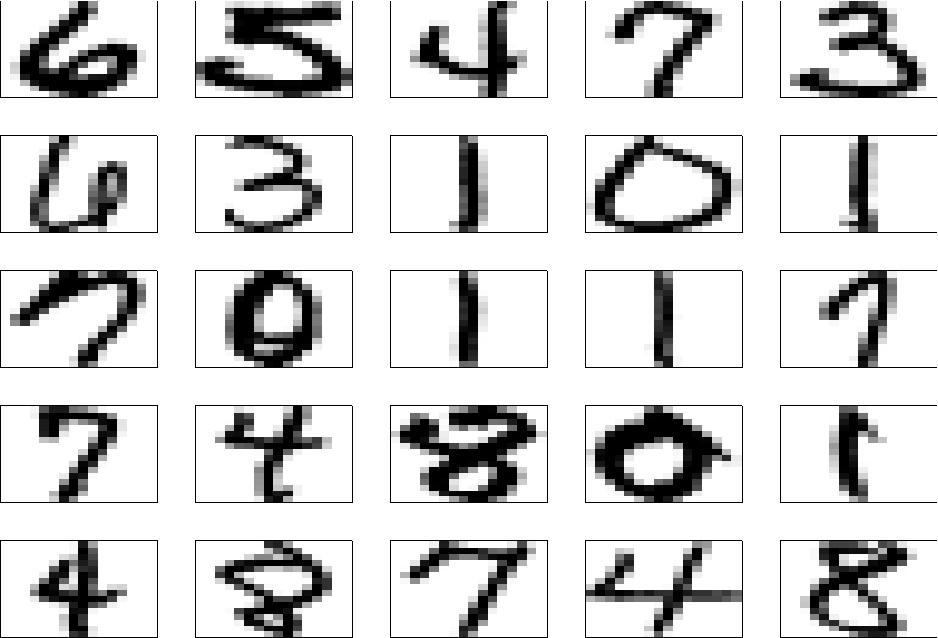
\includegraphics{bookdown-demo_files/figure-latex/25digits-1.pdf}
\caption{\label{fig:25digits}The first 25 handwritten numerals, digitized}
\end{figure}

\begin{figure}
\centering
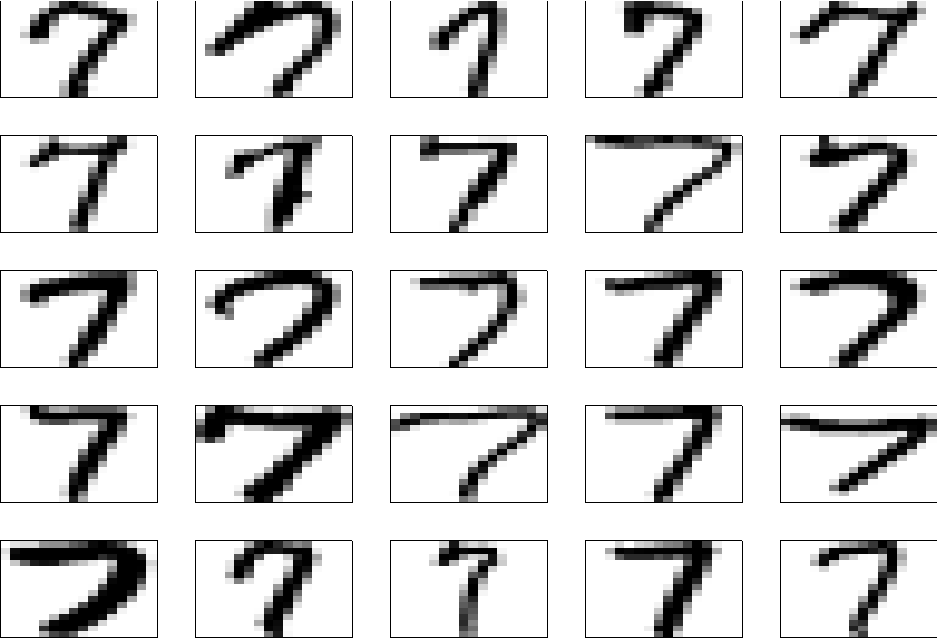
\includegraphics{bookdown-demo_files/figure-latex/25Sevens-1.pdf}
\caption{\label{fig:25Sevens}The first 25 numeral sevens, digitized}
\end{figure}

\section{Looking Forward}\label{looking-forward}

The four examples above illustrate a small sample of the wide variety of
data sets that may be encountered in data science. Each of these
provides its own challenges. The baby crawling data present challenges
that are more statistical in nature. For example, how might the study
design (which isn't described here) affect methods of analysis and
conclusions drawn from the study? Similar challenges are also present
within the other data sets, but these data sets also present more
substantial challenges prior to (and during) the analysis stage, such as
how to work with the missing data in the World Bank data set, or how to
effectively and efficiently process the email data to extract features
of interest.

This book and associated material introduce tools to tackle some of the
challenges in working with real data sets, within the context of the R
statistical system. We will focus on important topics such as

\begin{enumerate}
\def\labelenumi{\arabic{enumi}.}
\tightlist
\item
  Obtaining and manipulating data
\item
  Graphical tools for exploring and summarizing data
\item
  Communicating findings about data that support reproducible research
\item
  Tools for classification problems such as email spam filtering or
  handwritten digit recognition
\item
  Programming and wirting functions in R
\end{enumerate}

\section{How to learn (The most important section in this
book!)}\label{how-to-learn-the-most-important-section-in-this-book}

There are several ways to engage with the content of this book and
associated materials.

One way is not to engage at all. Leave the book closed on a shelf and do
something else with your time. That may or may not be a good life
strategy, depending on what else you do with your time, but you won't
learn much from the book!

Another way to engage is to read through the book ``passively'', reading
all that's written but not reading the book while at your computer,
where you could enter the R commands from the book. With this strategy
you'll probably learn more than if you leave the book closed on a shelf,
but there are better options.

A third way to engage is to read the book while you're at a computer,
enter the R commands from the book as you read about them, and work on
the practice exercises at the end of each chapter. You'll likely learn
more this way.

A fourth strategy is even better. In addition to reading, entering the
commands given in the book, and working through the practice exercises,
you think about what you're doing, and ask yourself questions (which you
then go on to answer). For example after working through some R code
computing the logarithm of positive numbers you might ask yourself,
``What would R do if I asked it to calculate the logarithm of a negative
number? What would R do if I asked it to calculate the logarithm of a
really large number such as one trillion?'' You could explore these
questions easily by just trying things out in the R Console window.

If your goal is to maximize the time you have to binge-watch
\emph{Stranger Things} Season 2 on Netflix, the first strategy may be
optimal. But if your goal is to learn a lot about computational tools
for data science, the fourth strategy is probably going to be best.

\chapter{Introduction to R and
RStudio}\label{introduction-to-r-and-rstudio}

Various statistical and programming software environments are used in
data science, including R, Python, SAS, C++, SPSS, and many others. Each
has strengths and weaknesses, and often two or more are used in a single
project. This book focuses on R for several reasons:

\begin{enumerate}
\def\labelenumi{\arabic{enumi}.}
\tightlist
\item
  R is free
\item
  It is one of, if not the, most widely used software environments in
  data science
\item
  R is under constant and open development by a diverse and expert core
  group
\item
  It has an incredible variety of contributed packages
\item
  A new user can (relatively) quickly gain enough skills to obtain,
  manage, and analyze data in R
\end{enumerate}

Several enhanced interfaces for R have been developed. Generally such
interfaces are referred to as \emph{integrated development environments
(IDE)}. These interfaces are used to facilitate software development. At
minimum, an IDE typically consists of a source code editor and build
automation tools. We will use the RStudio IDE, which according to its
developers ``is a powerful productive user interface for R.''\footnote{\url{http://www.rstudio.com/}}
RStudio is widely used, it is used increasingly in the R community, and
it makes learning to use R a bit simpler. Although we will use RStudio,
most of what is presented in this book can be accomplished in R (without
an added interface) with few or no changes.

\section{Obtaining and Installing R}\label{obtaining-and-installing-r}

It is simple to install R on computers running Microsoft Windows, macOS,
or Linux. For other operating systems users can compile the source code
directly.\footnote{Windows, macOS, and Linux users also can compile the
  source code directly, but for most it is a better idea to install R
  from already compiled binary distributions.} Here is a step-by-step
guide to installing R for Microsoft Windows.\footnote{New versions of R
  are released regularly, so the version number in Step 6 might be
  different from what is listed below.} macOS and Linux users would
follow similar steps.

\begin{enumerate}
\def\labelenumi{\arabic{enumi}.}
\tightlist
\item
  Go to \url{http://www.r-project.org/}
\item
  Click on the \texttt{CRAN} link on the left side of the page
\item
  Choose one of the mirrors.\footnote{The \url{http://cran.rstudio.com/}
    mirror is usually fast. Otherwise choose a mirror in Michigan.}
\item
  Click on \texttt{Download\ R\ for\ Windows}
\item
  Click on \texttt{base}
\item
  Click on \texttt{Download\ R\ 3.5.0\ for\ Windows}
\item
  Install R as you would install any other Windows program
\end{enumerate}

\section{Obtaining and Installing
RStudio}\label{obtaining-and-installing-rstudio}

You must install R prior to installing RStudio. RStudio is also simple
to install:

\begin{enumerate}
\def\labelenumi{\arabic{enumi}.}
\tightlist
\item
  Go to \url{http://www.rstudio.com}
\item
  Click on the link \texttt{RStudio} under the \texttt{Products} tab,
  then select the \texttt{Desktop} option
\item
  Click on the \texttt{Desktop} link
\item
  Choose the \texttt{DOWNLOAD\ RSTUDIO\ DESKTOP} link in the
  \texttt{Open\ Source\ Edition} column
\item
  On the ensuing page, click on the \texttt{Installer} version for your
  operating system, and once downloaded, install as you would any
  program
\end{enumerate}

\section{Using R and RStudio}\label{using-r-and-rstudio}

Start RStudio as you would any other program in your operating system.
For example, under Microsoft Windows use the Start Menu or double click
on the shortcut on the desktop (if a shortcut was created in the
installation process). A (rather small) view of RStudio is displayed in
Figure \ref{fig:rstudioPic}.

\begin{figure}
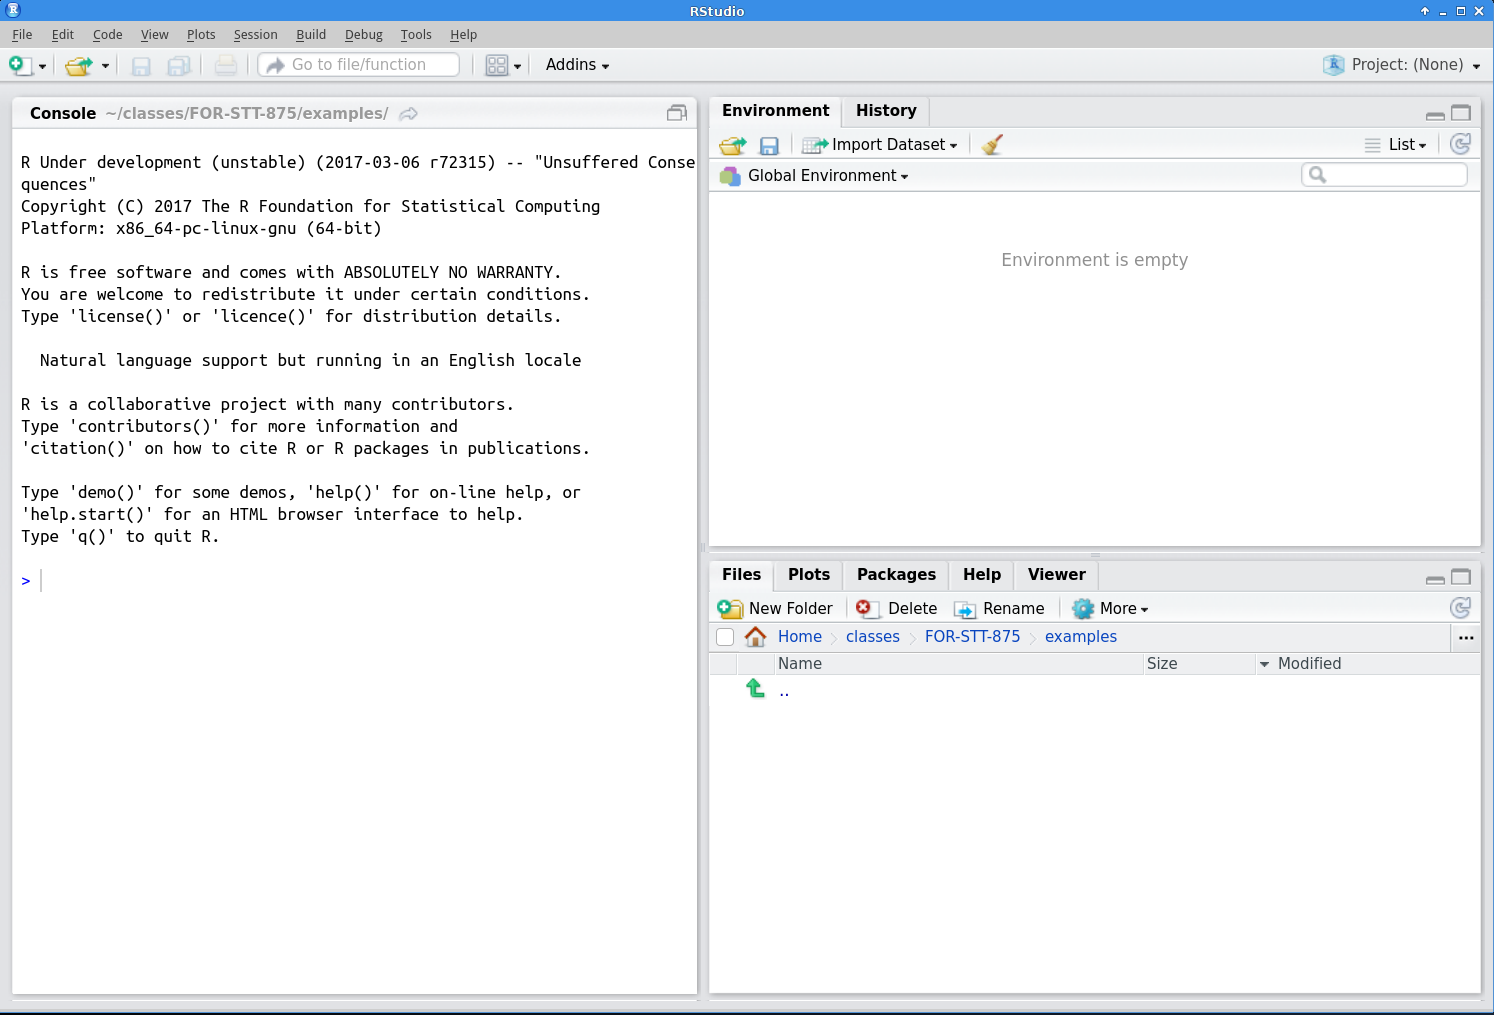
\includegraphics[width=20.75in]{../figures/RStudio} \caption{The RStudio IDE}\label{fig:rstudioPic}
\end{figure}

Initially the RStudio window contains three smaller windows. For now our
main focus will be the large window on the left, the \texttt{Console}
window, in which R statements are typed. The next few sections give
simple examples of the use of R. In these sections we will focus on
small and non-complex data sets, but of course later in the book we will
work with much larger and more complex sets of data. Read these sections
at your computer with R running, and enter the R commands there to get
comfortable using the R console window and RStudio.

\subsection{R as a Calculator}\label{r-as-a-calculator}

R can be used as a calculator. Note that \texttt{\#} is the comment
character in R, so R ignores everything following this character. Also,
you will see that R prints \texttt{{[}1{]}} before the results of each
command. Soon we will explain its relevance, but ignore this for now.
The command prompt in R is the greater than sign
\texttt{\textgreater{}}.

\begin{Shaded}
\begin{Highlighting}[]
\OperatorTok{>}\StringTok{ }\DecValTok{34} \OperatorTok{+}\StringTok{ }\DecValTok{20} \OperatorTok{*}\StringTok{ }\KeywordTok{sqrt}\NormalTok{(}\DecValTok{100}\NormalTok{)  ## +,-,*,/ have the expected meanings}
\end{Highlighting}
\end{Shaded}

\begin{verbatim}
[1] 234
\end{verbatim}

\begin{Shaded}
\begin{Highlighting}[]
\OperatorTok{>}\StringTok{ }\KeywordTok{exp}\NormalTok{(}\DecValTok{2}\NormalTok{)  ##The exponential function}
\end{Highlighting}
\end{Shaded}

\begin{verbatim}
[1] 7.389
\end{verbatim}

\begin{Shaded}
\begin{Highlighting}[]
\OperatorTok{>}\StringTok{ }\KeywordTok{log10}\NormalTok{(}\DecValTok{100}\NormalTok{)  ##Base 10 logarithm}
\end{Highlighting}
\end{Shaded}

\begin{verbatim}
[1] 2
\end{verbatim}

\begin{Shaded}
\begin{Highlighting}[]
\OperatorTok{>}\StringTok{ }\KeywordTok{log}\NormalTok{(}\DecValTok{100}\NormalTok{)  ##Base e logarithm}
\end{Highlighting}
\end{Shaded}

\begin{verbatim}
[1] 4.605
\end{verbatim}

\begin{Shaded}
\begin{Highlighting}[]
\OperatorTok{>}\StringTok{ }\DecValTok{10}\OperatorTok{^}\KeywordTok{log10}\NormalTok{(}\DecValTok{55}\NormalTok{)}
\end{Highlighting}
\end{Shaded}

\begin{verbatim}
[1] 55
\end{verbatim}

Most functions in R can be applied to vector arguments rather than
operating on a single argument at a time. A \texttt{vector} is a data
structure that contains elements of the same data type (i.e.~integers).

\begin{Shaded}
\begin{Highlighting}[]
\OperatorTok{>}\StringTok{ }\DecValTok{1}\OperatorTok{:}\DecValTok{25}\NormalTok{  ##The integers from 1 to 25}
\end{Highlighting}
\end{Shaded}

\begin{verbatim}
 [1]  1  2  3  4  5  6  7  8  9 10 11 12 13 14 15 16 17
[18] 18 19 20 21 22 23 24 25
\end{verbatim}

\begin{Shaded}
\begin{Highlighting}[]
\OperatorTok{>}\StringTok{ }\KeywordTok{log}\NormalTok{(}\DecValTok{1}\OperatorTok{:}\DecValTok{25}\NormalTok{)  ##The base e logarithm of these integers}
\end{Highlighting}
\end{Shaded}

\begin{verbatim}
 [1] 0.0000 0.6931 1.0986 1.3863 1.6094 1.7918 1.9459
 [8] 2.0794 2.1972 2.3026 2.3979 2.4849 2.5649 2.6391
[15] 2.7081 2.7726 2.8332 2.8904 2.9444 2.9957 3.0445
[22] 3.0910 3.1355 3.1781 3.2189
\end{verbatim}

\begin{Shaded}
\begin{Highlighting}[]
\OperatorTok{>}\StringTok{ }\DecValTok{1}\OperatorTok{:}\DecValTok{25} \OperatorTok{*}\StringTok{ }\DecValTok{1}\OperatorTok{:}\DecValTok{25}\NormalTok{  ##What will this produce?}
\end{Highlighting}
\end{Shaded}

\begin{verbatim}
 [1]   1   4   9  16  25  36  49  64  81 100 121 144
[13] 169 196 225 256 289 324 361 400 441 484 529 576
[25] 625
\end{verbatim}

\begin{Shaded}
\begin{Highlighting}[]
\OperatorTok{>}\StringTok{ }\DecValTok{1}\OperatorTok{:}\DecValTok{25} \OperatorTok{*}\StringTok{ }\DecValTok{1}\OperatorTok{:}\DecValTok{5}\NormalTok{  ##What about this?}
\end{Highlighting}
\end{Shaded}

\begin{verbatim}
 [1]   1   4   9  16  25   6  14  24  36  50  11  24
[13]  39  56  75  16  34  54  76 100  21  44  69  96
[25] 125
\end{verbatim}

\begin{Shaded}
\begin{Highlighting}[]
\OperatorTok{>}\StringTok{ }\KeywordTok{seq}\NormalTok{(}\DataTypeTok{from =} \DecValTok{0}\NormalTok{, }\DataTypeTok{to =} \DecValTok{1}\NormalTok{, }\DataTypeTok{by =} \FloatTok{0.1}\NormalTok{)  ##A sequence of numbers from 0 to 1}
\end{Highlighting}
\end{Shaded}

\begin{verbatim}
 [1] 0.0 0.1 0.2 0.3 0.4 0.5 0.6 0.7 0.8 0.9 1.0
\end{verbatim}

\begin{Shaded}
\begin{Highlighting}[]
\OperatorTok{>}\StringTok{ }\KeywordTok{exp}\NormalTok{(}\KeywordTok{seq}\NormalTok{(}\DataTypeTok{from =} \DecValTok{0}\NormalTok{, }\DataTypeTok{to =} \DecValTok{1}\NormalTok{, }\DataTypeTok{by =} \FloatTok{0.1}\NormalTok{))  ##What will this produce?}
\end{Highlighting}
\end{Shaded}

\begin{verbatim}
 [1] 1.000 1.105 1.221 1.350 1.492 1.649 1.822 2.014
 [9] 2.226 2.460 2.718
\end{verbatim}

Now the mysterious square bracketed numbers appearing next to the output
make sense. R puts the position of the beginning value on a line in
square brackets before the line of output. For example if the output has
40 values, and 15 values appear on each line, then the first line will
have \texttt{{[}1{]}} at the left, the second line will have
\texttt{{[}16{]}} to the left, and the third line will have
\texttt{{[}31{]}} to the left.

\subsection{Basic descriptive statistics and graphics in R}\label{dec}

It is easy to compute basic descriptive statistics and to produce
standard graphical representations of data in R. First we create three
variables with horsepower, miles per gallon, and names for 15
cars.\footnote{These are from a relatively old data set, with 1974 model
  cars.} In this case with a small data set we enter the data ``by
hand'' using the \texttt{c()} function, which concatenates its arguments
into a vector. For larger data sets we will clearly want an alternative.
Note that character values are surrounded by quotation marks.

A style note: R has two widely used methods of assignment: the left
arrow, which consists of a less than sign followed immediately by a
dash: \texttt{\textless{}-} and the equals sign: \texttt{=}. Much ink
has been used debating the relative merits of the two methods, and their
subtle differences. Many leading R style guides (e.g., the Google style
guide at \url{https://google.github.io/styleguide/Rguide.xml} and the
Bioconductor style guide at
\url{http://www.bioconductor.org/developers/how-to/coding-style/})
recommend the left arrow \texttt{\textless{}-} as an assignment
operator, and we will use this throughout the book.

Also you will see that if a command has not been completed but the ENTER
key is pressed, the command prompt changes to a \texttt{+} sign.

\begin{Shaded}
\begin{Highlighting}[]
\OperatorTok{>}\StringTok{ }\NormalTok{car.hp <-}\StringTok{ }\KeywordTok{c}\NormalTok{(}\DecValTok{110}\NormalTok{, }\DecValTok{110}\NormalTok{, }\DecValTok{93}\NormalTok{, }\DecValTok{110}\NormalTok{, }\DecValTok{175}\NormalTok{, }\DecValTok{105}\NormalTok{, }\DecValTok{245}\NormalTok{, }\DecValTok{62}\NormalTok{, }\DecValTok{95}\NormalTok{, }\DecValTok{123}\NormalTok{, }
\OperatorTok{+}\StringTok{ }\DecValTok{123}\NormalTok{, }\DecValTok{180}\NormalTok{, }\DecValTok{180}\NormalTok{, }\DecValTok{180}\NormalTok{, }\DecValTok{205}\NormalTok{)}
\OperatorTok{>}\StringTok{ }\NormalTok{car.mpg <-}\StringTok{ }\KeywordTok{c}\NormalTok{(}\FloatTok{21.0}\NormalTok{, }\FloatTok{21.0}\NormalTok{, }\FloatTok{22.8}\NormalTok{, }\FloatTok{21.4}\NormalTok{, }\FloatTok{18.7}\NormalTok{, }\FloatTok{18.1}\NormalTok{, }\FloatTok{14.3}\NormalTok{, }\FloatTok{24.4}\NormalTok{, }\FloatTok{22.8}\NormalTok{, }
\OperatorTok{+}\StringTok{              }\FloatTok{19.2}\NormalTok{, }\FloatTok{17.8}\NormalTok{, }\FloatTok{16.4}\NormalTok{, }\FloatTok{17.3}\NormalTok{, }\FloatTok{15.2}\NormalTok{, }\FloatTok{10.4}\NormalTok{)}
\OperatorTok{>}\StringTok{ }\NormalTok{car.name <-}\StringTok{ }\KeywordTok{c}\NormalTok{(}\StringTok{"Mazda RX4"}\NormalTok{, }\StringTok{"Mazda RX4 Wag"}\NormalTok{, }\StringTok{"Datsun 710"}\NormalTok{, }
\OperatorTok{+}\StringTok{               "Hornet 4 Drive"}\NormalTok{, }\StringTok{"Hornet Sportabout"}\NormalTok{, }\StringTok{"Valiant"}\NormalTok{, }
\OperatorTok{+}\StringTok{               "Duster 360"}\NormalTok{, }\StringTok{"Merc 240D"}\NormalTok{, }\StringTok{"Merc 230"}\NormalTok{, }\StringTok{"Merc 280"}\NormalTok{, }
\OperatorTok{+}\StringTok{               "Merc 280C"}\NormalTok{, }\StringTok{"Merc 450SE"}\NormalTok{, }\StringTok{"Merc 450SL"}\NormalTok{, }
\OperatorTok{+}\StringTok{               "Merc 450SLC"}\NormalTok{, }\StringTok{"Cadillac Fleetwood"}\NormalTok{)}
\OperatorTok{>}\StringTok{ }\NormalTok{car.hp}
\end{Highlighting}
\end{Shaded}

\begin{verbatim}
 [1] 110 110  93 110 175 105 245  62  95 123 123 180
[13] 180 180 205
\end{verbatim}

\begin{Shaded}
\begin{Highlighting}[]
\OperatorTok{>}\StringTok{ }\NormalTok{car.mpg}
\end{Highlighting}
\end{Shaded}

\begin{verbatim}
 [1] 21.0 21.0 22.8 21.4 18.7 18.1 14.3 24.4 22.8 19.2
[11] 17.8 16.4 17.3 15.2 10.4
\end{verbatim}

\begin{Shaded}
\begin{Highlighting}[]
\OperatorTok{>}\StringTok{ }\NormalTok{car.name}
\end{Highlighting}
\end{Shaded}

\begin{verbatim}
 [1] "Mazda RX4"          "Mazda RX4 Wag"     
 [3] "Datsun 710"         "Hornet 4 Drive"    
 [5] "Hornet Sportabout"  "Valiant"           
 [7] "Duster 360"         "Merc 240D"         
 [9] "Merc 230"           "Merc 280"          
[11] "Merc 280C"          "Merc 450SE"        
[13] "Merc 450SL"         "Merc 450SLC"       
[15] "Cadillac Fleetwood"
\end{verbatim}

Next we compute some descriptive statistics for the two numeric
variables (\texttt{car.hp} and \texttt{car.mpg})

\begin{Shaded}
\begin{Highlighting}[]
\OperatorTok{>}\StringTok{ }\KeywordTok{mean}\NormalTok{(car.hp)}
\end{Highlighting}
\end{Shaded}

\begin{verbatim}
[1] 139.7
\end{verbatim}

\begin{Shaded}
\begin{Highlighting}[]
\OperatorTok{>}\StringTok{ }\KeywordTok{sd}\NormalTok{(car.hp)}
\end{Highlighting}
\end{Shaded}

\begin{verbatim}
[1] 50.78
\end{verbatim}

\begin{Shaded}
\begin{Highlighting}[]
\OperatorTok{>}\StringTok{ }\KeywordTok{summary}\NormalTok{(car.hp)}
\end{Highlighting}
\end{Shaded}

\begin{verbatim}
   Min. 1st Qu.  Median    Mean 3rd Qu.    Max. 
     62     108     123     140     180     245 
\end{verbatim}

\begin{Shaded}
\begin{Highlighting}[]
\OperatorTok{>}\StringTok{ }\KeywordTok{mean}\NormalTok{(car.mpg)}
\end{Highlighting}
\end{Shaded}

\begin{verbatim}
[1] 18.72
\end{verbatim}

\begin{Shaded}
\begin{Highlighting}[]
\OperatorTok{>}\StringTok{ }\KeywordTok{sd}\NormalTok{(car.mpg)}
\end{Highlighting}
\end{Shaded}

\begin{verbatim}
[1] 3.714
\end{verbatim}

\begin{Shaded}
\begin{Highlighting}[]
\OperatorTok{>}\StringTok{ }\KeywordTok{summary}\NormalTok{(car.mpg)}
\end{Highlighting}
\end{Shaded}

\begin{verbatim}
   Min. 1st Qu.  Median    Mean 3rd Qu.    Max. 
   10.4    16.9    18.7    18.7    21.2    24.4 
\end{verbatim}

Next, a scatter plot of \texttt{cars.mpg} versus \texttt{cars.hp}:

\begin{Shaded}
\begin{Highlighting}[]
\OperatorTok{>}\StringTok{ }\KeywordTok{plot}\NormalTok{(car.hp, car.mpg)}
\end{Highlighting}
\end{Shaded}

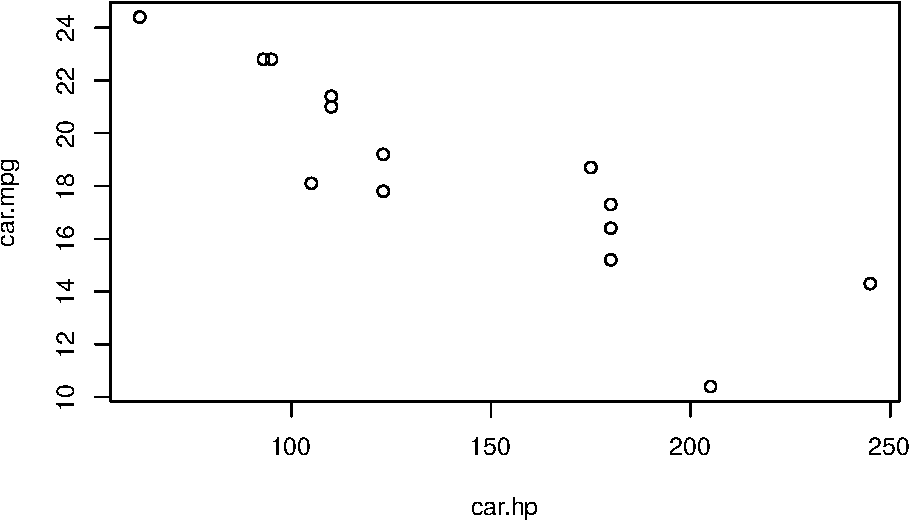
\includegraphics{bookdown-demo_files/figure-latex/unnamed-chunk-8-1.pdf}

Unsurprisingly as horsepower increases, mpg tends to decrease. This
relationship can be investigated further using linear regression, a
statistical procedure that involves fitting a linear model to a data set
in order to further understand the relationship between two variables.

\subsection{An Initial Tour of
RStudio}\label{an-initial-tour-of-rstudio}

When you created the \texttt{car.hp} and other vectors in the previous
section, you might have noticed the vector name and a short description
of its attributes appear in the top right \texttt{Global\ Environment}
window. Similarly, when you called \texttt{plot(car.hp,car.mpg)} the
corresponding plot appeared in the lower right \texttt{Plots} window.

A comprehensive, but slightly overwhelming, cheatsheet for RStudio is
available here
\url{https://www.rstudio.com/wp-content/uploads/2016/01/rstudio-IDE-cheatsheet.pdf}.
As we progress in learning R and RStudio, this cheatsheet will become
more useful. For now you might use the cheatsheet to locate the various
windows and functions identified in the coming chapters.

\section{Getting Help}\label{getting-help}

There are several free (and several not free) ways to get R help when
needed.

Several help-related functions are built into R. If there's a particular
R function of interest, such as \texttt{log}, \texttt{help(log)} or
\texttt{?log} will bring up a help page for that function. In RStudio
the help page is displayed, by default, in the \texttt{Help} tab in the
lower right window.\footnote{There are ways to change this default
  behavior.} The function \texttt{help.start} opens a window which
allows browsing of the online documentation included with R. To use
this, type \texttt{help.start()} in the console window.\footnote{You may
  wonder about the parentheses after \texttt{help.start}. A user can
  specify arguments to any R function inside parentheses. For example
  \texttt{log(10)} asks R to return the logarithm of the argument 10.
  Even if no arguments are needed, R requires empty parentheses at the
  end of any function name. In fact if you just type the function name
  without parentheses, R returns the definition of the function. For
  simple functions this can be illuminating.} The \texttt{help.start}
function also provides several manuals online and can be a useful
interface in addition to the built in help.

Search engines provide another, sometimes more user-friendly, way to
receive answers for R questions. A Google search often quickly finds
something written by another user who had the same (or a similar)
question, or an online tutorial that touches on the question. More
specialized is \href{http://rseek.org}{rseek.org}, which is a search
engine focused specifically on R. Both Google and
\href{http://rseek.org}{rseek.org} are valuable tools, often providing
more user-friendly information then R's own help system.

In addition, R users have written many types of contributed
documentation. Some of this documentation is available at
\url{http://cran.r-project.org/other-docs.html}. Of course there are
also numerous books covering general and specialized R topics available
for purchase.

\section{Workspace, Working Directory, and Keeping
Organized}\label{workspace-working-directory-and-keeping-organized}

The \emph{workspace} is your R session working environment and includes
any objects you create. Recall these objects are listed in the
\texttt{Global\ Environment} window. The command \texttt{ls()}, which
stands for list, will also list all the objects in your workspace (note,
this is the same list that is given in the \texttt{Global\ Environment}
window). When you close RStudio, a dialog box will ask you if you want
to save an image of the current workspace. If you choose to save your
workspace, RStudio saves your session objects and information in a
\texttt{.RData} file (the period makes it a hidden file) in your
\emph{working directory}. Next time you start R or RStudio it checks if
there is a \texttt{.RData} in the working directory, loads it if it
exists, and your session continues where you left off. Otherwise R
starts with an empty workspace. This leads to the next question---what
is a working directory?

Each R session is associated with a working directory. This is just a
directory from which R reads and writes files, e.g., the \texttt{.RData}
file, data files you want to analyze, or files you want to save. On Mac
when you start RStudio it sets the working directory to your home
directory (for me that's \texttt{/Users/andy}). If you're on a different
operating system, you can check where the default working directory is
by typing \texttt{getwd()} in the console. You can change the default
working directory under RStudio's \verb+Global Option+ dialog found
under the \texttt{Tools} dropdown menu. There are multiple ways to
change the working directory once an R session is started in RStudio.
One method is to click on the \texttt{Files} tab in the lower right
window and then click the \texttt{More} button. Alternatively, you can
set the session's working directory using the \texttt{setwd()} in the
console. For example, on Windows
\texttt{setwd("C:/Users/andy/for875/exercise1")} will set the working
directory to \texttt{C:/Users/andy/for875/exercise1}, assuming that file
path and directory exist (Note: Windows file path uses a backslash,
\texttt{\textbackslash{}}, but in R the backslash is an escape
character, hence specifying file paths in R on Windows uses the forward
slash, i.e., \texttt{/}). Similarly on Mac you can use
\texttt{setwd("/Users/andy/for875/exercise1")}. Perhaps the most simple
method is to click on the \texttt{Session} tab at the top of your screen
and click on the \texttt{Set\ Working\ Directory} option. Later on when
we start reading and writing data from our R session, it will be very
important that you are able to identify your current working directory
and change it if needed. We will revisit this in subsequent chapters.

As with all work, keeping organized is the key to efficiency. It is good
practice to have a dedicated directory for each R project or exercise.

\section{Quality of R code}\label{quality-of-r-code}

\begin{figure}
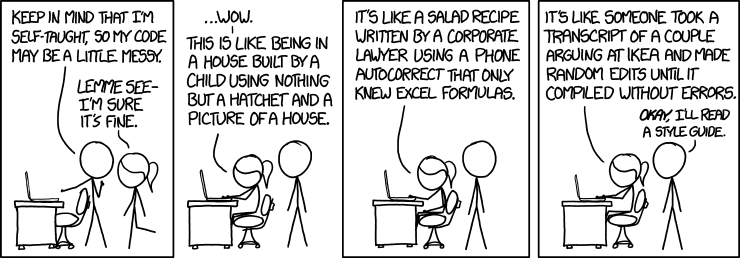
\includegraphics[width=10.28in]{../figures/code_quality} \caption{Code Quality}\label{fig:comic}
\end{figure}

Writing well-organized and well-labeled code allows your code to be more
easily read and understood by another person. (See xkcd's take on code
quality in Figure \ref{fig:comic}.) More importantly, though, your
well-written code is more accessible to you hours, days, or even months
later. We are hoping that you can use the code you write in this class
in future projects and research.

Google provides style guides for many programming languages. You can
find the R style guide
\href{https://google.github.io/styleguide/Rguide.xml}{here}. Below are a
few of the key points from the guide that we will use right away.

\subsection{Naming Files}\label{naming-files}

File names should be meaningful and end in \texttt{.R}. If we write a
script that analyzes a certain species distribution:

\begin{itemize}
\tightlist
\item
  GOOD: \(\color{green}{\verb+african_rhino_distribution.R+}\)
\item
  GOOD: \(\color{green}{\verb+africanRhinoDistribution.R+}\)
\item
  BAD: \(\color{red}{\verb+speciesDist.R+}\) (too ambiguous)
\item
  BAD: \(\color{red}{\verb+species.dist.R+}\) (too ambiguous and two
  periods can confuse operating systems' file type auto-detect)
\item
  BAD: \(\color{red}{\verb+speciesdist.R+}\) (too ambiguous and
  confusing)
\end{itemize}

\subsection{Naming Variables}\label{naming-variables}

\begin{itemize}
\tightlist
\item
  GOOD: \(\color{green}{\verb+rhino.count+}\)
\item
  GOOD: \(\color{green}{\verb+rhinoCount+}\)
\item
  GOOD: \(\color{green}{\verb+rhino_count+}\) (We don't mind the
  underscore and use it quite often, although Google's style guide says
  it's a no-no for some reason)
\item
  BAD: \(\color{red}{\verb+rhinocount+}\) (confusing)
\end{itemize}

\subsection{Syntax}\label{syntax}

\begin{itemize}
\tightlist
\item
  Keep code lines under 80 characters long.
\item
  Indent your code with two spaces. (RStudio does this by default when
  you press the TAB key.)
\end{itemize}

\chapter{Scripts and R Markdown}\label{scripts-and-r-markdown}

Doing work in data science, whether for homework, a project for a
business, or a research project, typically involves several iterations.
For example creating an effective graphical representation of data can
involve trying out several different graphical representations, and then
tens if not hundreds of iterations when fine-tuning the chosen
representation. Furthermore, each of these representations may require
several R commands to create. Although this all could be accomplished by
typing and re-typing commands at the R Console, it is easier and more
effective to write the commands in a \emph{script file}, which then can
be submitted to the R console either a line at a time or all
together.\footnote{Unsurprisingly it is also possible to submit several
  selected lines of code at once.}

In addition to making the workflow more efficient, R scripts provide
another large benefit. Often we work on one part of a homework
assignment or project for a few hours, then move on to something else,
and then return to the original part a few days, months, or sometimes
even years later. In such cases we may have forgotten how we created the
graphical display that we were so proud of, and will need to again spend
a few hours to recreate it. If we save a script file, we have the
ingredients immediately available when we return to a portion of a
project.\footnote{In principle the R history mechanism provides a
  similar record. But with history we have to search through a lot of
  other code to find what we're looking for, and scripts are a much
  cleaner mechanism to record our work.}

Next consider the larger scientific endeavor. Ideally a scientific study
will be reproducible, meaning that an independent group of researchers
(or the original researchers) will be able to duplicate the study.
Thinking about data science, this means that all the steps taken when
working with the data from a study should be reproducible, from the
selection of variables to formal data analysis. In principle, this can
be facilitated by explaining, in words, each step of the work with data.
In practice, it is typically difficult or impossible to reproduce a full
data analysis based on a written explanation. Much more effective is to
include the actual computer code which accomplished the data work in the
report, whether the report is a homework assignment or a research paper.
Tools in R such as \emph{R Markdown} facilitate this process.

\section{Scripts in R}\label{scripts-in-r}

As noted above, scripts help to make work with data more efficient and
provide a record of how data were managed and analyzed. Below we
describe an example. This example uses features of R that we have not
yet discussed, so don't worry about the details, but rather about how it
motivates the use of a script file.

First we read in a data set containing data on (among other things)
fertility rate and life expectancy for countries throughout the world,
for the years 1960 through 2014.

\begin{Shaded}
\begin{Highlighting}[]
\OperatorTok{>}\StringTok{ }\NormalTok{u <-}\StringTok{ "http://blue.for.msu.edu/FOR875/data/WorldBank.csv"}
\OperatorTok{>}\StringTok{ }\NormalTok{WorldBank <-}\StringTok{ }\KeywordTok{read.csv}\NormalTok{(u, }\DataTypeTok{header =} \OtherTok{TRUE}\NormalTok{, }\DataTypeTok{stringsAsFactors =} \OtherTok{FALSE}\NormalTok{)}
\end{Highlighting}
\end{Shaded}

Next we print the names of the variables in the data set. Don't be
concerned about the specific details. Later we will learn much more
about reading in data and working with data sets in R.

\begin{Shaded}
\begin{Highlighting}[]
\OperatorTok{>}\StringTok{ }\KeywordTok{names}\NormalTok{(WorldBank)}
\end{Highlighting}
\end{Shaded}

\begin{verbatim}
 [1] "iso2c"                       
 [2] "country"                     
 [3] "year"                        
 [4] "fertility.rate"              
 [5] "life.expectancy"             
 [6] "population"                  
 [7] "GDP.per.capita.Current.USD"  
 [8] "X15.to.25.yr.female.literacy"
 [9] "iso3c"                       
[10] "region"                      
[11] "capital"                     
[12] "longitude"                   
[13] "latitude"                    
[14] "income"                      
[15] "lending"                     
\end{verbatim}

We will try to create a scatter plot of fertility rate versus life
expectancy of countries for the year 1960. To do this we'll first create
variables containing the values of fertility rate and life expectancy
for 1960\footnote{This isn't necessary, but it is convenient}, and print
out the first ten values of each variable.

\begin{Shaded}
\begin{Highlighting}[]
\OperatorTok{>}\StringTok{ }\NormalTok{fertility <-}\StringTok{ }\NormalTok{WorldBank}\OperatorTok{$}\NormalTok{fertility.rate[WorldBank}\OperatorTok{$}\NormalTok{year }\OperatorTok{==}\StringTok{ }
\OperatorTok{+}\StringTok{   }\DecValTok{1960}\NormalTok{]}
\OperatorTok{>}\StringTok{ }\NormalTok{lifeexp <-}\StringTok{ }\NormalTok{WorldBank}\OperatorTok{$}\NormalTok{life.expectancy[WorldBank}\OperatorTok{$}\NormalTok{year }\OperatorTok{==}\StringTok{ }\DecValTok{1960}\NormalTok{]}
\OperatorTok{>}\StringTok{ }\NormalTok{fertility[}\DecValTok{1}\OperatorTok{:}\DecValTok{10}\NormalTok{]}
\end{Highlighting}
\end{Shaded}

\begin{verbatim}
 [1]    NA 6.928 7.671 4.425 6.186 4.550 7.316 3.109
 [9]    NA 2.690
\end{verbatim}

\begin{Shaded}
\begin{Highlighting}[]
\OperatorTok{>}\StringTok{ }\NormalTok{lifeexp[}\DecValTok{1}\OperatorTok{:}\DecValTok{10}\NormalTok{]}
\end{Highlighting}
\end{Shaded}

\begin{verbatim}
 [1]    NA 52.24 31.58 61.78 62.25 65.86 32.98 65.22
 [9]    NA 68.59
\end{verbatim}

We see that some countries do not have data for 1960. R represents
missing data via \texttt{NA}. Of course at some point it would be good
to investigate which countries' data are missing and why. The
\texttt{plot()} function in R will just omit missing values, and for now
we will just plot the non-missing data. A scatter plot of the data is
drawn next.

\begin{Shaded}
\begin{Highlighting}[]
\OperatorTok{>}\StringTok{ }\KeywordTok{plot}\NormalTok{(lifeexp, fertility)}
\end{Highlighting}
\end{Shaded}

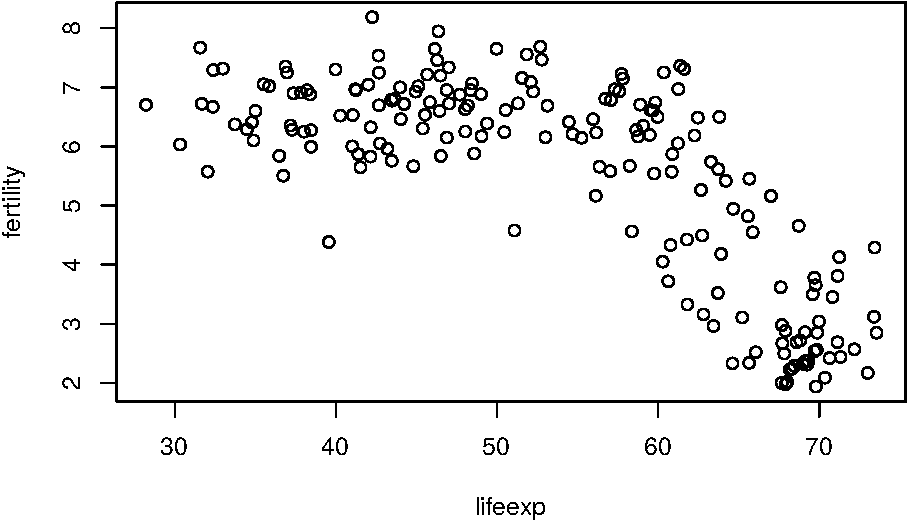
\includegraphics{bookdown-demo_files/figure-latex/unnamed-chunk-12-1.pdf}

The scatter plot shows that as life expectancy increases, fertility rate
tends to decrease in what appears to be a nonlinear relationship. Now
that we have a basic scatter plot, it is tempting to make it more
informative. We will do this by adding two features. One is to make the
points' size proportional to the country's population, and the second is
to make the points' color represent the region of the world the country
resides in. We'll first extract the population and region variables for
1960.

\begin{Shaded}
\begin{Highlighting}[]
\OperatorTok{>}\StringTok{ }\NormalTok{pop <-}\StringTok{ }\NormalTok{WorldBank}\OperatorTok{$}\NormalTok{population[WorldBank}\OperatorTok{$}\NormalTok{year }\OperatorTok{==}\StringTok{ }\DecValTok{1960}\NormalTok{]}
\OperatorTok{>}\StringTok{ }\NormalTok{region <-}\StringTok{ }\NormalTok{WorldBank}\OperatorTok{$}\NormalTok{region[WorldBank}\OperatorTok{$}\NormalTok{year }\OperatorTok{==}\StringTok{ }\DecValTok{1960}\NormalTok{]}
\OperatorTok{>}\StringTok{ }\NormalTok{pop[}\DecValTok{1}\OperatorTok{:}\DecValTok{10}\NormalTok{]}
\end{Highlighting}
\end{Shaded}

\begin{verbatim}
 [1]    13414    89608  8774440    54681  1608800
 [6]  1867396  4965988 20623998    20012  7047539
\end{verbatim}

\begin{Shaded}
\begin{Highlighting}[]
\OperatorTok{>}\StringTok{ }\NormalTok{region[}\DecValTok{1}\OperatorTok{:}\DecValTok{10}\NormalTok{]}
\end{Highlighting}
\end{Shaded}

\begin{verbatim}
 [1] "Europe & Central Asia (all income levels)"     
 [2] "Middle East & North Africa (all income levels)"
 [3] "South Asia"                                    
 [4] "Latin America & Caribbean (all income levels)" 
 [5] "Europe & Central Asia (all income levels)"     
 [6] "Europe & Central Asia (all income levels)"     
 [7] "Sub-Saharan Africa (all income levels)"        
 [8] "Latin America & Caribbean (all income levels)" 
 [9] "East Asia & Pacific (all income levels)"       
[10] "Europe & Central Asia (all income levels)"     
\end{verbatim}

To create the scatter plot we will do two things. First we will create
the axes, labels, etc. for the plot, but not plot the points. The
argument \texttt{type="n"} tells R to do this. Then we will use the
\texttt{symbols()} function to add symbols, the \texttt{circles}
argument to set the sizes of the points, and the \texttt{bg} argument to
set the colors. Don't worry about the details! In fact, later in the
book we will learn about an R package called \texttt{ggplot2} that
provides a different way to create such plots. You'll see two plots
below, first the ``empty'' plot which is just a building block, then the
plot including the appropriate symbols.

\begin{Shaded}
\begin{Highlighting}[]
\OperatorTok{>}\StringTok{ }\KeywordTok{plot}\NormalTok{(lifeexp, fertility, }\DataTypeTok{type=}\StringTok{"n"}\NormalTok{)}
\end{Highlighting}
\end{Shaded}

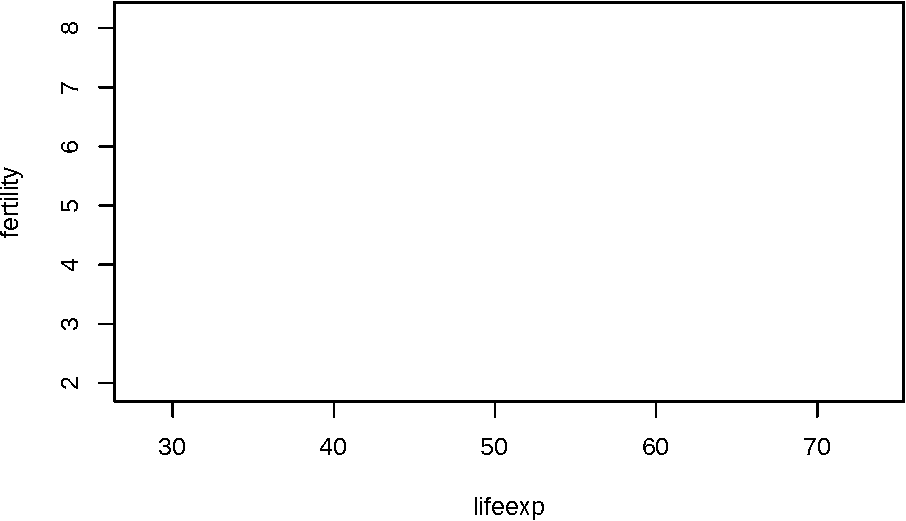
\includegraphics{bookdown-demo_files/figure-latex/unnamed-chunk-14-1.pdf}

\begin{Shaded}
\begin{Highlighting}[]
\OperatorTok{>}\StringTok{ }\KeywordTok{symbols}\NormalTok{(lifeexp, fertility, }\DataTypeTok{circles=}\KeywordTok{sqrt}\NormalTok{(pop}\OperatorTok{/}\NormalTok{pi), }\DataTypeTok{inches=}\FloatTok{0.35}\NormalTok{, }
\OperatorTok{+}\StringTok{         }\DataTypeTok{bg=}\KeywordTok{match}\NormalTok{(region, }\KeywordTok{unique}\NormalTok{(region)))}
\end{Highlighting}
\end{Shaded}

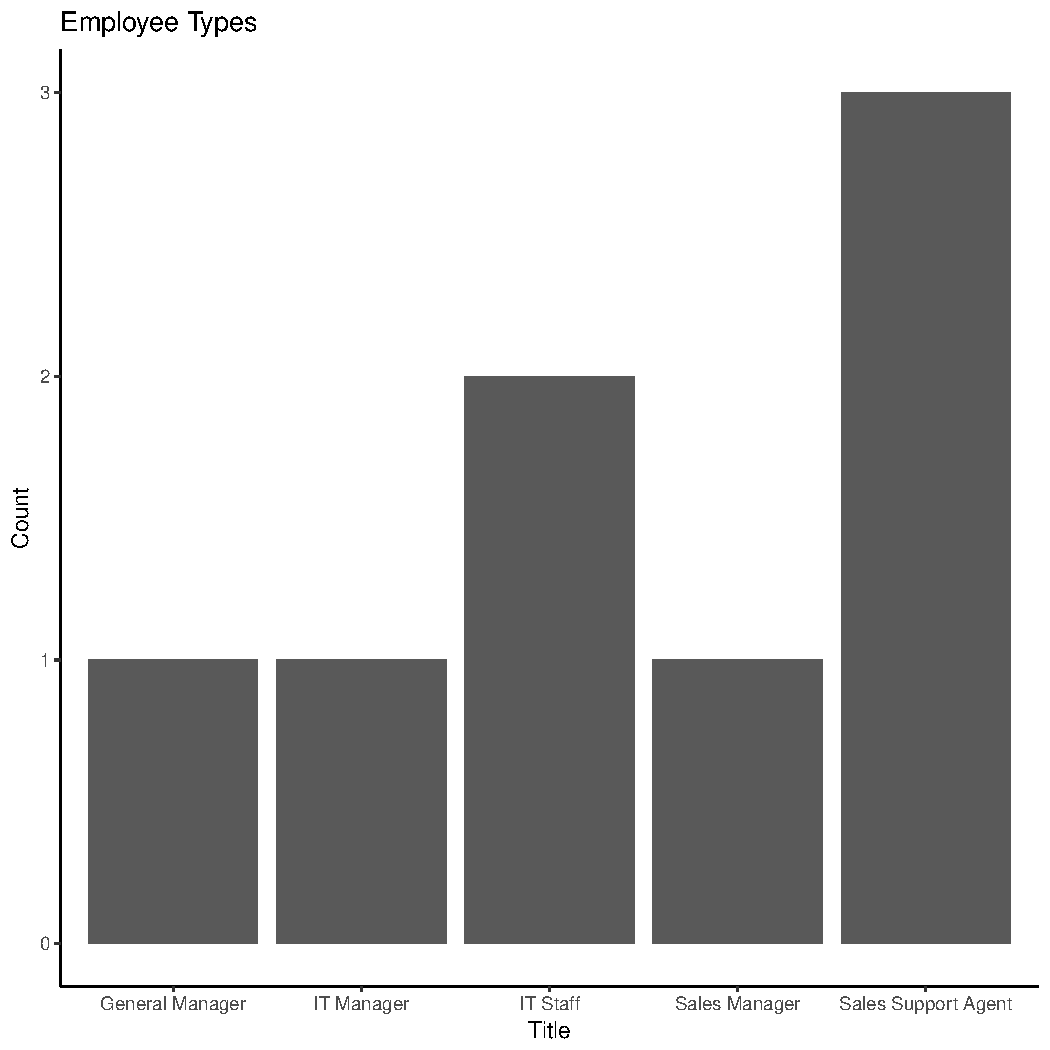
\includegraphics{bookdown-demo_files/figure-latex/unnamed-chunk-14-2.pdf}

Of course we should have a key which tells the viewer which region each
color represents, and a way to determine which country each point
represents, and a lot of other refinements. For now we will resist such
temptations.

Some of the process leading to the completed plot is shown above, such
as reading in the data, creating variables representing the 1960
fertility rate and life expectancy, an intermediate plot that was
rejected, and so on. A lot of the process isn't shown, simply to save
space. There would likely be mistakes (either minor typing mistakes or
more complex errors). Focusing only on the \texttt{symbols()} function
that was used to add the colorful symbols to the scatter plot, there
would likely have been a substantial number of attempts with different
values of the \texttt{circles}, \texttt{inches}, and \texttt{bg}
arguments before settling on the actual form used to create the plot.
This is the typical process you will soon discover when producing useful
data visualizations.

Now imagine trying to recreate the plot a few days later. Possibly
someone saw the plot and commented that it would be interesting to see
some similar plots, but for years in the 1970s when there were major
famines in different countries of the world. If all the work, including
all the false starts and refinements, were done at the console, it would
be hard to sort things out and would take longer than necessary to
create the new plots. This would be especially true if a few months had
passed rather than just a few days.

But with a script file, especially a script file with a few well-chosen
comments, creating the new scatter plots would be much easier.
Fortunately it is quite easy to create and work with script files in
RStudio.\footnote{It is also easy in R without RStudio. Just use
  \texttt{File\ \textgreater{}\ New\ script} to create a script file,
  and save it before exiting R.} Just choose
\texttt{File\ \textgreater{}\ New\ File\ \textgreater{}\ R\ script} and
a script window will open up in the upper left of the full RStudio
window.

An example of a script window (with some R code already typed in) is
shown in Figure \ref{fig:script}. From the script window the user can,
among other things, save the script (either using the \texttt{File} menu
or the icon near the top left of the window) and run one or more lines
of code from the window (using the \texttt{run} icon in the window, or
by copying and pasting into the console window). In addition, there is a
\texttt{Source\ on\ Save} checkbox. If this is checked, the R code in
the script window is automatically read into R and executed when the
script file is saved.

\begin{Shaded}
\begin{Highlighting}[]
\OperatorTok{>}\StringTok{ }\NormalTok{knitr}\OperatorTok{::}\KeywordTok{include_graphics}\NormalTok{(}\StringTok{"../figures/ScriptWindow.PNG"}\NormalTok{)}
\end{Highlighting}
\end{Shaded}

\begin{figure}
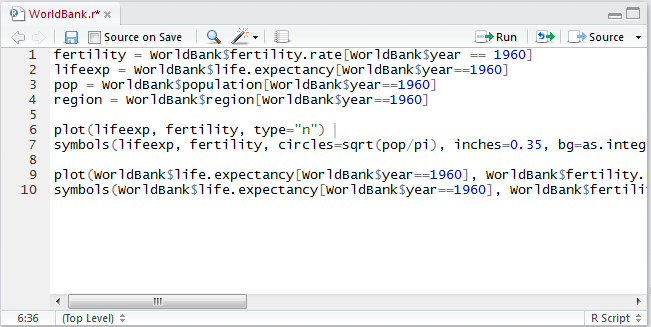
\includegraphics[width=9.04in]{../figures/ScriptWindow} \caption{A script window in RStudio}\label{fig:script}
\end{figure}

\section{R Markdown}\label{r-markdown}

People typically work on data with a larger purpose in mind. Possibly
the purpose is to understand a biological system more clearly. Possibly
the purpose is to refine a system that recommends movies to users in an
online streaming movie service. Possibly the purpose is to complete a
homework assignment and demonstrate to the instructor an understanding
of an aspect of data analysis. Whatever the purpose, a key aspect is
communicating with the desired audience, for example, fellow researchers
or an instructor.

One possibility, which is somewhat effective, is to write a document
using software such as Microsoft Word\footnote{Or possibly LaTeX if the
  document is more technical} and to include R output such as
computations and graphics by cutting and pasting into the main document.
One drawback to this approach is similar to what makes script files so
useful: If the document must be revised it may be hard to unearth the R
code that created graphics or analyses.\footnote{Organizing the R code
  using script files and keeping all the work organized in a
  well-thought-out directory structure can help here, but this requires
  a level of forethought and organization that most people do not
  possess\(\ldots\)including myself.} A more subtle but possibly more
important drawback is that the reader of the document will not know
precisely how analyses were done, or how graphics were created. And over
time even the author(s) of the paper will forget the details. A verbal
description in a ``methods'' section of a paper can help here, but
typically these do not provide all the details of the analysis, but
rather might state something like, ``All analyses were carried out using
R version 3.6.0.''

RStudio's website provides an excellent overview of R Markdown
capabilities for reproducible research. At minimum, follow the
\texttt{Get\ Started} link at \url{http://rmarkdown.rstudio.com/} and
watch the introduction video.

Among other things, R Markdown provides a way to include R code that
reads in data, creates graphics, or performs analyses. This is performed
in a single document which is processed to create a research paper,
homework assignment, or other written product. The R Markdown file is a
plain text file containing text the author wants to have shown in the
final document, simple commands to indicate how the text should be
formatted (i.e.~boldface, italic, or a bulleted list), and R code which
creates output (including graphics) on the fly. Perhaps the simplest way
to get started is to see an R Markdown file and the resulting document
that is produced after the R Markdown document is processed. Below we
code that would comprise a very simple R Markdown file, and Figure
\ref{fig:rmdOut} shows the resulting output. In this case the output
created is an HTML file, but there are other possible output formats
such as Microsoft Word or PDF.

\begin{verbatim}
---
title: "R Markdown"
author: "Andy Finley"
date: "April 3, 2017"
output: html_document
---

Basic formatting:

*italic*

**bold**

~~strikethrough~~
\end{verbatim}

A code chunk:

\begin{verbatim}
```{r}
x <- 1:10
y <- 10:1
mean(x)
sd(y)
```
\end{verbatim}

Inline code:

\texttt{\textasciigrave{}r\ 5+5\textasciigrave{}}

Inline code not executed:

\texttt{\textasciigrave{}5+5\textasciigrave{}}

\begin{figure}
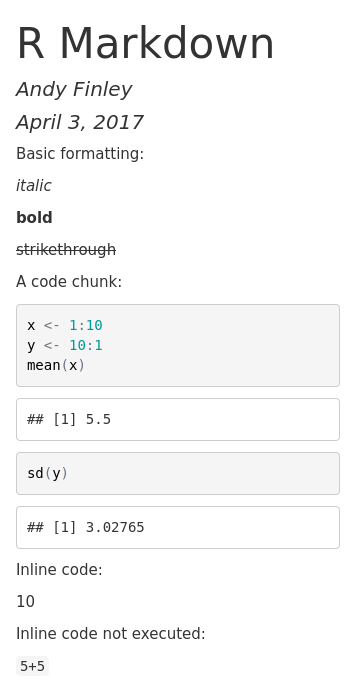
\includegraphics[width=4.9in]{../figures/Small-2} \caption{Output from the above R Markdown code}\label{fig:rmdOut}
\end{figure}

At the top of the input R Markdown file are some lines with
\texttt{-\/-\/-} at the top and bottom. These lines are not needed, but
give a convenient way to specify the title, author, and date of the
article that are then typeset prominently at the top of the output
document. For now, don't be concerned with the lines following
\texttt{output:}. These can be omitted (or included as shown).

Next are a few lines showing some of the ways that font effects such as
italics, boldface, and strikethrough can be achieved. For example, an
asterisk before and after text sets the text in \emph{italics}, and two
asterisks before and after text sets the text in \emph{boldface}.

More important for our purposes is the ability to include R code in the
R Markdown file, which will be executed with the output appearing in the
output document. Bits of R code included this way are called \emph{code
chunks}. The beginning of a code chunk is indicated with three backticks
and an ``r'' in curly braces:
\texttt{\textasciigrave{}\textasciigrave{}\textasciigrave{}\{r\}}. The
end of a code chunk is indicated with three backticks:
\texttt{\textasciigrave{}\textasciigrave{}\textasciigrave{}}. For
example, the R Markdown file described above has one code chunk:

\begin{verbatim}
```{r}
x <- 1:10
y <- 10:1
mean(x)
sd(y)
```
\end{verbatim}

In this code chunk two vectors \texttt{x} and \texttt{y} are created,
and the mean of \texttt{x} and the standard deviation of \texttt{y} are
computed. In the output in Figure \ref{fig:rmdOut} the R code is
reproduced, and the output of the two lines of code asking for the mean
and standard deviation is shown.

\subsection{Creating and Processing R Markdown
Documents}\label{creating-and-processing-r-markdown-documents}

RStudio has features which facilitate creating and processing R Markdown
documents. Choose
\texttt{File\ \textgreater{}\ New\ File\ \textgreater{}\ R\ \ Markdown...}.
In the ensuing dialog box make sure that \texttt{Document} is
highlighted on the left, enter the title and author (if desired), and
choose the Default Output Format (HTML is good to begin). Then click OK.
A document will appear in the upper left of the RStudio window. It is an
R Markdown document, and the title and author you chose will show up,
delimited by \texttt{-\/-\/-} at the top of the document. A generic body
of the document will also be included.

For now just keep this generic document as is. To process it to create
the HTML output, click the \texttt{Knit\ HTML} button at the top of the
R Markdown window. You'll be prompted to choose a filename for the R
Markdown file. Use \texttt{.Rmd} as the extension for this file. Once
you've saved the file, RStudio will process the file, create the HTML
output, and open this output in a new window. The HTML output file will
also be saved to your working directory. This file can be shared with
others, who can open it using a web browser such as Chrome or Firefox.

There are many options which allow customization of R Markdown
documents. Some of these affect formatting of text in the document,
while others affect how R code is evaluated and displayed. The RStudio
web site contains a useful summary of many R Markdown options at
www.rstudio.com/wp-content/uploads/2015/03/rmarkdown-reference.pdf. A
different, but mind-numbingly busy, cheatsheet is at
www.rstudio.com/wp-content/uploads/2016/03/rmarkdown-cheatsheet-2.0.pdf.
Some of the more commonly used R Markdown options are described next.

\subsubsection{Text: Lists and Headers}\label{text-lists-and-headers}

Unordered (sometimes called bulleted) lists and ordered lists are easy
in R Markdown. Below we illustrate the creation of unordered and ordered
lists.

\begin{itemize}
\tightlist
\item
  For an unordered list, either an asterisk, a plus sign, or a minus
  sign may precede list items. Use a space after these symbols before
  including the list text. To have second-level items (sub-lists) indent
  four spaces before indicating the list item. This can also be done for
  third-level items.
\item
  For an ordered list use a numeral followed by a period and a space (1.
  or 2. or 3. or \ldots{}) to indicate a numbered list, and use a letter
  followed by a period and a space (a. or b. or c. or \ldots{}) to
  indicate a lettered list. The same four space convention is used to
  designate sub lists.
\item
  For an ordered list, the first list item will be labeled with the
  number or letter that you specify, but subsequent list items will be
  numbered sequentially. This will become clear through the following
  example. Consider the R Markdown input below and the subsequent output
  in Figure \ref{fig:listOut}:
\end{itemize}

\begin{verbatim}
An unordered list:

* List item 1
* List item 2
    + Second level list item 1
    + Second level list item 2
        + Third level list item
* List item 3

An ordered list:

1. List item 1
2. List item 2
    c. Sub list item 1
    q. Sub list item 2
17. List item 3
\end{verbatim}

\begin{Shaded}
\begin{Highlighting}[]
\OperatorTok{>}\StringTok{ }\KeywordTok{include_graphics}\NormalTok{(}\StringTok{"../figures/ListExamples.pdf"}\NormalTok{)}
\end{Highlighting}
\end{Shaded}

\begin{figure}
\centering
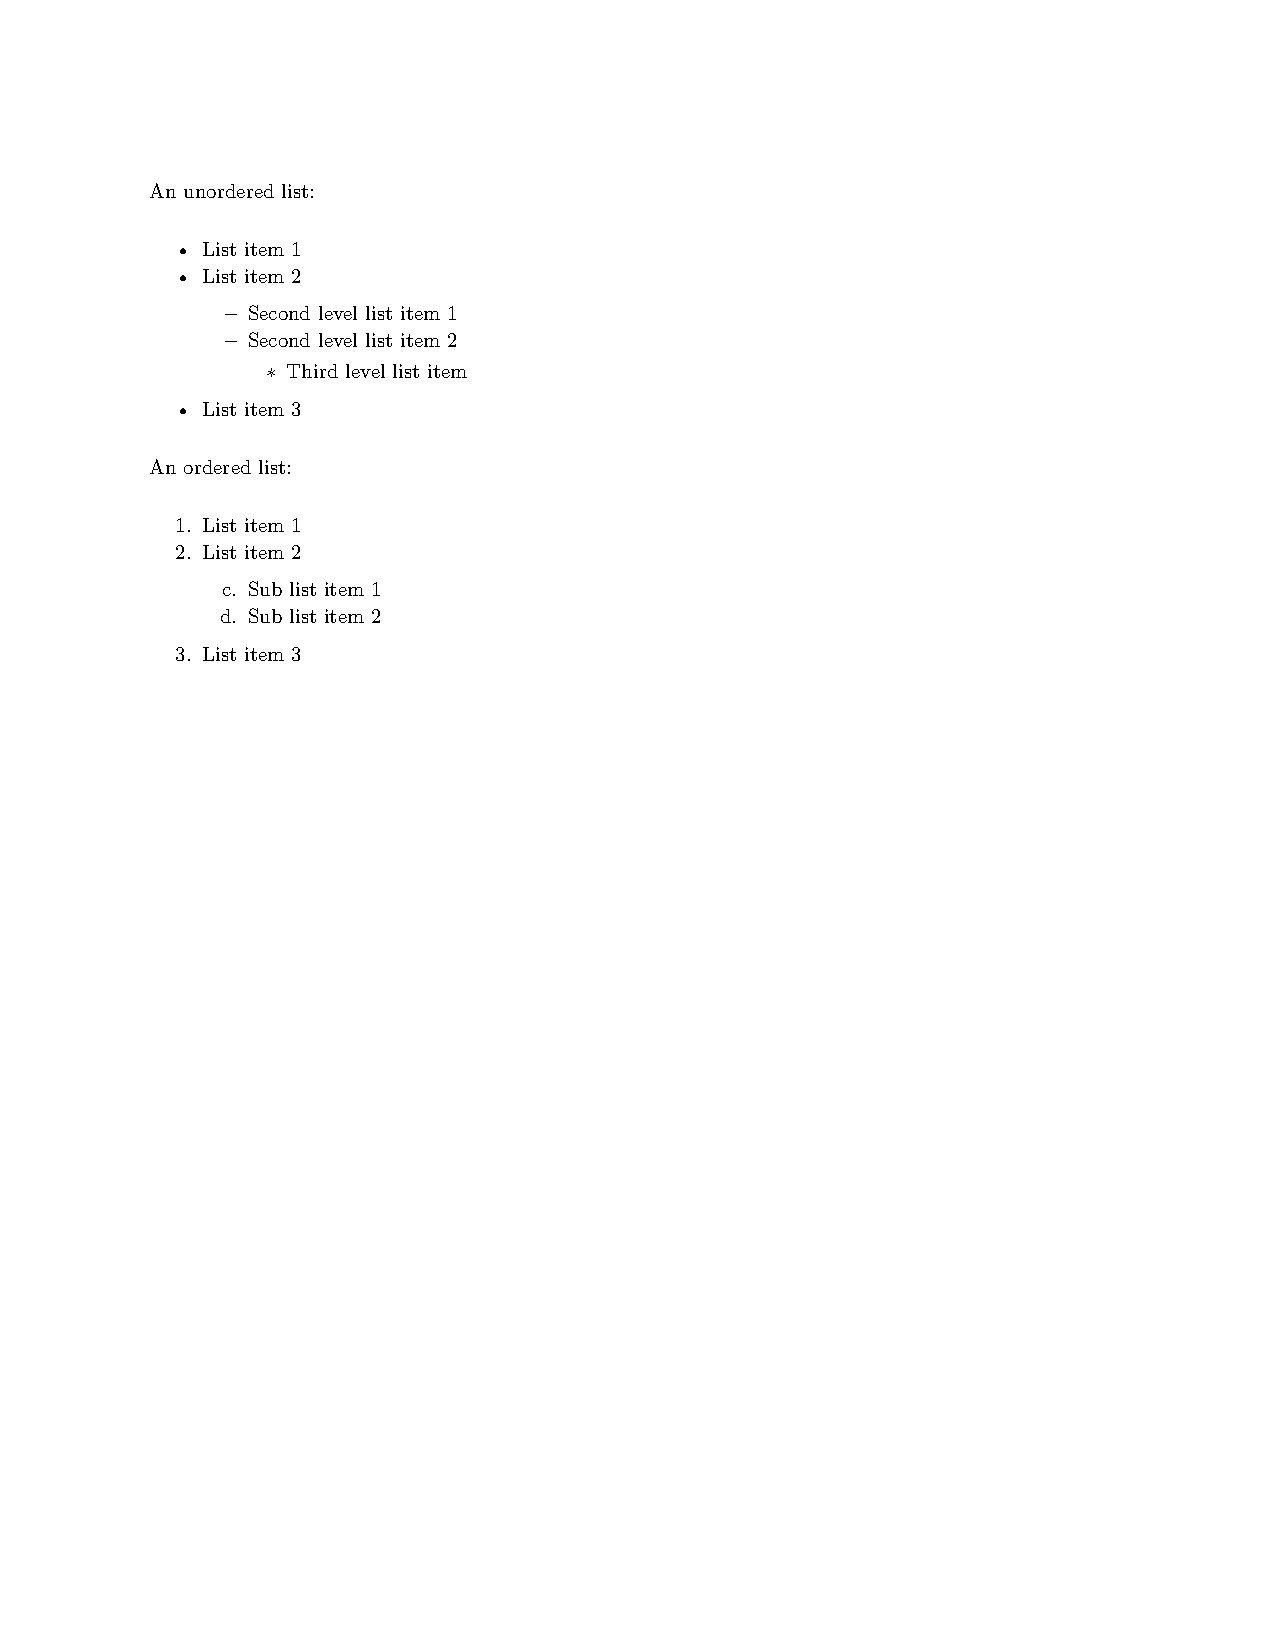
\includegraphics{../figures/ListExamples.pdf}
\caption{\label{fig:listOut}R Markdown List Output}
\end{figure}

In those examples notice that for the ordered list, although the
first-level numbers given in the R Markdown code are 1, 2, and 17, the
numbers printed in the output are 1, 2, and 3. Similarly the letters
given in the R Markdown code are c and q, but the output file prints c
and d.

R Markdown does not give substantial control over font size. Different
``header'' levels, which provide different font sizes, are available.
Put one or more hash marks (\#) in front of text to specify different
header levels. Other font choices such as subscripts and superscripts
are possible, by surrounding the text either by tildes or carets,
respectively. More sophisticated mathematical displays are also
possible, and are surrounded by dollar signs. The actual mathematical
expressions are specified using a language called LaTeX. See the
examples below for further information for working with headers in R
Markdown and LaTeX commands.

\begin{verbatim}
# A first *level* ~~header~~

## A second level header

### A third level header

Text subscripts and superscripts:

x~2~ + y~2~

10^3^ = 1000

Mathematics examples:

$x_a$

$x^a$

$\int_0^1 x^2 dx$

$\frac{x}{y}$

$\sqrt{x}$

$\sqrt[n]{x}$

$\sum_{k=1}^n$

$\prod_{k=1}^n$
\end{verbatim}

\begin{figure}
\centering
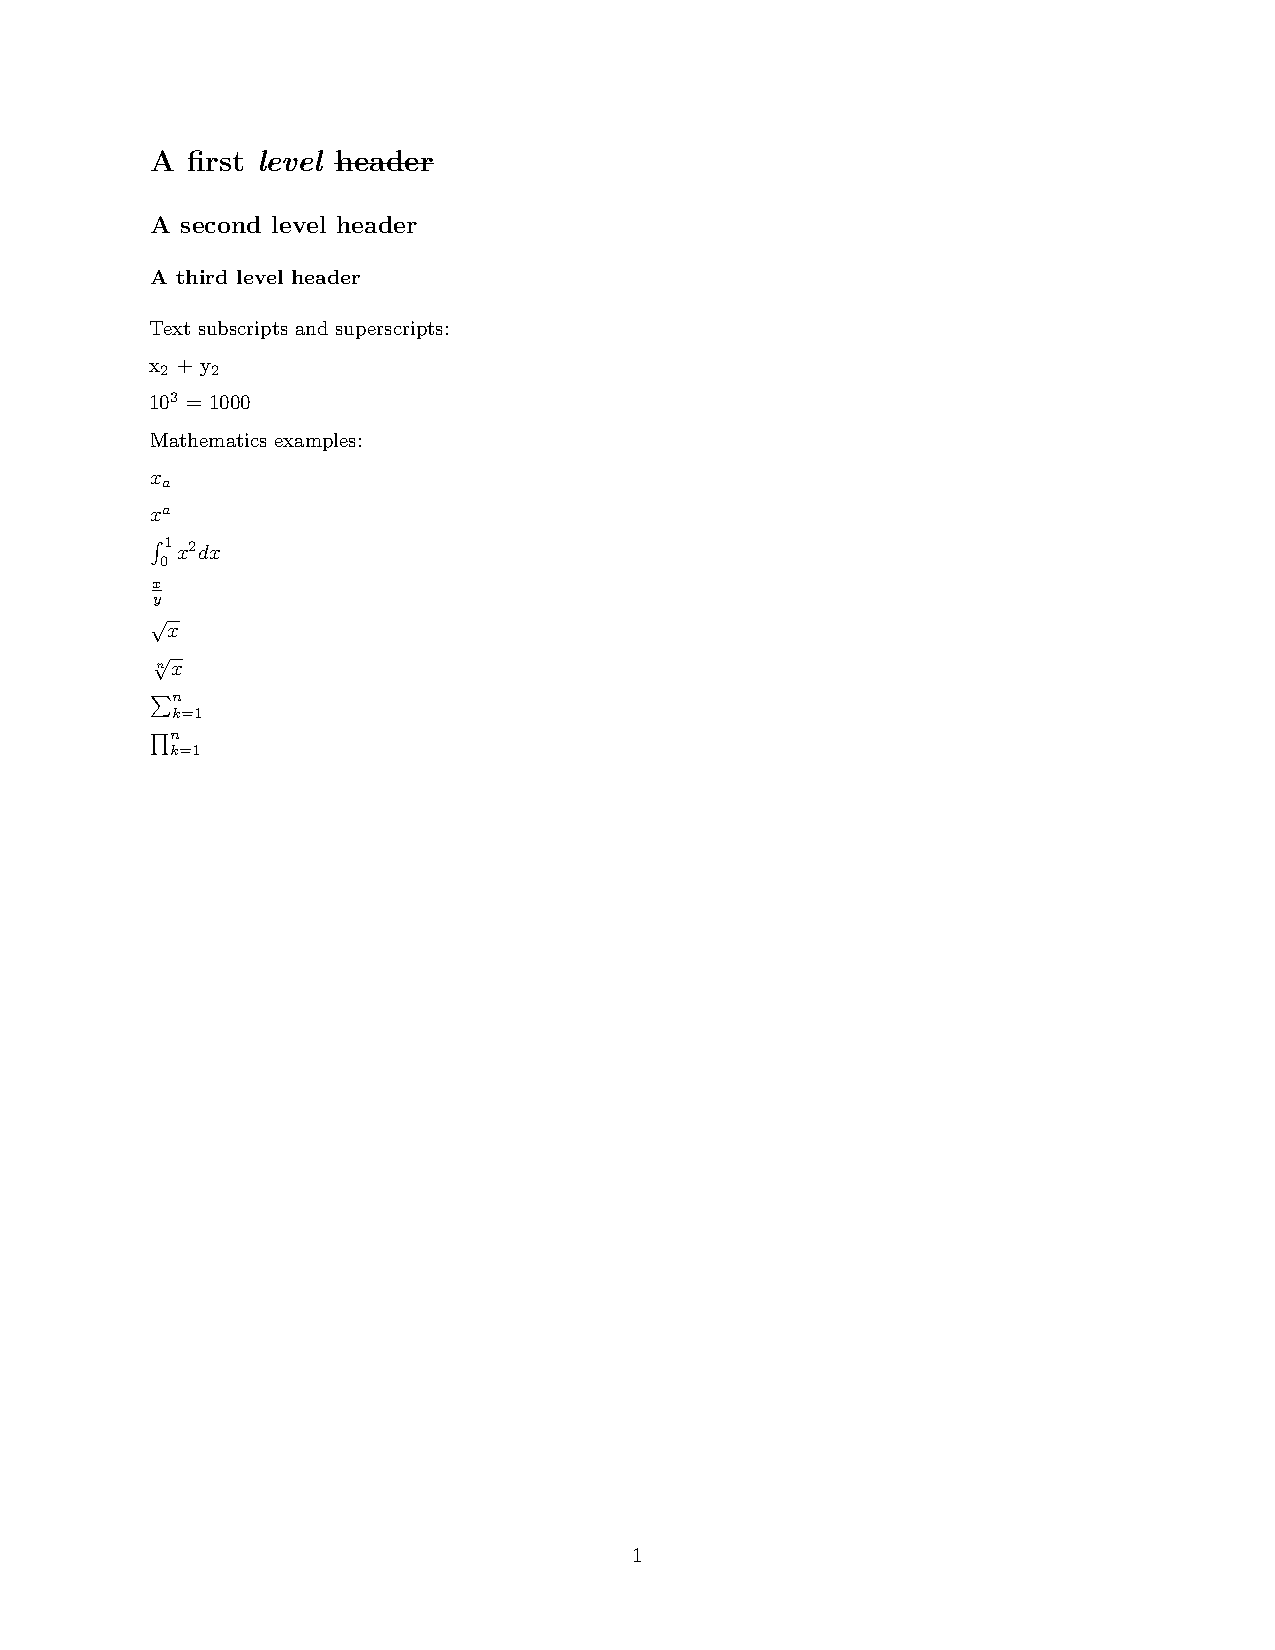
\includegraphics{../figures/headers.pdf}
\caption{\label{fig:headerOut}More R Markdown Output}
\end{figure}

\begin{figure}
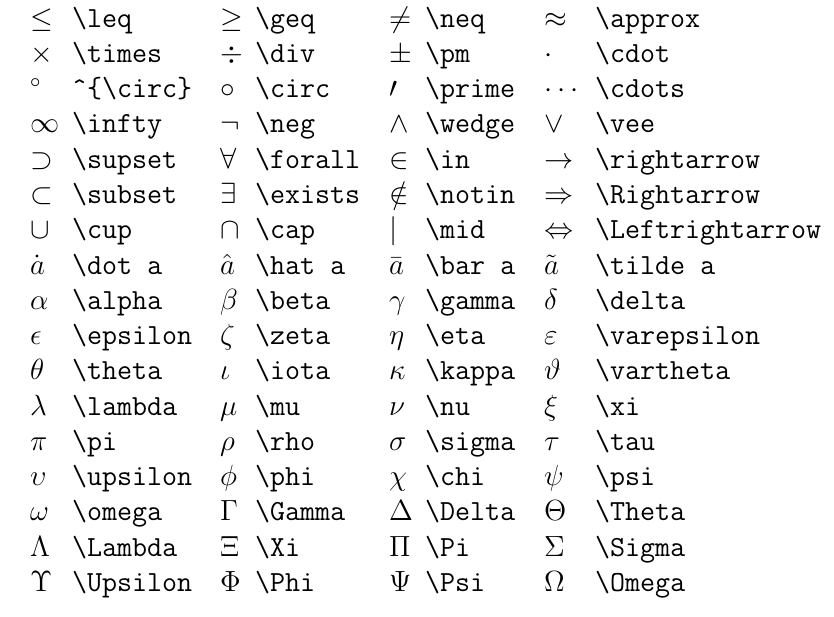
\includegraphics[width=11.58in]{../figures/latexExpressions} \caption{Other useful LaTeX expressions and symboles available for use in R Markdown}\label{fig:latexOut}
\end{figure}

\subsubsection{Code Chunks}\label{code-chunks}

R Markdown provides a large number of options to vary the behavior of
code chunks. In some contexts it is useful to display the output but not
the R code leading to the output. In some contexts it is useful to
display the R prompt and in others it is not. Perhaps it is useful to
configure the size of figures created by graphics. And so on. These code
chunk options and many more are described in
www.rstudio.com/wp-content/uploads/2015/03/rmarkdown-reference.pdf.

Code chunk options are specified in the curly braces near the beginning
of a code chunk. For example the option \texttt{echo=FALSE} would be
specified via
\texttt{\textasciigrave{}\textasciigrave{}\textasciigrave{}\{r,\ echo=FALSE\}}.
Below are descriptions of a few of the more commonly used options. The
use of these options is illustrated in
Figures\textasciitilde{}\ref{FIG:CODE_CHUNK_OPTIONS1}
and\textasciitilde{}\ref{FIG:CODE_CHUNK_OPTIONS2}.

\begin{enumerate}
\def\labelenumi{\arabic{enumi}.}
\item
  \texttt{echo=FALSE} specifies that the R code should not be printed
  (but any output of the R code should be printed) in the resulting
  document.
\item
  \texttt{include=FALSE} specifies that neither the R code nor the
  output should be printed. However, the objects created by the code
  chunk will be available for use in later code chunks.
\item
  \texttt{eval=FALSE} specifies that the R code should not be evaluated.
  The code will be printed unless, for example, \texttt{echo=FALSE} is
  also given as an option.
\item
  \texttt{error=FALSE} and \texttt{warning=FALSE} specify that,
  respectively, error messages and warning messages generated by the R
  code should not be printed.
\item
  The \texttt{comment} option allows a specified character string to be
  prepended to each line of results. By default this is set to
  \texttt{comment\ =\ \textquotesingle{}\#\#\textquotesingle{}} which
  explains the two hash marks preceding results in Figure
  \ref{fig:rmdOut} for example. Setting \texttt{comment\ =\ NA} presents
  output without any character string prepended. That is done in most
  code chunks in this book.
\item
  \texttt{prompt=TRUE} specifies that R prompt \texttt{\textgreater{}}
  will be prepended to each line of R code shown in the document.
  \texttt{prompt\ =\ FALSE} specifies that command prompts should not be
  included.
\item
  \texttt{fig.height} and \texttt{fig.width} specify the height and
  width of figures generated by R code. These are specified in inches,
  so for example \texttt{fig.height=4} specifies a four inch high
  figure.
\end{enumerate}

The below R Markdown input and \ref{fig:codeOptions} (printed output)
give examples of the use of code chunk options.

```

No options:

\begin{verbatim}
x <- 1:10
x
\end{verbatim}

echo=FALSE: \texttt{\{r,\ echo\ =\ FALSE\}\ x\ \textless{}-\ 1:10\ x}

comment=NA: \texttt{\{r,\ comment\ =\ NA\}\ x\ \textless{}-\ 1:10\ x}
comment=`\#', prompt=TRUE:
\texttt{\{r,\ comment\ =\ \textquotesingle{}\#\textquotesingle{},\ prompt\ =\ TRUE\}\ x\ \textless{}-\ 1:10\ x}

echo=FALSE, fig.height=4, fig.width=4:

\texttt{\{r,\ echo\ =\ FALSE,\ fig.height\ =\ 4,\ fig.width\ =\ 4\}\ y\ \textless{}-\ 10:1\ plot(x,y)}

```

\begin{figure}
\centering
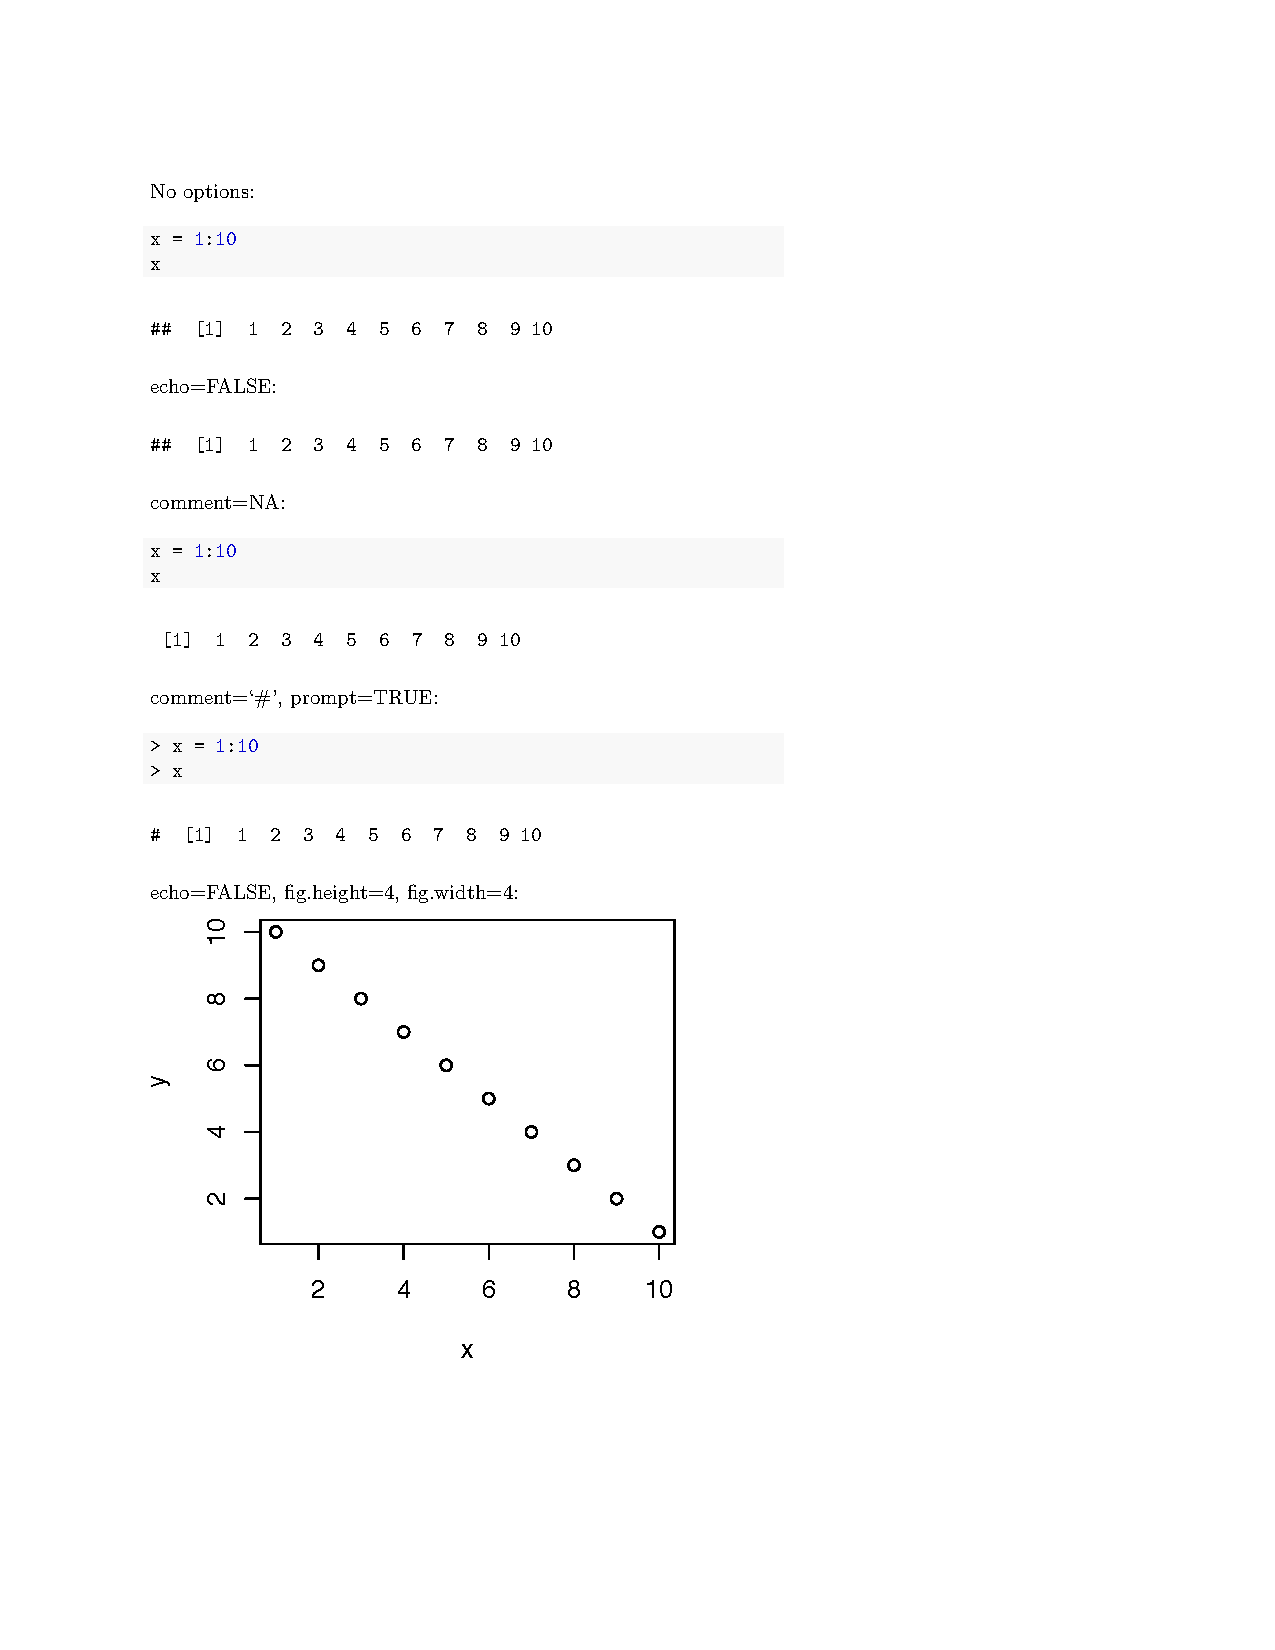
\includegraphics{../figures/CodeChunkOptions.pdf}
\caption{\label{fig:codeOptions}Output of Example R Code Chunk Options}
\end{figure}

\subsection{Output Formats other than
HTML}\label{output-formats-other-than-html}

It is possible to use R Markdown to produce documents in formats other
than HTML, including Word and PDF documents, among others. Next to the
\texttt{Knit\ HTML} button is a down arrow. Click on this and choose
\texttt{Knit\ Word} to produce a Microsoft word output document.
Although there is also a \texttt{Knit\ PDF} button, PDF output requires
additional software called TeX in addition to RStudio.\footnote{It isn't
  particularly hard to install TeX software. For a Microsoft Windows
  system, MiKTeX is convenient, and is available from miktex.org. For a
  Mac system, MacTeX is available from www.tug.org/mactex/.}

\subsection{\texorpdfstring{LaTeX, \texttt{knitr}, and
\texttt{bookdown}}{LaTeX, knitr, and bookdown}}\label{latex-knitr-and-bookdown}

While basic R Markdown provides substantial flexibility and power, it
lacks features such as cross-referencing, fine control over fonts, etc.
If this is desired, a variant of R Markdown called \texttt{knitr}, which
has very similar syntax to R Markdown for code chunks, can be used in
conjunction with the typesetting system LaTeX to produce documents.
Another option is to use the R package \texttt{bookdown} which uses R
Markdown syntax and some additional features to allow for writing more
technical documents. In fact this book was initially created using
\texttt{knitr} and LaTeX, but the simplicity of markdown syntax and the
additional intricacies provided by the \texttt{bookdown} package
convinced us to write the book in R Markdown using \texttt{bookdown}.
For simpler tasks, basic R Markdown is plenty sufficient, and very easy
to use.

\section{Practice Exercises}\label{practice-exercises}

\section{Homework}\label{homework}

\textbf{Exercise 1} Learning objectives: practice setting up a working
directory and read in data; explore the workspace within RStudio and
associated commands; produce basic descriptive statistics and graphics.

\textbf{Exercise 2} Learning objectives: practice working within
RStudio; create a R Markdown document and resulting html document in
RStudio; calculate descriptive statistics and produce graphics.

\chapter{Data Structures}\label{structures}

A data structure is a format for organizing and storing data. The
structure is designed so that data can be accessed and worked with in
specific ways. Statistical software and programming languages have
methods (or functions) designed to operate on different kinds of data
structures.

This chapter's focus is on data structures. To help initial
understanding, the data in this chapter will be relatively modest in
size and complexity. The ideas and methods, however, generalize to
larger and more complex data sets.

The base data structures in R are vectors, matrices, arrays, data
frames, and lists. The first three, vectors, matrices, and arrays,
require all elements to be of the same type or homogeneous, e.g., all
numeric or all character. Data frames and lists allow elements to be of
different types or heterogeneous, e.g., some elements of a data frame
may be numeric while other elements may be character. These base
structures can also be organized by their dimensionality, i.e.,
1-dimensional, 2-dimensional, or N-dimensional, as shown in Table
\ref{tab:dataStructures}.

\begin{table}

\caption{\label{tab:dataStructures}Dimension and type content of base data structures
  in R}
\centering
\begin{tabular}[t]{lll}
\toprule
Dimension & Homogeneous & Heterogeneous\\
\midrule
1 & Atomic vector & List\\
2 & Matrix & Data frame\\
N & Array & \\
\bottomrule
\end{tabular}
\end{table}

R has no scalar types, i.e., 0-dimensional. Individual numbers or
strings are actually vectors of length one.

An efficient way to understand what comprises a given object is to use
the \texttt{str()} function. \texttt{str()} is short for structure and
prints a compact, human-readable description of any R data structure.
For example, in the code below, we prove to ourselves that what we might
think of as a scalar value is actually a vector of length one.

\begin{Shaded}
\begin{Highlighting}[]
\OperatorTok{>}\StringTok{ }\NormalTok{a <-}\StringTok{ }\DecValTok{1}
\OperatorTok{>}\StringTok{ }\KeywordTok{str}\NormalTok{(a)}
\end{Highlighting}
\end{Shaded}

\begin{verbatim}
 num 1
\end{verbatim}

\begin{Shaded}
\begin{Highlighting}[]
\OperatorTok{>}\StringTok{ }\KeywordTok{is.vector}\NormalTok{(a)}
\end{Highlighting}
\end{Shaded}

\begin{verbatim}
[1] TRUE
\end{verbatim}

\begin{Shaded}
\begin{Highlighting}[]
\OperatorTok{>}\StringTok{ }\KeywordTok{length}\NormalTok{(a)}
\end{Highlighting}
\end{Shaded}

\begin{verbatim}
[1] 1
\end{verbatim}

Here we assigned \texttt{a} the scalar value one. The \texttt{str(a)}
prints \texttt{num\ 1}, which says \texttt{a} is numeric of length one.
Then just to be sure we used the function \texttt{is.vector()} to test
if \texttt{a} is in fact a vector. Then, just for fun, we asked the
length of \texttt{a}, which again returns one. There are a set of
similar logical tests for the other base data structures, e.g.,
\texttt{is.matrix()}, \texttt{is.array()}, \texttt{is.data.frame()}, and
\texttt{is.list()}. These will all come in handy as we encounter
different R objects.

\section{Vectors}\label{vector}

Think of a vector\footnote{Technically the objects described in this
  section are ``atomic'' vectors (all elements of the same type), since
  lists, to be described below, also are actually vectors. This will not
  be an important issue, and the shorter term vector will be used for
  atomic vectors below.} as a structure to represent one variable in a
data set. For example a vector might hold the weights, in pounds, of 7
people in a data set. Or another vector might hold the genders of those
7 people. The \texttt{c()} function in R is useful for creating (small)
vectors and for modifying existing vectors. Think of \texttt{c} as
standing for ``combine''.

\begin{Shaded}
\begin{Highlighting}[]
\OperatorTok{>}\StringTok{ }\NormalTok{weight <-}\StringTok{ }\KeywordTok{c}\NormalTok{(}\DecValTok{123}\NormalTok{, }\DecValTok{157}\NormalTok{, }\DecValTok{205}\NormalTok{, }\DecValTok{199}\NormalTok{, }\DecValTok{223}\NormalTok{, }\DecValTok{140}\NormalTok{, }\DecValTok{105}\NormalTok{)}
\OperatorTok{>}\StringTok{ }\NormalTok{weight}
\end{Highlighting}
\end{Shaded}

\begin{verbatim}
[1] 123 157 205 199 223 140 105
\end{verbatim}

\begin{Shaded}
\begin{Highlighting}[]
\OperatorTok{>}\StringTok{ }\NormalTok{gender <-}\StringTok{ }\KeywordTok{c}\NormalTok{(}\StringTok{"female"}\NormalTok{, }\StringTok{"female"}\NormalTok{, }\StringTok{"male"}\NormalTok{, }\StringTok{"female"}\NormalTok{, }\StringTok{"male"}\NormalTok{, }
\OperatorTok{+}\StringTok{             "male"}\NormalTok{, }\StringTok{"female"}\NormalTok{)}
\OperatorTok{>}\StringTok{ }\NormalTok{gender}
\end{Highlighting}
\end{Shaded}

\begin{verbatim}
[1] "female" "female" "male"   "female" "male"  
[6] "male"   "female"
\end{verbatim}

Notice that elements of a vector are separated by commas when using the
\texttt{c()} function to create a vector. Also notice that character
values are placed inside quotation marks.

The \texttt{c()} function also can be used to add to an existing vector.
For example, if an eighth male person was included in the data set, and
his weight was 194 pounds, the existing vectors could be modified as
follows.

\begin{Shaded}
\begin{Highlighting}[]
\OperatorTok{>}\StringTok{ }\NormalTok{weight <-}\StringTok{ }\KeywordTok{c}\NormalTok{(weight, }\DecValTok{194}\NormalTok{)}
\OperatorTok{>}\StringTok{ }\NormalTok{gender <-}\StringTok{ }\KeywordTok{c}\NormalTok{(gender, }\StringTok{"male"}\NormalTok{)}
\OperatorTok{>}\StringTok{ }\NormalTok{weight}
\end{Highlighting}
\end{Shaded}

\begin{verbatim}
[1] 123 157 205 199 223 140 105 194
\end{verbatim}

\begin{Shaded}
\begin{Highlighting}[]
\OperatorTok{>}\StringTok{ }\NormalTok{gender}
\end{Highlighting}
\end{Shaded}

\begin{verbatim}
[1] "female" "female" "male"   "female" "male"  
[6] "male"   "female" "male"  
\end{verbatim}

\subsection{Types, Conversion,
Coercion}\label{types-conversion-coercion}

Clearly it is important to distinguish between different types of
vectors. For example, it makes sense to ask R to calculate the mean of
the weights stored in \texttt{weight}, but does not make sense to ask R
to compute the mean of the genders stored in \texttt{gender}. Vectors in
R may have one of six different ``types'': character, double, integer,
logical, complex, and raw. Only the first four of these will be of
interest below, and the distinction between double and integer will not
be of great import. To illustrate logical vectors, imagine that each of
the eight people in the data set was asked whether he or she was taking
blood pressure medication, and the responses were coded as \texttt{TRUE}
if the person answered yes, and \texttt{FALSE} if the person answered
no.

\begin{Shaded}
\begin{Highlighting}[]
\OperatorTok{>}\StringTok{ }\KeywordTok{typeof}\NormalTok{(weight)}
\end{Highlighting}
\end{Shaded}

\begin{verbatim}
[1] "double"
\end{verbatim}

\begin{Shaded}
\begin{Highlighting}[]
\OperatorTok{>}\StringTok{ }\KeywordTok{typeof}\NormalTok{(gender)}
\end{Highlighting}
\end{Shaded}

\begin{verbatim}
[1] "character"
\end{verbatim}

\begin{Shaded}
\begin{Highlighting}[]
\OperatorTok{>}\StringTok{ }\NormalTok{bp <-}\StringTok{ }\KeywordTok{c}\NormalTok{(}\OtherTok{FALSE}\NormalTok{, }\OtherTok{TRUE}\NormalTok{, }\OtherTok{FALSE}\NormalTok{, }\OtherTok{FALSE}\NormalTok{, }\OtherTok{TRUE}\NormalTok{, }\OtherTok{FALSE}\NormalTok{, }\OtherTok{TRUE}\NormalTok{, }\OtherTok{FALSE}\NormalTok{)}
\OperatorTok{>}\StringTok{ }\NormalTok{bp}
\end{Highlighting}
\end{Shaded}

\begin{verbatim}
[1] FALSE  TRUE FALSE FALSE  TRUE FALSE  TRUE FALSE
\end{verbatim}

\begin{Shaded}
\begin{Highlighting}[]
\OperatorTok{>}\StringTok{ }\KeywordTok{typeof}\NormalTok{(bp)}
\end{Highlighting}
\end{Shaded}

\begin{verbatim}
[1] "logical"
\end{verbatim}

It may be surprising to see that the variable \texttt{weight} is of
\texttt{double} type, even though its values all are integers. By
default R creates a double type vector when numeric values are given via
the \texttt{+c()} function.

When it makes sense, it is possible to convert vectors to a different
type. Consider the following examples.

\begin{Shaded}
\begin{Highlighting}[]
\OperatorTok{>}\StringTok{ }\NormalTok{weight.int <-}\StringTok{ }\KeywordTok{as.integer}\NormalTok{(weight)}
\OperatorTok{>}\StringTok{ }\NormalTok{weight.int}
\end{Highlighting}
\end{Shaded}

\begin{verbatim}
[1] 123 157 205 199 223 140 105 194
\end{verbatim}

\begin{Shaded}
\begin{Highlighting}[]
\OperatorTok{>}\StringTok{ }\KeywordTok{typeof}\NormalTok{(weight.int)}
\end{Highlighting}
\end{Shaded}

\begin{verbatim}
[1] "integer"
\end{verbatim}

\begin{Shaded}
\begin{Highlighting}[]
\OperatorTok{>}\StringTok{ }\NormalTok{weight.char <-}\StringTok{ }\KeywordTok{as.character}\NormalTok{(weight)}
\OperatorTok{>}\StringTok{ }\NormalTok{weight.char}
\end{Highlighting}
\end{Shaded}

\begin{verbatim}
[1] "123" "157" "205" "199" "223" "140" "105" "194"
\end{verbatim}

\begin{Shaded}
\begin{Highlighting}[]
\OperatorTok{>}\StringTok{ }\NormalTok{bp.double <-}\StringTok{ }\KeywordTok{as.double}\NormalTok{(bp)}
\OperatorTok{>}\StringTok{ }\NormalTok{bp.double}
\end{Highlighting}
\end{Shaded}

\begin{verbatim}
[1] 0 1 0 0 1 0 1 0
\end{verbatim}

\begin{Shaded}
\begin{Highlighting}[]
\OperatorTok{>}\StringTok{ }\NormalTok{gender.oops <-}\StringTok{ }\KeywordTok{as.double}\NormalTok{(gender)}
\end{Highlighting}
\end{Shaded}

\begin{verbatim}
Warning: NAs introduced by coercion
\end{verbatim}

\begin{Shaded}
\begin{Highlighting}[]
\OperatorTok{>}\StringTok{ }\NormalTok{gender.oops}
\end{Highlighting}
\end{Shaded}

\begin{verbatim}
[1] NA NA NA NA NA NA NA NA
\end{verbatim}

\begin{Shaded}
\begin{Highlighting}[]
\OperatorTok{>}\StringTok{ }\KeywordTok{sum}\NormalTok{(bp)}
\end{Highlighting}
\end{Shaded}

\begin{verbatim}
[1] 3
\end{verbatim}

The integer version of \texttt{weight} doesn't look any different, but
it is stored differently, which can be important both for computational
efficiency and for interfacing with other languages such as
\texttt{C++}. As noted above, however, we will not worry about the
distinction between integer and double types. Converting \texttt{weight}
to character goes as expected: The character representations of the
numbers replace the numbers themselves. Converting the logical vector
\texttt{bp} to double is pretty straightforward too: \texttt{FALSE} is
converted to zero, and \texttt{TRUE} is converted to one. Now think
about converting the character vector \texttt{gender} to a numeric
double vector. It's not at all clear how to represent ``female'' and
``male'' as numbers. In fact in this case what R does is to create a
character vector, but with each element set to \texttt{NA}, which is the
representation of missing data.\footnote{Missing data will be discussed
  in more detail later in the chapter.} Finally consider the code
\texttt{sum(bp)}. Now \texttt{bp} is a logical vector, but when R sees
that we are asking to sum this logical vector, it automatically converts
it to a numerical vector and then adds the zeros and ones representing
\texttt{FALSE} and \texttt{TRUE}.

R also has functions to test whether a vector is of a particular type.

\begin{Shaded}
\begin{Highlighting}[]
\OperatorTok{>}\StringTok{ }\KeywordTok{is.double}\NormalTok{(weight)}
\end{Highlighting}
\end{Shaded}

\begin{verbatim}
[1] TRUE
\end{verbatim}

\begin{Shaded}
\begin{Highlighting}[]
\OperatorTok{>}\StringTok{ }\KeywordTok{is.character}\NormalTok{(weight)}
\end{Highlighting}
\end{Shaded}

\begin{verbatim}
[1] FALSE
\end{verbatim}

\begin{Shaded}
\begin{Highlighting}[]
\OperatorTok{>}\StringTok{ }\KeywordTok{is.integer}\NormalTok{(weight.int)}
\end{Highlighting}
\end{Shaded}

\begin{verbatim}
[1] TRUE
\end{verbatim}

\begin{Shaded}
\begin{Highlighting}[]
\OperatorTok{>}\StringTok{ }\KeywordTok{is.logical}\NormalTok{(bp)}
\end{Highlighting}
\end{Shaded}

\begin{verbatim}
[1] TRUE
\end{verbatim}

\subsubsection{Coercion}\label{coercion}

Consider the following examples.

\begin{Shaded}
\begin{Highlighting}[]
\OperatorTok{>}\StringTok{ }\NormalTok{xx <-}\StringTok{ }\KeywordTok{c}\NormalTok{(}\DecValTok{1}\NormalTok{, }\DecValTok{2}\NormalTok{, }\DecValTok{3}\NormalTok{, }\OtherTok{TRUE}\NormalTok{)}
\OperatorTok{>}\StringTok{ }\NormalTok{xx}
\end{Highlighting}
\end{Shaded}

\begin{verbatim}
[1] 1 2 3 1
\end{verbatim}

\begin{Shaded}
\begin{Highlighting}[]
\OperatorTok{>}\StringTok{ }\NormalTok{yy <-}\StringTok{ }\KeywordTok{c}\NormalTok{(}\DecValTok{1}\NormalTok{, }\DecValTok{2}\NormalTok{, }\DecValTok{3}\NormalTok{, }\StringTok{"dog"}\NormalTok{)}
\OperatorTok{>}\StringTok{ }\NormalTok{yy}
\end{Highlighting}
\end{Shaded}

\begin{verbatim}
[1] "1"   "2"   "3"   "dog"
\end{verbatim}

\begin{Shaded}
\begin{Highlighting}[]
\OperatorTok{>}\StringTok{ }\NormalTok{zz <-}\StringTok{ }\KeywordTok{c}\NormalTok{(}\OtherTok{TRUE}\NormalTok{, }\OtherTok{FALSE}\NormalTok{, }\StringTok{"cat"}\NormalTok{)}
\OperatorTok{>}\StringTok{ }\NormalTok{zz}
\end{Highlighting}
\end{Shaded}

\begin{verbatim}
[1] "TRUE"  "FALSE" "cat"  
\end{verbatim}

\begin{Shaded}
\begin{Highlighting}[]
\OperatorTok{>}\StringTok{ }\NormalTok{weight }\OperatorTok{+}\StringTok{ }\NormalTok{bp}
\end{Highlighting}
\end{Shaded}

\begin{verbatim}
[1] 123 158 205 199 224 140 106 194
\end{verbatim}

Vectors in R can only contain elements of one type. If more than one
type is included in a \texttt{c()} function, R silently \emph{coerces}
the vector to be of one type. The examples illustrate the hierarchy---if
any element is a character, then the whole vector is character. If some
elements are numeric (either integer or double) and other elements are
logical, the whole vector is numeric. Note what happened when R was
asked to add the numeric vector \texttt{weight} to the logical vector
\texttt{bp}. The logical vector was silently coerced to be numeric, so
that FALSE became zero and TRUE became one, and then the two numeric
vectors were added.

\subsection{Accessing Specific Elements of
Vectors}\label{accessing-specific-elements-of-vectors}

To access and possibly change specific elements of vectors, refer to the
position of the element in square brackets. For example,
\texttt{weight{[}4{]}} refers to the fourth element of the vector
\texttt{weight}. Note that R starts the numbering of elements at 1,
i.e., the first element of a vector \texttt{x} is \texttt{x{[}1{]}}.

\begin{Shaded}
\begin{Highlighting}[]
\OperatorTok{>}\StringTok{ }\NormalTok{weight}
\end{Highlighting}
\end{Shaded}

\begin{verbatim}
[1] 123 157 205 199 223 140 105 194
\end{verbatim}

\begin{Shaded}
\begin{Highlighting}[]
\OperatorTok{>}\StringTok{ }\NormalTok{weight[}\DecValTok{5}\NormalTok{]}
\end{Highlighting}
\end{Shaded}

\begin{verbatim}
[1] 223
\end{verbatim}

\begin{Shaded}
\begin{Highlighting}[]
\OperatorTok{>}\StringTok{ }\NormalTok{weight[}\DecValTok{1}\OperatorTok{:}\DecValTok{3}\NormalTok{]}
\end{Highlighting}
\end{Shaded}

\begin{verbatim}
[1] 123 157 205
\end{verbatim}

\begin{Shaded}
\begin{Highlighting}[]
\OperatorTok{>}\StringTok{ }\KeywordTok{length}\NormalTok{(weight)}
\end{Highlighting}
\end{Shaded}

\begin{verbatim}
[1] 8
\end{verbatim}

\begin{Shaded}
\begin{Highlighting}[]
\OperatorTok{>}\StringTok{ }\NormalTok{weight[}\KeywordTok{length}\NormalTok{(weight)]}
\end{Highlighting}
\end{Shaded}

\begin{verbatim}
[1] 194
\end{verbatim}

\begin{Shaded}
\begin{Highlighting}[]
\OperatorTok{>}\StringTok{ }\NormalTok{weight[]}
\end{Highlighting}
\end{Shaded}

\begin{verbatim}
[1] 123 157 205 199 223 140 105 194
\end{verbatim}

\begin{Shaded}
\begin{Highlighting}[]
\OperatorTok{>}\StringTok{ }\NormalTok{weight[}\DecValTok{3}\NormalTok{] <-}\StringTok{ }\DecValTok{202}
\OperatorTok{>}\StringTok{ }\NormalTok{weight}
\end{Highlighting}
\end{Shaded}

\begin{verbatim}
[1] 123 157 202 199 223 140 105 194
\end{verbatim}

Note that including nothing in the square brackets results in the whole
vector being returned.

Negative numbers in the square brackets tell R to omit the corresponding
value. And a zero as a subscript returns nothing (more precisely, it
returns a length zero vector of the appropriate type).

\begin{Shaded}
\begin{Highlighting}[]
\OperatorTok{>}\StringTok{ }\NormalTok{weight[}\OperatorTok{-}\DecValTok{3}\NormalTok{]}
\end{Highlighting}
\end{Shaded}

\begin{verbatim}
[1] 123 157 199 223 140 105 194
\end{verbatim}

\begin{Shaded}
\begin{Highlighting}[]
\OperatorTok{>}\StringTok{ }\NormalTok{weight[}\OperatorTok{-}\KeywordTok{length}\NormalTok{(weight)]}
\end{Highlighting}
\end{Shaded}

\begin{verbatim}
[1] 123 157 202 199 223 140 105
\end{verbatim}

\begin{Shaded}
\begin{Highlighting}[]
\OperatorTok{>}\StringTok{ }\NormalTok{lessWeight <-}\StringTok{ }\NormalTok{weight[}\OperatorTok{-}\KeywordTok{c}\NormalTok{(}\DecValTok{1}\NormalTok{, }\DecValTok{3}\NormalTok{, }\DecValTok{5}\NormalTok{)]}
\OperatorTok{>}\StringTok{ }\NormalTok{lessWeight}
\end{Highlighting}
\end{Shaded}

\begin{verbatim}
[1] 157 199 140 105 194
\end{verbatim}

\begin{Shaded}
\begin{Highlighting}[]
\OperatorTok{>}\StringTok{ }\NormalTok{weight[}\DecValTok{0}\NormalTok{]}
\end{Highlighting}
\end{Shaded}

\begin{verbatim}
numeric(0)
\end{verbatim}

\begin{Shaded}
\begin{Highlighting}[]
\OperatorTok{>}\StringTok{ }\NormalTok{weight[}\KeywordTok{c}\NormalTok{(}\DecValTok{0}\NormalTok{, }\DecValTok{2}\NormalTok{, }\DecValTok{1}\NormalTok{)]}
\end{Highlighting}
\end{Shaded}

\begin{verbatim}
[1] 157 123
\end{verbatim}

\begin{Shaded}
\begin{Highlighting}[]
\OperatorTok{>}\StringTok{ }\NormalTok{weight[}\KeywordTok{c}\NormalTok{(}\OperatorTok{-}\DecValTok{1}\NormalTok{, }\DecValTok{2}\NormalTok{)]}
\end{Highlighting}
\end{Shaded}

\begin{verbatim}
Error in weight[c(-1, 2)]: only 0's may be mixed with negative subscripts
\end{verbatim}

Note that mixing zero and other nonzero subscripts is allowed, but
mixing negative and positive subscripts is not allowed.

What about the (usual) case where we don't know the positions of the
elements we want? For example possibly we want the weights of all
females in the data. Later we will learn how to subset using logical
indices, which is a very powerful way to access desired elements of a
vector.

\section{Factors}\label{factors}

Categorical variables such as \texttt{gender} can be represented as
character vectors. In many cases this simple representation is
sufficient. Consider, however, two other categorical variables, one
representing age via categories \texttt{youth}, \texttt{young\ adult},
\texttt{middle\ age}, \texttt{senior}, and another representing income
via categories \texttt{lower}, \texttt{middle}, and \texttt{upper}.
Suppose that for the small health data set, all the people are either
middle aged or senior citizens. If we just represented the variable via
a character vector, there would be no way to know that there are two
other categories, representing youth and senior citizens, which happen
not to be present in the data set. And for the income variable, the
character vector representation does not explicitly indicate that there
is an ordering of the levels.

Factors in R provide a more sophisticated way to represent categorical
variables. Factors explicitly contain all possible levels, and allow
ordering of levels.

\begin{Shaded}
\begin{Highlighting}[]
\OperatorTok{>}\StringTok{ }\NormalTok{age <-}\StringTok{ }\KeywordTok{c}\NormalTok{(}\StringTok{"middle age"}\NormalTok{, }\StringTok{"senior"}\NormalTok{, }\StringTok{"middle age"}\NormalTok{, }\StringTok{"senior"}\NormalTok{, }
\OperatorTok{+}\StringTok{          "senior"}\NormalTok{, }\StringTok{"senior"}\NormalTok{, }\StringTok{"senior"}\NormalTok{, }\StringTok{"middle age"}\NormalTok{)}
\OperatorTok{>}\StringTok{ }\NormalTok{income <-}\StringTok{ }\KeywordTok{c}\NormalTok{(}\StringTok{"lower"}\NormalTok{, }\StringTok{"lower"}\NormalTok{, }\StringTok{"upper"}\NormalTok{, }\StringTok{"middle"}\NormalTok{, }\StringTok{"upper"}\NormalTok{, }
\OperatorTok{+}\StringTok{             "lower"}\NormalTok{, }\StringTok{"lower"}\NormalTok{, }\StringTok{"middle"}\NormalTok{)}
\OperatorTok{>}\StringTok{ }\NormalTok{age}
\end{Highlighting}
\end{Shaded}

\begin{verbatim}
[1] "middle age" "senior"     "middle age" "senior"    
[5] "senior"     "senior"     "senior"     "middle age"
\end{verbatim}

\begin{Shaded}
\begin{Highlighting}[]
\OperatorTok{>}\StringTok{ }\NormalTok{income}
\end{Highlighting}
\end{Shaded}

\begin{verbatim}
[1] "lower"  "lower"  "upper"  "middle" "upper" 
[6] "lower"  "lower"  "middle"
\end{verbatim}

\begin{Shaded}
\begin{Highlighting}[]
\OperatorTok{>}\StringTok{ }\NormalTok{age <-}\StringTok{ }\KeywordTok{factor}\NormalTok{(age, }\DataTypeTok{levels=}\KeywordTok{c}\NormalTok{(}\StringTok{"youth"}\NormalTok{, }\StringTok{"young adult"}\NormalTok{, }\StringTok{"middle age"}\NormalTok{, }
\OperatorTok{+}\StringTok{                             "senior"}\NormalTok{))}
\OperatorTok{>}\StringTok{ }\NormalTok{age}
\end{Highlighting}
\end{Shaded}

\begin{verbatim}
[1] middle age senior     middle age senior    
[5] senior     senior     senior     middle age
Levels: youth young adult middle age senior
\end{verbatim}

\begin{Shaded}
\begin{Highlighting}[]
\OperatorTok{>}\StringTok{ }\NormalTok{income <-}\StringTok{ }\KeywordTok{factor}\NormalTok{(income, }\DataTypeTok{levels=}\KeywordTok{c}\NormalTok{(}\StringTok{"lower"}\NormalTok{, }\StringTok{"middle"}\NormalTok{, }\StringTok{"upper"}\NormalTok{), }
\OperatorTok{+}\StringTok{                  }\DataTypeTok{ordered =} \OtherTok{TRUE}\NormalTok{)}
\OperatorTok{>}\StringTok{ }\NormalTok{income}
\end{Highlighting}
\end{Shaded}

\begin{verbatim}
[1] lower  lower  upper  middle upper  lower  lower 
[8] middle
Levels: lower < middle < upper
\end{verbatim}

In the factor version of \texttt{age} the levels are explicitly listed,
so it is clear that the two included levels are not all the possible
levels. And in the factor version of income, the ordering is explicit.

In many cases the character vector representation of a categorical
variable is sufficient and easier to work with. In this book, factors
will not be used extensively. It is important to note that R often by
default creates a factor when character data are read in, and sometimes
it is necessary to use the argument \texttt{stringsAsFactors\ =\ FALSE}
to explicitly tell R not to do this. This is shown later in the chapter
when data frames are introduced.

\section{Names of Objects in R}\label{names-of-objects-in-r}

There are few hard and fast restrictions on the names of objects (such
as vectors) in R. In addition to these restrictions, there are certain
good practices, and many things to avoid as well.

From the help page for \texttt{make.names} in R, the name of an R object
is ``syntactically valid'' if the name ``consists of letters, numbers
and the dot or underline characters and starts with a letter or the dot
not followed by a number'' and is not one of the ``reserved words'' in R
such as \texttt{if}, \texttt{TRUE}, \texttt{function}, etc. For example,
\texttt{c45t.le\_dog} and \texttt{.ty56} are both syntactically valid
(although not very good names) while \texttt{4cats} and
\texttt{log\#@gopher} are not.

A few important comments about naming objects follow:

\begin{enumerate}
\def\labelenumi{\arabic{enumi}.}
\tightlist
\item
  It is important to be aware that names of objects in R are
  case-sensitive, so \texttt{weight} and \texttt{Weight} do not refer to
  the same object.
\end{enumerate}

\begin{Shaded}
\begin{Highlighting}[]
\OperatorTok{>}\StringTok{ }\NormalTok{weight}
\end{Highlighting}
\end{Shaded}

\begin{verbatim}
[1] 123 157 202 199 223 140 105 194
\end{verbatim}

\begin{Shaded}
\begin{Highlighting}[]
\OperatorTok{>}\StringTok{ }\NormalTok{Weight}
\end{Highlighting}
\end{Shaded}

\begin{verbatim}
Error in eval(expr, envir, enclos): object 'Weight' not found
\end{verbatim}

\begin{enumerate}
\def\labelenumi{\arabic{enumi}.}
\setcounter{enumi}{1}
\tightlist
\item
  It is unwise to create an object with the same name as a built in R
  object such as the function \texttt{c} or the function \texttt{mean}.
  In earlier versions of R this could be somewhat disastrous, but even
  in current versions, it is definitely not a good idea!
\item
  As much as possible, choose names that are informative. When creating
  a variable you may initially remember that \texttt{x} contains heights
  and \texttt{y} contains genders, but after a few hours, a few days, or
  a few weeks, you probably will forget this. Better options are
  \texttt{Height} and \texttt{Gender}.
\item
  As much as possible, be consistent in how you name objects. In
  particular, decide how to separate multi-word names. Some options
  include:

  \begin{itemize}
  \tightlist
  \item
    Using case to separate: \texttt{BloodPressure} or
    \texttt{bloodPressure} for example
  \item
    Using underscores to separate: \texttt{blood\_pressure} for example
  \item
    Using a period to separate: \texttt{blood.pressure} for example
  \end{itemize}
\end{enumerate}

\section{Missing Data, Infinity, etc.}\label{missing-data-infinity-etc.}

Most real-world data sets have variables where some observations are
missing. In a longitudinal study participants may drop out. In a survey,
participants may decide not to respond to certain questions. Statistical
software should be able to represent missing data and to analyze data
sets in which some data are missing.

In R, the value \texttt{NA} is used for a missing data value. Since
missing values may occur in numeric, character, and other types of data,
and since R requires that a vector contain only elements of one type,
there are different types of \texttt{NA} values. Usually R determines
the appropriate type of \texttt{NA} value automatically. It is worth
noting that the default type for \texttt{NA} is logical, and that
\texttt{NA} is NOT the same as the character string \texttt{"NA"}.

\begin{Shaded}
\begin{Highlighting}[]
\OperatorTok{>}\StringTok{ }\NormalTok{missingCharacter <-}\StringTok{ }\KeywordTok{c}\NormalTok{(}\StringTok{"dog"}\NormalTok{, }\StringTok{"cat"}\NormalTok{, }\OtherTok{NA}\NormalTok{, }\StringTok{"pig"}\NormalTok{, }\OtherTok{NA}\NormalTok{, }\StringTok{"horse"}\NormalTok{)}
\OperatorTok{>}\StringTok{ }\NormalTok{missingCharacter}
\end{Highlighting}
\end{Shaded}

\begin{verbatim}
[1] "dog"   "cat"   NA      "pig"   NA      "horse"
\end{verbatim}

\begin{Shaded}
\begin{Highlighting}[]
\OperatorTok{>}\StringTok{ }\KeywordTok{is.na}\NormalTok{(missingCharacter)}
\end{Highlighting}
\end{Shaded}

\begin{verbatim}
[1] FALSE FALSE  TRUE FALSE  TRUE FALSE
\end{verbatim}

\begin{Shaded}
\begin{Highlighting}[]
\OperatorTok{>}\StringTok{ }\NormalTok{missingCharacter <-}\StringTok{ }\KeywordTok{c}\NormalTok{(missingCharacter, }\StringTok{"NA"}\NormalTok{)}
\OperatorTok{>}\StringTok{ }\NormalTok{missingCharacter}
\end{Highlighting}
\end{Shaded}

\begin{verbatim}
[1] "dog"   "cat"   NA      "pig"   NA      "horse"
[7] "NA"   
\end{verbatim}

\begin{Shaded}
\begin{Highlighting}[]
\OperatorTok{>}\StringTok{ }\KeywordTok{is.na}\NormalTok{(missingCharacter)}
\end{Highlighting}
\end{Shaded}

\begin{verbatim}
[1] FALSE FALSE  TRUE FALSE  TRUE FALSE FALSE
\end{verbatim}

\begin{Shaded}
\begin{Highlighting}[]
\OperatorTok{>}\StringTok{ }\NormalTok{allMissing <-}\StringTok{ }\KeywordTok{c}\NormalTok{(}\OtherTok{NA}\NormalTok{, }\OtherTok{NA}\NormalTok{, }\OtherTok{NA}\NormalTok{)}
\OperatorTok{>}\StringTok{ }\KeywordTok{typeof}\NormalTok{(allMissing)}
\end{Highlighting}
\end{Shaded}

\begin{verbatim}
[1] "logical"
\end{verbatim}

How should missing data be treated in computations, such as finding the
mean or standard deviation of a variable? One possibility is to return
\texttt{NA}. Another is to remove the missing value(s) and then perform
the computation.

\begin{Shaded}
\begin{Highlighting}[]
\OperatorTok{>}\StringTok{ }\KeywordTok{mean}\NormalTok{(}\KeywordTok{c}\NormalTok{(}\DecValTok{1}\NormalTok{, }\DecValTok{2}\NormalTok{, }\DecValTok{3}\NormalTok{, }\OtherTok{NA}\NormalTok{, }\DecValTok{5}\NormalTok{))}
\end{Highlighting}
\end{Shaded}

\begin{verbatim}
[1] NA
\end{verbatim}

\begin{Shaded}
\begin{Highlighting}[]
\OperatorTok{>}\StringTok{ }\KeywordTok{mean}\NormalTok{(}\KeywordTok{c}\NormalTok{(}\DecValTok{1}\NormalTok{, }\DecValTok{2}\NormalTok{, }\DecValTok{3}\NormalTok{, }\OtherTok{NA}\NormalTok{, }\DecValTok{5}\NormalTok{), }\DataTypeTok{na.rm =} \OtherTok{TRUE}\NormalTok{)}
\end{Highlighting}
\end{Shaded}

\begin{verbatim}
[1] 2.75
\end{verbatim}

As this example shows, the default behavior for the \texttt{mean()}
function is to return \texttt{NA}. If removal of the missing values and
then computing the mean is desired, the argument \texttt{na.rm} is set
to \texttt{TRUE}. Different R functions have different default
behaviors, and there are other possible actions. Consulting the help for
a function provides the details.

\subsection{Infinity and NaN}\label{infinity-and-nan}

What happens if R code requests division by zero, or results in a number
that is too large to be represented? Here are some examples.

\begin{Shaded}
\begin{Highlighting}[]
\OperatorTok{>}\StringTok{ }\NormalTok{x <-}\StringTok{ }\DecValTok{0}\OperatorTok{:}\DecValTok{4}
\OperatorTok{>}\StringTok{ }\NormalTok{x}
\end{Highlighting}
\end{Shaded}

\begin{verbatim}
[1] 0 1 2 3 4
\end{verbatim}

\begin{Shaded}
\begin{Highlighting}[]
\OperatorTok{>}\StringTok{ }\DecValTok{1}\OperatorTok{/}\NormalTok{x}
\end{Highlighting}
\end{Shaded}

\begin{verbatim}
[1]    Inf 1.0000 0.5000 0.3333 0.2500
\end{verbatim}

\begin{Shaded}
\begin{Highlighting}[]
\OperatorTok{>}\StringTok{ }\NormalTok{x}\OperatorTok{/}\NormalTok{x}
\end{Highlighting}
\end{Shaded}

\begin{verbatim}
[1] NaN   1   1   1   1
\end{verbatim}

\begin{Shaded}
\begin{Highlighting}[]
\OperatorTok{>}\StringTok{ }\NormalTok{y <-}\StringTok{ }\KeywordTok{c}\NormalTok{(}\DecValTok{10}\NormalTok{, }\DecValTok{1000}\NormalTok{, }\DecValTok{10000}\NormalTok{)}
\OperatorTok{>}\StringTok{ }\DecValTok{2}\OperatorTok{^}\NormalTok{y}
\end{Highlighting}
\end{Shaded}

\begin{verbatim}
[1]  1.024e+03 1.072e+301        Inf
\end{verbatim}

\texttt{Inf} and \texttt{-Inf} represent infinity and negative infinity
(and numbers which are too large in magnitude to be represented as
floating point numbers). \texttt{NaN} represents the result of a
calculation where the result is undefined, such as dividing zero by
zero. All of these are common to a variety of programming languages,
including R.

\section{Data Frames}\label{dataFrames}

Commonly, data is rectangular in form, with variables as columns and
cases as rows. Continuing with the (contrived) data on weight, gender,
and blood pressure medication, each of those variables would be a column
of the data set, and each person's measurements would be a row. In R,
such data are represented as a \emph{data frame}.

\begin{Shaded}
\begin{Highlighting}[]
\OperatorTok{>}\StringTok{ }\NormalTok{healthData <-}\StringTok{ }\KeywordTok{data.frame}\NormalTok{(}\DataTypeTok{Weight =}\NormalTok{ weight, }\DataTypeTok{Gender=}\NormalTok{gender, }\DataTypeTok{bp.meds =}\NormalTok{ bp,}
\OperatorTok{+}\StringTok{                          }\DataTypeTok{stringsAsFactors=}\OtherTok{FALSE}\NormalTok{)}
\OperatorTok{>}\StringTok{ }\NormalTok{healthData}
\end{Highlighting}
\end{Shaded}

\begin{verbatim}
  Weight Gender bp.meds
1    123 female   FALSE
2    157 female    TRUE
3    202   male   FALSE
4    199 female   FALSE
5    223   male    TRUE
6    140   male   FALSE
7    105 female    TRUE
8    194   male   FALSE
\end{verbatim}

\begin{Shaded}
\begin{Highlighting}[]
\OperatorTok{>}\StringTok{ }\KeywordTok{names}\NormalTok{(healthData)}
\end{Highlighting}
\end{Shaded}

\begin{verbatim}
[1] "Weight"  "Gender"  "bp.meds"
\end{verbatim}

\begin{Shaded}
\begin{Highlighting}[]
\OperatorTok{>}\StringTok{ }\KeywordTok{colnames}\NormalTok{(healthData)}
\end{Highlighting}
\end{Shaded}

\begin{verbatim}
[1] "Weight"  "Gender"  "bp.meds"
\end{verbatim}

\begin{Shaded}
\begin{Highlighting}[]
\OperatorTok{>}\StringTok{ }\KeywordTok{names}\NormalTok{(healthData) <-}\StringTok{ }\KeywordTok{c}\NormalTok{(}\StringTok{"Wt"}\NormalTok{, }\StringTok{"Gdr"}\NormalTok{, }\StringTok{"bp"}\NormalTok{)}
\OperatorTok{>}\StringTok{ }\NormalTok{healthData}
\end{Highlighting}
\end{Shaded}

\begin{verbatim}
   Wt    Gdr    bp
1 123 female FALSE
2 157 female  TRUE
3 202   male FALSE
4 199 female FALSE
5 223   male  TRUE
6 140   male FALSE
7 105 female  TRUE
8 194   male FALSE
\end{verbatim}

\begin{Shaded}
\begin{Highlighting}[]
\OperatorTok{>}\StringTok{ }\KeywordTok{rownames}\NormalTok{(healthData)}
\end{Highlighting}
\end{Shaded}

\begin{verbatim}
[1] "1" "2" "3" "4" "5" "6" "7" "8"
\end{verbatim}

\begin{Shaded}
\begin{Highlighting}[]
\OperatorTok{>}\StringTok{ }\KeywordTok{names}\NormalTok{(healthData) <-}\StringTok{ }\KeywordTok{c}\NormalTok{(}\StringTok{"Weight"}\NormalTok{, }\StringTok{"Gender"}\NormalTok{, }\StringTok{"bp.meds"}\NormalTok{)}
\end{Highlighting}
\end{Shaded}

The \texttt{data.frame} function can be used to create a data frame
(although it's more common to read a data frame into R from an external
file, something that will be introduced later). The names of the
variables in the data frame are given as arguments, as are the vectors
of data that make up the variable's values. The argument
\texttt{stringsAsFactors=FALSE} asks R not to convert character vectors
into factors, which R does by default, to the dismay of many users.
Names of the columns (variables) can be extracted and set via either
\texttt{names} or \texttt{colnames}. In the example, the variable names
are changed to \texttt{Wt,\ Gdr,\ bp} and then changed back to the
original \texttt{Weight,\ Gender,\ bp.meds} in this way. Rows can be
named also. In this case since specific row names were not provided, the
default row names of \texttt{"1",\ "2"} etc. are used.

In the next example a built-in dataset called \texttt{mtcars} is made
available by the \texttt{data} function, and then the first and last six
rows are displayed using \texttt{head} and \texttt{tail}.

\begin{Shaded}
\begin{Highlighting}[]
\OperatorTok{>}\StringTok{ }\KeywordTok{data}\NormalTok{(mtcars)}
\OperatorTok{>}\StringTok{ }\KeywordTok{head}\NormalTok{(mtcars)}
\end{Highlighting}
\end{Shaded}

\begin{verbatim}
                   mpg cyl disp  hp drat    wt  qsec
Mazda RX4         21.0   6  160 110 3.90 2.620 16.46
Mazda RX4 Wag     21.0   6  160 110 3.90 2.875 17.02
Datsun 710        22.8   4  108  93 3.85 2.320 18.61
Hornet 4 Drive    21.4   6  258 110 3.08 3.215 19.44
Hornet Sportabout 18.7   8  360 175 3.15 3.440 17.02
Valiant           18.1   6  225 105 2.76 3.460 20.22
                  vs am gear carb
Mazda RX4          0  1    4    4
Mazda RX4 Wag      0  1    4    4
Datsun 710         1  1    4    1
Hornet 4 Drive     1  0    3    1
Hornet Sportabout  0  0    3    2
Valiant            1  0    3    1
\end{verbatim}

\begin{Shaded}
\begin{Highlighting}[]
\OperatorTok{>}\StringTok{ }\KeywordTok{tail}\NormalTok{(mtcars)}
\end{Highlighting}
\end{Shaded}

\begin{verbatim}
                mpg cyl  disp  hp drat    wt qsec vs
Porsche 914-2  26.0   4 120.3  91 4.43 2.140 16.7  0
Lotus Europa   30.4   4  95.1 113 3.77 1.513 16.9  1
Ford Pantera L 15.8   8 351.0 264 4.22 3.170 14.5  0
Ferrari Dino   19.7   6 145.0 175 3.62 2.770 15.5  0
Maserati Bora  15.0   8 301.0 335 3.54 3.570 14.6  0
Volvo 142E     21.4   4 121.0 109 4.11 2.780 18.6  1
               am gear carb
Porsche 914-2   1    5    2
Lotus Europa    1    5    2
Ford Pantera L  1    5    4
Ferrari Dino    1    5    6
Maserati Bora   1    5    8
Volvo 142E      1    4    2
\end{verbatim}

Note that the \texttt{mtcars} data frame does have non-default row names
which give the make and model of the cars.

\subsection{Accessing Specific Elements of Data
Frames}\label{accessing-specific-elements-of-data-frames}

Data frames are two-dimensional, so to access a specific element (or
elements) we need to specify both the row and column.

\begin{Shaded}
\begin{Highlighting}[]
\OperatorTok{>}\StringTok{ }\NormalTok{mtcars[}\DecValTok{1}\NormalTok{, }\DecValTok{4}\NormalTok{]}
\end{Highlighting}
\end{Shaded}

\begin{verbatim}
[1] 110
\end{verbatim}

\begin{Shaded}
\begin{Highlighting}[]
\OperatorTok{>}\StringTok{ }\NormalTok{mtcars[}\DecValTok{1}\OperatorTok{:}\DecValTok{3}\NormalTok{, }\DecValTok{3}\NormalTok{]}
\end{Highlighting}
\end{Shaded}

\begin{verbatim}
[1] 160 160 108
\end{verbatim}

\begin{Shaded}
\begin{Highlighting}[]
\OperatorTok{>}\StringTok{ }\NormalTok{mtcars[}\DecValTok{1}\OperatorTok{:}\DecValTok{3}\NormalTok{, }\DecValTok{2}\OperatorTok{:}\DecValTok{3}\NormalTok{]}
\end{Highlighting}
\end{Shaded}

\begin{verbatim}
              cyl disp
Mazda RX4       6  160
Mazda RX4 Wag   6  160
Datsun 710      4  108
\end{verbatim}

\begin{Shaded}
\begin{Highlighting}[]
\OperatorTok{>}\StringTok{ }\NormalTok{mtcars[, }\DecValTok{1}\NormalTok{]}
\end{Highlighting}
\end{Shaded}

\begin{verbatim}
 [1] 21.0 21.0 22.8 21.4 18.7 18.1 14.3 24.4 22.8 19.2
[11] 17.8 16.4 17.3 15.2 10.4 10.4 14.7 32.4 30.4 33.9
[21] 21.5 15.5 15.2 13.3 19.2 27.3 26.0 30.4 15.8 19.7
[31] 15.0 21.4
\end{verbatim}

Note that \texttt{mtcars{[},1{]}} returns ALL elements in the first
column. This agrees with the behavior for vectors, where leaving a
subscript out of the square brackets tells R to return all values. In
this case we are telling R to return all rows, and the first column.

For a data frame there is another way to access specific columns, using
the \texttt{\$} notation.

\begin{Shaded}
\begin{Highlighting}[]
\OperatorTok{>}\StringTok{ }\NormalTok{mtcars}\OperatorTok{$}\NormalTok{mpg}
\end{Highlighting}
\end{Shaded}

\begin{verbatim}
 [1] 21.0 21.0 22.8 21.4 18.7 18.1 14.3 24.4 22.8 19.2
[11] 17.8 16.4 17.3 15.2 10.4 10.4 14.7 32.4 30.4 33.9
[21] 21.5 15.5 15.2 13.3 19.2 27.3 26.0 30.4 15.8 19.7
[31] 15.0 21.4
\end{verbatim}

\begin{Shaded}
\begin{Highlighting}[]
\OperatorTok{>}\StringTok{ }\NormalTok{mtcars}\OperatorTok{$}\NormalTok{cyl}
\end{Highlighting}
\end{Shaded}

\begin{verbatim}
 [1] 6 6 4 6 8 6 8 4 4 6 6 8 8 8 8 8 8 4 4 4 4 8 8 8 8
[26] 4 4 4 8 6 8 4
\end{verbatim}

\begin{Shaded}
\begin{Highlighting}[]
\OperatorTok{>}\StringTok{ }\NormalTok{mpg}
\end{Highlighting}
\end{Shaded}

\begin{verbatim}
# A tibble: 234 x 11
   manufacturer model displ  year   cyl trans drv  
   <chr>        <chr> <dbl> <int> <int> <chr> <chr>
 1 audi         a4      1.8  1999     4 auto~ f    
 2 audi         a4      1.8  1999     4 manu~ f    
 3 audi         a4      2    2008     4 manu~ f    
 4 audi         a4      2    2008     4 auto~ f    
 5 audi         a4      2.8  1999     6 auto~ f    
 6 audi         a4      2.8  1999     6 manu~ f    
 7 audi         a4      3.1  2008     6 auto~ f    
 8 audi         a4 q~   1.8  1999     4 manu~ 4    
 9 audi         a4 q~   1.8  1999     4 auto~ 4    
10 audi         a4 q~   2    2008     4 manu~ 4    
# ... with 224 more rows, and 4 more variables:
#   cty <int>, hwy <int>, fl <chr>, class <chr>
\end{verbatim}

\begin{Shaded}
\begin{Highlighting}[]
\OperatorTok{>}\StringTok{ }\NormalTok{cyl}
\end{Highlighting}
\end{Shaded}

\begin{verbatim}
Error in eval(expr, envir, enclos): object 'cyl' not found
\end{verbatim}

\begin{Shaded}
\begin{Highlighting}[]
\OperatorTok{>}\StringTok{ }\NormalTok{weight}
\end{Highlighting}
\end{Shaded}

\begin{verbatim}
[1] 123 157 202 199 223 140 105 194
\end{verbatim}

Notice that typing the variable name, such as \texttt{mpg}, without the
name of the data frame (and a dollar sign) as a prefix, does not work.
This is sensible. There may be several data frames that have variables
named \texttt{mpg}, and just typing \texttt{mpg} doesn't provide enough
information to know which is desired. But if there is a vector named
\texttt{mpg} that is created outside a data frame, it will be retrieved
when \texttt{mpg} is typed, which is why typing \texttt{weight} does
work, since \texttt{weight} was created outside of a data frame,
although ultimately it was incorporated into the \texttt{healthData}
data frame.

\section{Lists}\label{lists}

The third main data structure we will work with is a list. Technically a
list is a vector, but one in which elements can be of different types.
For example a list may have one element that is a vector, one element
that is a data frame, and another element that is a function. Consider
designing a function that fits a simple linear regression model to two
quantitative variables. We might want that function to compute and
return several things such as

\begin{itemize}
\tightlist
\item
  The fitted slope and intercept (a numeric vector with two components)
\item
  The residuals (a numeric vector with \(n\) components, where \(n\) is
  the number of data points)
\item
  Fitted values for the data (a numeric vector with \(n\) components,
  where \(n\) is the number of data points)
\item
  The names of the dependent and independent variables (a character
  vector with two components)
\end{itemize}

In fact R has a function, \texttt{lm}, which does this (and much more).

\begin{Shaded}
\begin{Highlighting}[]
\OperatorTok{>}\StringTok{ }\NormalTok{mpgHpLinMod <-}\StringTok{ }\KeywordTok{lm}\NormalTok{(mpg }\OperatorTok{~}\StringTok{ }\NormalTok{hp, }\DataTypeTok{data =}\NormalTok{ mtcars)}
\OperatorTok{>}\StringTok{ }\KeywordTok{mode}\NormalTok{(mpgHpLinMod)}
\end{Highlighting}
\end{Shaded}

\begin{verbatim}
[1] "list"
\end{verbatim}

\begin{Shaded}
\begin{Highlighting}[]
\OperatorTok{>}\StringTok{ }\KeywordTok{names}\NormalTok{(mpgHpLinMod)}
\end{Highlighting}
\end{Shaded}

\begin{verbatim}
 [1] "coefficients"  "residuals"     "effects"      
 [4] "rank"          "fitted.values" "assign"       
 [7] "qr"            "df.residual"   "xlevels"      
[10] "call"          "terms"         "model"        
\end{verbatim}

\begin{Shaded}
\begin{Highlighting}[]
\OperatorTok{>}\StringTok{ }\NormalTok{mpgHpLinMod}\OperatorTok{$}\NormalTok{coefficients}
\end{Highlighting}
\end{Shaded}

\begin{verbatim}
(Intercept)          hp 
   30.09886    -0.06823 
\end{verbatim}

\begin{Shaded}
\begin{Highlighting}[]
\OperatorTok{>}\StringTok{ }\NormalTok{mpgHpLinMod}\OperatorTok{$}\NormalTok{residuals}
\end{Highlighting}
\end{Shaded}

\begin{verbatim}
          Mazda RX4       Mazda RX4 Wag 
           -1.59375            -1.59375 
         Datsun 710      Hornet 4 Drive 
           -0.95363            -1.19375 
  Hornet Sportabout             Valiant 
            0.54109            -4.83489 
         Duster 360           Merc 240D 
            0.91707            -1.46871 
           Merc 230            Merc 280 
           -0.81717            -2.50678 
          Merc 280C          Merc 450SE 
           -3.90678            -1.41777 
         Merc 450SL         Merc 450SLC 
           -0.51777            -2.61777 
 Cadillac Fleetwood Lincoln Continental 
           -5.71206            -5.02978 
  Chrysler Imperial            Fiat 128 
            0.29364             6.80421 
        Honda Civic      Toyota Corolla 
            3.84901             8.23598 
      Toyota Corona    Dodge Challenger 
           -1.98072            -4.36462 
        AMC Javelin          Camaro Z28 
           -4.66462            -0.08293 
   Pontiac Firebird           Fiat X1-9 
            1.04109             1.70421 
      Porsche 914-2        Lotus Europa 
            2.10991             8.01093 
     Ford Pantera L        Ferrari Dino 
            3.71340             1.54109 
      Maserati Bora          Volvo 142E 
            7.75761            -1.26198 
\end{verbatim}

The \texttt{lm} function returns a list (which in the code above has
been assigned to the object \texttt{mpgHpLinMod}).\footnote{The
  \texttt{mode} function returns the type or storage mode of an object.}
One component of the list is the length 2 vector of coefficients, while
another component is the length 32 vector of residuals. The code also
illustrates that named components of a list can be accessed using the
dollar sign notation, as with data frames.

The \texttt{list} function is used to create lists.

\begin{Shaded}
\begin{Highlighting}[]
\OperatorTok{>}\StringTok{ }\NormalTok{temporaryList <-}\StringTok{ }\KeywordTok{list}\NormalTok{(}\DataTypeTok{first=}\NormalTok{weight, }\DataTypeTok{second=}\NormalTok{healthData,}
\OperatorTok{+}\StringTok{                       }\DataTypeTok{pickle=}\KeywordTok{list}\NormalTok{(}\DataTypeTok{a =} \DecValTok{1}\OperatorTok{:}\DecValTok{10}\NormalTok{, }\DataTypeTok{b=}\NormalTok{healthData))}
\OperatorTok{>}\StringTok{ }\NormalTok{temporaryList}
\end{Highlighting}
\end{Shaded}

\begin{verbatim}
$first
[1] 123 157 202 199 223 140 105 194

$second
  Weight Gender bp.meds
1    123 female   FALSE
2    157 female    TRUE
3    202   male   FALSE
4    199 female   FALSE
5    223   male    TRUE
6    140   male   FALSE
7    105 female    TRUE
8    194   male   FALSE

$pickle
$pickle$a
 [1]  1  2  3  4  5  6  7  8  9 10

$pickle$b
  Weight Gender bp.meds
1    123 female   FALSE
2    157 female    TRUE
3    202   male   FALSE
4    199 female   FALSE
5    223   male    TRUE
6    140   male   FALSE
7    105 female    TRUE
8    194   male   FALSE
\end{verbatim}

Here, for illustration, I assembled a list to hold some of the R data
structures we have been working with in this chapter. The first list
element, named \texttt{first}, holds the \texttt{weight} vector we
created in Section \ref{vector}, the second list element, named
\texttt{second}, holds the \texttt{healthData} data frame, and the third
list element, named \texttt{pickle}, holds a list with elements named
\texttt{a} and \texttt{b} that hold a vector of values 1 through 10 and
another copy of the \texttt{healthData} data frame, respectively. As
this example shows, a list can contain another list.

\subsection{Accessing Specific Elements of
Lists}\label{accessing-specific-elements-of-lists}

We already have seen the dollar sign notation works for lists. In
addition, the square bracket subsetting notation can be used. There is
an added, somewhat subtle wrinkle---using either single or double square
brackets.

\begin{Shaded}
\begin{Highlighting}[]
\OperatorTok{>}\StringTok{ }\NormalTok{temporaryList}\OperatorTok{$}\NormalTok{first}
\end{Highlighting}
\end{Shaded}

\begin{verbatim}
[1] 123 157 202 199 223 140 105 194
\end{verbatim}

\begin{Shaded}
\begin{Highlighting}[]
\OperatorTok{>}\StringTok{ }\KeywordTok{mode}\NormalTok{(temporaryList}\OperatorTok{$}\NormalTok{first)}
\end{Highlighting}
\end{Shaded}

\begin{verbatim}
[1] "numeric"
\end{verbatim}

\begin{Shaded}
\begin{Highlighting}[]
\OperatorTok{>}\StringTok{ }\NormalTok{temporaryList[[}\DecValTok{1}\NormalTok{]]}
\end{Highlighting}
\end{Shaded}

\begin{verbatim}
[1] 123 157 202 199 223 140 105 194
\end{verbatim}

\begin{Shaded}
\begin{Highlighting}[]
\OperatorTok{>}\StringTok{ }\KeywordTok{mode}\NormalTok{(temporaryList[[}\DecValTok{1}\NormalTok{]])}
\end{Highlighting}
\end{Shaded}

\begin{verbatim}
[1] "numeric"
\end{verbatim}

\begin{Shaded}
\begin{Highlighting}[]
\OperatorTok{>}\StringTok{ }\NormalTok{temporaryList[}\DecValTok{1}\NormalTok{]}
\end{Highlighting}
\end{Shaded}

\begin{verbatim}
$first
[1] 123 157 202 199 223 140 105 194
\end{verbatim}

\begin{Shaded}
\begin{Highlighting}[]
\OperatorTok{>}\StringTok{ }\KeywordTok{mode}\NormalTok{(temporaryList[}\DecValTok{1}\NormalTok{])}
\end{Highlighting}
\end{Shaded}

\begin{verbatim}
[1] "list"
\end{verbatim}

Note the dollar sign and double bracket notation return a numeric
vector, while the single bracket notation returns a list. Notice also
the difference in results below.

\begin{Shaded}
\begin{Highlighting}[]
\OperatorTok{>}\StringTok{ }\NormalTok{temporaryList[}\KeywordTok{c}\NormalTok{(}\DecValTok{1}\NormalTok{, }\DecValTok{2}\NormalTok{)]}
\end{Highlighting}
\end{Shaded}

\begin{verbatim}
$first
[1] 123 157 202 199 223 140 105 194

$second
  Weight Gender bp.meds
1    123 female   FALSE
2    157 female    TRUE
3    202   male   FALSE
4    199 female   FALSE
5    223   male    TRUE
6    140   male   FALSE
7    105 female    TRUE
8    194   male   FALSE
\end{verbatim}

\begin{Shaded}
\begin{Highlighting}[]
\OperatorTok{>}\StringTok{ }\NormalTok{temporaryList[[}\KeywordTok{c}\NormalTok{(}\DecValTok{1}\NormalTok{, }\DecValTok{2}\NormalTok{)]]}
\end{Highlighting}
\end{Shaded}

\begin{verbatim}
[1] 157
\end{verbatim}

The single bracket form returns the first and second elements of the
list, while the double bracket form returns the second element in the
first element of the list. Generally, do not put a vector of indices or
names in a double bracket, you will likely get unexpected results. See,
for example, the results below.\footnote{Try this example using only
  single brackets\(\ldots\) it will return a list holding elements
  \texttt{first}, \texttt{second}, and \texttt{pickle}.}

\begin{Shaded}
\begin{Highlighting}[]
\OperatorTok{>}\StringTok{ }\NormalTok{temporaryList[[}\KeywordTok{c}\NormalTok{(}\DecValTok{1}\NormalTok{, }\DecValTok{2}\NormalTok{, }\DecValTok{3}\NormalTok{)]]}
\end{Highlighting}
\end{Shaded}

\begin{verbatim}
Error in temporaryList[[c(1, 2, 3)]]: recursive indexing failed at level 2
\end{verbatim}

So, in summary, there are two main differences between using the single
bracket \texttt{{[}{]}} and double bracket \texttt{{[}{[}{]}{]}}. First,
the single bracket will return a list that holds the object(s) held at
the given indices or names placed in the bracket, whereas the double
brackets will return the actual object held at the index or name placed
in the innermost bracket. Put differently, a single bracket can be used
to access a range of list elements and will return a list, and a double
bracket can only access a single element in the list and will return the
object held at the index.

\section{Subsetting with Logical Vectors}\label{subsetting}

Consider the \texttt{healthData} data frame. How can we access only
those weights which are more than 200? How can we access the genders of
those whose weights are more than 200? How can we compute the mean
weight of males and the mean weight of females? Or consider the
\texttt{mtcars} data frame. How can we obtain the miles per gallon for
all six cylinder cars? Both of these data sets are small enough that it
would not be too onerous to extract the values by hand. But for larger
or more complex data sets, this would be very difficult or impossible to
do in a reasonable amount of time, and would likely result in errors.

R has a powerful method for solving these sorts of problems using a
variant of the subsetting methods that we already have learned. When
given a logical vector in square brackets, R will return the values
corresponding to \texttt{TRUE}. To begin, focus on the \texttt{weight}
and \texttt{gender} vectors created in Section \ref{vector}.

The R code \texttt{weight\ \textgreater{}\ 200} returns a \texttt{TRUE}
for each value of \texttt{weight} which is more than 200, and a
\texttt{FALSE} for each value of \texttt{weight} which is less than or
equal to 200. Similarly \texttt{gender\ ==\ "female"} returns
\texttt{TRUE} or \texttt{FALSE} depending on whether an element of
\texttt{gender} is equal to \texttt{female}.

\begin{Shaded}
\begin{Highlighting}[]
\OperatorTok{>}\StringTok{ }\NormalTok{weight}
\end{Highlighting}
\end{Shaded}

\begin{verbatim}
[1] 123 157 202 199 223 140 105 194
\end{verbatim}

\begin{Shaded}
\begin{Highlighting}[]
\OperatorTok{>}\StringTok{ }\NormalTok{weight }\OperatorTok{>}\StringTok{ }\DecValTok{200}
\end{Highlighting}
\end{Shaded}

\begin{verbatim}
[1] FALSE FALSE  TRUE FALSE  TRUE FALSE FALSE FALSE
\end{verbatim}

\begin{Shaded}
\begin{Highlighting}[]
\OperatorTok{>}\StringTok{ }\NormalTok{gender[weight }\OperatorTok{>}\StringTok{ }\DecValTok{200}\NormalTok{]}
\end{Highlighting}
\end{Shaded}

\begin{verbatim}
[1] "male" "male"
\end{verbatim}

\begin{Shaded}
\begin{Highlighting}[]
\OperatorTok{>}\StringTok{ }\NormalTok{weight[weight }\OperatorTok{>}\StringTok{ }\DecValTok{200}\NormalTok{]}
\end{Highlighting}
\end{Shaded}

\begin{verbatim}
[1] 202 223
\end{verbatim}

\begin{Shaded}
\begin{Highlighting}[]
\OperatorTok{>}\StringTok{ }\NormalTok{gender }\OperatorTok{==}\StringTok{ "female"}
\end{Highlighting}
\end{Shaded}

\begin{verbatim}
[1]  TRUE  TRUE FALSE  TRUE FALSE FALSE  TRUE FALSE
\end{verbatim}

\begin{Shaded}
\begin{Highlighting}[]
\OperatorTok{>}\StringTok{ }\NormalTok{weight[gender }\OperatorTok{==}\StringTok{ "female"}\NormalTok{]}
\end{Highlighting}
\end{Shaded}

\begin{verbatim}
[1] 123 157 199 105
\end{verbatim}

Consider the lines of R code one by one.

\begin{itemize}
\tightlist
\item
  \texttt{weight} instructs R to display the values in the vector
  \texttt{weight}.
\item
  \texttt{weight\ \textgreater{}\ 200} instructs R to check whether each
  value in \texttt{weight} is greater than 200, and to return
  \texttt{TRUE} if so, and \texttt{FALSE} otherwise. +The next line,
  \texttt{gender{[}weight\ \textgreater{}\ 200{]}}, does two things.
  First, inside the square brackets, it does the same thing as the
  second line, namely, returning \texttt{TRUE} or \texttt{FALSE}
  depending on whether a value of \texttt{weight} is or is not greater
  than 200. Second, each element of \texttt{gender} is matched with the
  corresponding \texttt{TRUE} or \texttt{FALSE} value, and is returned
  if and only if the corresponding value is \texttt{TRUE}. For example
  the first value of \texttt{gender} is female. Since the first
  \texttt{TRUE} or \texttt{FALSE} value is \texttt{FALSE}, the first
  value of \texttt{gender} is not returned. Only the third and fifth
  values of \texttt{gender}, both of which happen to be \texttt{male},
  are returned. Briefly, this line returns the genders of those people
  whose weight is over 200 pounds.
\item
  The fourth line of code,
  \texttt{weight{[}weight\ \textgreater{}\ 200{]}}, again begins by
  returning \texttt{TRUE} or \texttt{FALSE} depending on whether
  elements of \texttt{weight} are larger than 200. Then those elements
  of \texttt{weight} corresponding to \texttt{TRUE} values, are
  returned. So this line returns the weights of those people whose
  weights are more than 200 pounds.
\item
  The fifth line returns \texttt{TRUE} or \texttt{FALSE} depending on
  whether elements of \texttt{gender} are equal to \texttt{female} or
  not.
\item
  The sixth line returns the weights of those whose gender is
  \texttt{female}.
\end{itemize}

There are six comparison operators in R,
\texttt{\textgreater{},\ \textless{},\ \textgreater{}=,\ \textless{}=,\ ==,\ !=}.
Note that to test for equality a ``double equals sign'' is used, while
\texttt{!=} tests for inequality.

\subsection{Modifying or Creating Objects via
Subsetting}\label{modifying-or-creating-objects-via-subsetting}

The results of subsetting can be assigned to a new (or existing) R
object, and subsetting on the left side of an assignment is a common way
to modify an existing R object.

\begin{Shaded}
\begin{Highlighting}[]
\OperatorTok{>}\StringTok{ }\NormalTok{weight}
\end{Highlighting}
\end{Shaded}

\begin{verbatim}
[1] 123 157 202 199 223 140 105 194
\end{verbatim}

\begin{Shaded}
\begin{Highlighting}[]
\OperatorTok{>}\StringTok{ }\NormalTok{lightweight <-}\StringTok{ }\NormalTok{weight[weight }\OperatorTok{<}\StringTok{ }\DecValTok{200}\NormalTok{]}
\OperatorTok{>}\StringTok{ }\NormalTok{lightweight}
\end{Highlighting}
\end{Shaded}

\begin{verbatim}
[1] 123 157 199 140 105 194
\end{verbatim}

\begin{Shaded}
\begin{Highlighting}[]
\OperatorTok{>}\StringTok{ }\NormalTok{x <-}\StringTok{ }\DecValTok{1}\OperatorTok{:}\DecValTok{10}
\OperatorTok{>}\StringTok{ }\NormalTok{x}
\end{Highlighting}
\end{Shaded}

\begin{verbatim}
 [1]  1  2  3  4  5  6  7  8  9 10
\end{verbatim}

\begin{Shaded}
\begin{Highlighting}[]
\OperatorTok{>}\StringTok{ }\NormalTok{x[x }\OperatorTok{<}\StringTok{ }\DecValTok{5}\NormalTok{] <-}\StringTok{ }\DecValTok{0}
\OperatorTok{>}\StringTok{ }\NormalTok{x}
\end{Highlighting}
\end{Shaded}

\begin{verbatim}
 [1]  0  0  0  0  5  6  7  8  9 10
\end{verbatim}

\begin{Shaded}
\begin{Highlighting}[]
\OperatorTok{>}\StringTok{ }\NormalTok{y <-}\StringTok{ }\OperatorTok{-}\DecValTok{3}\OperatorTok{:}\DecValTok{9}
\OperatorTok{>}\StringTok{ }\NormalTok{y}
\end{Highlighting}
\end{Shaded}

\begin{verbatim}
 [1] -3 -2 -1  0  1  2  3  4  5  6  7  8  9
\end{verbatim}

\begin{Shaded}
\begin{Highlighting}[]
\OperatorTok{>}\StringTok{ }\NormalTok{y[y }\OperatorTok{<}\StringTok{ }\DecValTok{0}\NormalTok{] <-}\StringTok{ }\OtherTok{NA}
\OperatorTok{>}\StringTok{ }\NormalTok{y}
\end{Highlighting}
\end{Shaded}

\begin{verbatim}
 [1] NA NA NA  0  1  2  3  4  5  6  7  8  9
\end{verbatim}

\begin{Shaded}
\begin{Highlighting}[]
\OperatorTok{>}\StringTok{ }\KeywordTok{rm}\NormalTok{(x)}
\OperatorTok{>}\StringTok{ }\KeywordTok{rm}\NormalTok{(y)}
\end{Highlighting}
\end{Shaded}

\subsection{Logical Subsetting and Data
Frames}\label{logical-subsetting-and-data-frames}

First consider the small and simple \texttt{healthData} data frame.

\begin{Shaded}
\begin{Highlighting}[]
\OperatorTok{>}\StringTok{ }\NormalTok{healthData}
\end{Highlighting}
\end{Shaded}

\begin{verbatim}
  Weight Gender bp.meds
1    123 female   FALSE
2    157 female    TRUE
3    202   male   FALSE
4    199 female   FALSE
5    223   male    TRUE
6    140   male   FALSE
7    105 female    TRUE
8    194   male   FALSE
\end{verbatim}

\begin{Shaded}
\begin{Highlighting}[]
\OperatorTok{>}\StringTok{ }\NormalTok{healthData}\OperatorTok{$}\NormalTok{Weight[healthData}\OperatorTok{$}\NormalTok{Gender }\OperatorTok{==}\StringTok{ "male"}\NormalTok{]}
\end{Highlighting}
\end{Shaded}

\begin{verbatim}
[1] 202 223 140 194
\end{verbatim}

\begin{Shaded}
\begin{Highlighting}[]
\OperatorTok{>}\StringTok{ }\NormalTok{healthData[healthData}\OperatorTok{$}\NormalTok{Gender }\OperatorTok{==}\StringTok{ "female"}\NormalTok{, ]}
\end{Highlighting}
\end{Shaded}

\begin{verbatim}
  Weight Gender bp.meds
1    123 female   FALSE
2    157 female    TRUE
4    199 female   FALSE
7    105 female    TRUE
\end{verbatim}

\begin{Shaded}
\begin{Highlighting}[]
\OperatorTok{>}\StringTok{ }\NormalTok{healthData[healthData}\OperatorTok{$}\NormalTok{Weight }\OperatorTok{>}\StringTok{ }\DecValTok{190}\NormalTok{, }\DecValTok{2}\OperatorTok{:}\DecValTok{3}\NormalTok{]}
\end{Highlighting}
\end{Shaded}

\begin{verbatim}
  Gender bp.meds
3   male   FALSE
4 female   FALSE
5   male    TRUE
8   male   FALSE
\end{verbatim}

The first example is really just subsetting a vector, since the
\texttt{\$} notation creates vectors. The second two examples return
subsets of the whole data frame. Note that the logical vector subsets
the rows of the data frame, choosing those rows where the gender is
female or the weight is more than 190. Note also that the specification
for the columns (after the comma) is left blank in the first case,
telling R to return all the columns. In the second case the second and
third columns are requested explicitly.

Next consider the much larger and more complex \texttt{WorldBank} data
frame. Recall, the \texttt{str} function displays the ``structure'' of
an R object. Here is a look at the structure of several R objects.

\begin{Shaded}
\begin{Highlighting}[]
\OperatorTok{>}\StringTok{ }\KeywordTok{str}\NormalTok{(mtcars)}
\end{Highlighting}
\end{Shaded}

\begin{verbatim}
'data.frame':   32 obs. of  11 variables:
 $ mpg : num  21 21 22.8 21.4 18.7 18.1 14.3 24.4 22.8 19.2 ...
 $ cyl : num  6 6 4 6 8 6 8 4 4 6 ...
 $ disp: num  160 160 108 258 360 ...
 $ hp  : num  110 110 93 110 175 105 245 62 95 123 ...
 $ drat: num  3.9 3.9 3.85 3.08 3.15 2.76 3.21 3.69 3.92 3.92 ...
 $ wt  : num  2.62 2.88 2.32 3.21 3.44 ...
 $ qsec: num  16.5 17 18.6 19.4 17 ...
 $ vs  : num  0 0 1 1 0 1 0 1 1 1 ...
 $ am  : num  1 1 1 0 0 0 0 0 0 0 ...
 $ gear: num  4 4 4 3 3 3 3 4 4 4 ...
 $ carb: num  4 4 1 1 2 1 4 2 2 4 ...
\end{verbatim}

\begin{Shaded}
\begin{Highlighting}[]
\OperatorTok{>}\StringTok{ }\KeywordTok{str}\NormalTok{(temporaryList)}
\end{Highlighting}
\end{Shaded}

\begin{verbatim}
List of 3
 $ first : num [1:8] 123 157 202 199 223 140 105 194
 $ second:'data.frame': 8 obs. of  3 variables:
  ..$ Weight : num [1:8] 123 157 202 199 223 140 105 194
  ..$ Gender : chr [1:8] "female" "female" "male" "female" ...
  ..$ bp.meds: logi [1:8] FALSE TRUE FALSE FALSE TRUE FALSE ...
 $ pickle:List of 2
  ..$ a: int [1:10] 1 2 3 4 5 6 7 8 9 10
  ..$ b:'data.frame':   8 obs. of  3 variables:
  .. ..$ Weight : num [1:8] 123 157 202 199 223 140 105 194
  .. ..$ Gender : chr [1:8] "female" "female" "male" "female" ...
  .. ..$ bp.meds: logi [1:8] FALSE TRUE FALSE FALSE TRUE FALSE ...
\end{verbatim}

\begin{Shaded}
\begin{Highlighting}[]
\OperatorTok{>}\StringTok{ }\KeywordTok{str}\NormalTok{(WorldBank)}
\end{Highlighting}
\end{Shaded}

\begin{verbatim}
'data.frame':   11880 obs. of  15 variables:
 $ iso2c                       : chr  "AD" "AD" "AD" "AD" ...
 $ country                     : chr  "Andorra" "Andorra" "Andorra" "Andorra" ...
 $ year                        : int  1978 1979 1977 2007 1976 2011 2012 2008 1980 1972 ...
 $ fertility.rate              : num  NA NA NA 1.18 NA NA NA 1.25 NA NA ...
 $ life.expectancy             : num  NA NA NA NA NA NA NA NA NA NA ...
 $ population                  : num  33746 34819 32769 81292 31781 ...
 $ GDP.per.capita.Current.USD  : num  9128 11820 7751 39923 7152 ...
 $ X15.to.25.yr.female.literacy: num  NA NA NA NA NA NA NA NA NA NA ...
 $ iso3c                       : chr  "AND" "AND" "AND" "AND" ...
 $ region                      : chr  "Europe & Central Asia (all income levels)" "Europe & Central Asia (all income levels)" "Europe & Central Asia (all income levels)" "Europe & Central Asia (all income levels)" ...
 $ capital                     : chr  "Andorra la Vella" "Andorra la Vella" "Andorra la Vella" "Andorra la Vella" ...
 $ longitude                   : num  1.52 1.52 1.52 1.52 1.52 ...
 $ latitude                    : num  42.5 42.5 42.5 42.5 42.5 ...
 $ income                      : chr  "High income: nonOECD" "High income: nonOECD" "High income: nonOECD" "High income: nonOECD" ...
 $ lending                     : chr  "Not classified" "Not classified" "Not classified" "Not classified" ...
\end{verbatim}

First we see that \texttt{mtcars} is a data frame which has 32
observations (rows) on each of 11 variables (columns). The names of the
variables are given, along with their type (in this case, all numeric),
and the first few values of each variable is given.

Second we see that \texttt{temporaryList} is a list with three
components. Each of the components is described separately, with the
first few values again given.

Third we examine the structure of \texttt{WorldBank}. It is a data frame
with 11880 observations on each of 15 variables. Some of these are
character variables, some are numeric, and one (\texttt{year}) is
integer. Looking at the first few values we see that some variables have
missing values.

Consider creating a data frame which only has the observations from one
year, say 1971. That's relatively easy. Just choose rows for which
\texttt{year} is equal to 1971.

\begin{Shaded}
\begin{Highlighting}[]
\OperatorTok{>}\StringTok{ }\NormalTok{WorldBank1971 <-}\StringTok{ }\NormalTok{WorldBank[WorldBank}\OperatorTok{$}\NormalTok{year }\OperatorTok{==}\StringTok{ }\DecValTok{1971}\NormalTok{, ]}
\OperatorTok{>}\StringTok{ }\KeywordTok{dim}\NormalTok{(WorldBank1971)}
\end{Highlighting}
\end{Shaded}

\begin{verbatim}
[1] 216  15
\end{verbatim}

The \texttt{dim} function returns the dimensions of a data frame, i.e.,
the number of rows and the number of columns. From \texttt{dim} we see
that there are 216 cases from 1971.

Next, how can we create a data frame which only contains data from 1971,
and also only contains cases for which there are no missing values in
the fertility rate variable? R has a built in function \texttt{is.na}
which returns \texttt{TRUE} if the observation is missing and returns
\texttt{FALSE} otherwise. And \texttt{!is.na} returns the negation,
i.e., it returns \texttt{FALSE} if the observation is missing and
\texttt{TRUE} if the observation is not missing.

\begin{Shaded}
\begin{Highlighting}[]
\OperatorTok{>}\StringTok{ }\NormalTok{WorldBank1971}\OperatorTok{$}\NormalTok{fertility.rate[}\DecValTok{1}\OperatorTok{:}\DecValTok{25}\NormalTok{]}
\end{Highlighting}
\end{Shaded}

\begin{verbatim}
 [1]    NA 6.512 7.671 3.517 4.933 3.118 7.264 3.104
 [9]    NA 2.200 2.961 2.788 4.479 2.260 2.775 2.949
[17] 6.942 2.210 6.657 2.100 6.293 7.329 6.786    NA
[25] 5.771
\end{verbatim}

\begin{Shaded}
\begin{Highlighting}[]
\OperatorTok{>}\StringTok{ }\OperatorTok{!}\KeywordTok{is.na}\NormalTok{(WorldBank1971}\OperatorTok{$}\NormalTok{fertility.rate[}\DecValTok{1}\OperatorTok{:}\DecValTok{25}\NormalTok{])}
\end{Highlighting}
\end{Shaded}

\begin{verbatim}
 [1] FALSE  TRUE  TRUE  TRUE  TRUE  TRUE  TRUE  TRUE
 [9] FALSE  TRUE  TRUE  TRUE  TRUE  TRUE  TRUE  TRUE
[17]  TRUE  TRUE  TRUE  TRUE  TRUE  TRUE  TRUE FALSE
[25]  TRUE
\end{verbatim}

\begin{Shaded}
\begin{Highlighting}[]
\OperatorTok{>}\StringTok{ }\NormalTok{WorldBank1971 <-}\StringTok{ }\NormalTok{WorldBank1971[}\OperatorTok{!}\KeywordTok{is.na}\NormalTok{(WorldBank1971}\OperatorTok{$}\NormalTok{fertility.rate), }
\OperatorTok{+}\StringTok{   }\NormalTok{]}
\OperatorTok{>}\StringTok{ }\KeywordTok{dim}\NormalTok{(WorldBank1971)}
\end{Highlighting}
\end{Shaded}

\begin{verbatim}
[1] 193  15
\end{verbatim}

From \texttt{dim} we see that there are 193 cases from 1971 with
non-missing fertility rate data.

Return attention now to the original \texttt{WorldBank} data frame with
data not only from 1971. How can we extract only those cases (rows)
which have NO missing data? Consider the following simple example:

\begin{Shaded}
\begin{Highlighting}[]
\OperatorTok{>}\StringTok{ }\NormalTok{temporaryDataFrame <-}\StringTok{ }\KeywordTok{data.frame}\NormalTok{(}\DataTypeTok{V1 =} \KeywordTok{c}\NormalTok{(}\DecValTok{1}\NormalTok{, }\DecValTok{2}\NormalTok{, }\DecValTok{3}\NormalTok{, }\DecValTok{4}\NormalTok{, }\OtherTok{NA}\NormalTok{),}
\OperatorTok{+}\StringTok{                                  }\DataTypeTok{V2 =} \KeywordTok{c}\NormalTok{(}\OtherTok{NA}\NormalTok{, }\DecValTok{1}\NormalTok{, }\DecValTok{4}\NormalTok{, }\DecValTok{5}\NormalTok{, }\OtherTok{NA}\NormalTok{),}
\OperatorTok{+}\StringTok{                                  }\DataTypeTok{V3 =} \KeywordTok{c}\NormalTok{(}\DecValTok{1}\NormalTok{, }\DecValTok{2}\NormalTok{, }\DecValTok{3}\NormalTok{, }\DecValTok{5}\NormalTok{, }\DecValTok{7}\NormalTok{))}
\OperatorTok{>}\StringTok{ }\NormalTok{temporaryDataFrame}
\end{Highlighting}
\end{Shaded}

\begin{verbatim}
  V1 V2 V3
1  1 NA  1
2  2  1  2
3  3  4  3
4  4  5  5
5 NA NA  7
\end{verbatim}

\begin{Shaded}
\begin{Highlighting}[]
\OperatorTok{>}\StringTok{ }\KeywordTok{is.na}\NormalTok{(temporaryDataFrame)}
\end{Highlighting}
\end{Shaded}

\begin{verbatim}
        V1    V2    V3
[1,] FALSE  TRUE FALSE
[2,] FALSE FALSE FALSE
[3,] FALSE FALSE FALSE
[4,] FALSE FALSE FALSE
[5,]  TRUE  TRUE FALSE
\end{verbatim}

\begin{Shaded}
\begin{Highlighting}[]
\OperatorTok{>}\StringTok{ }\KeywordTok{rowSums}\NormalTok{(}\KeywordTok{is.na}\NormalTok{(temporaryDataFrame))}
\end{Highlighting}
\end{Shaded}

\begin{verbatim}
[1] 1 0 0 0 2
\end{verbatim}

First notice that \texttt{is.na} will test each element of a data frame
for missingness. Also recall that if R is asked to sum a logical vector,
it will first convert the logical vector to numeric and then compute the
sum, which effectively counts the number of elements in the logical
vector which are \texttt{TRUE}. The \texttt{rowSums} function computes
the sum of each row. So \texttt{rowSums(is.na(temporaryDataFrame))}
returns a vector with as many elements as there are rows in the data
frame. If an element is zero, the corresponding row has no missing
values. If an element is greater than zero, the value is the number of
variables which are missing in that row. This gives a simple method to
return all the cases which have no missing data.

\begin{Shaded}
\begin{Highlighting}[]
\OperatorTok{>}\StringTok{ }\KeywordTok{dim}\NormalTok{(WorldBank)}
\end{Highlighting}
\end{Shaded}

\begin{verbatim}
[1] 11880    15
\end{verbatim}

\begin{Shaded}
\begin{Highlighting}[]
\OperatorTok{>}\StringTok{ }\NormalTok{WorldBankComplete <-}\StringTok{ }\NormalTok{WorldBank[}\KeywordTok{rowSums}\NormalTok{(}\KeywordTok{is.na}\NormalTok{(WorldBank)) }\OperatorTok{==}\StringTok{ }
\OperatorTok{+}\StringTok{   }\DecValTok{0}\NormalTok{, ]}
\OperatorTok{>}\StringTok{ }\KeywordTok{dim}\NormalTok{(WorldBankComplete)}
\end{Highlighting}
\end{Shaded}

\begin{verbatim}
[1] 564  15
\end{verbatim}

Out of the 564 rows in the original data frame, only 564 have no missing
observations!

\section{Patterned Data}\label{patterned-data}

Sometimes it is useful to generate all the integers from 1 through 20,
to generate a sequence of 100 points equally spaced between 0 and 1,
etc. The R functions \texttt{seq()} and \texttt{rep()} as well as the
``colon operator'' \texttt{:} help to generate such sequences.

The colon operator generates a sequence of values with increments of
\(1\) or \(-1\).

\begin{Shaded}
\begin{Highlighting}[]
\OperatorTok{>}\StringTok{ }\DecValTok{1}\OperatorTok{:}\DecValTok{10}
\end{Highlighting}
\end{Shaded}

\begin{verbatim}
 [1]  1  2  3  4  5  6  7  8  9 10
\end{verbatim}

\begin{Shaded}
\begin{Highlighting}[]
\OperatorTok{>}\StringTok{ }\OperatorTok{-}\DecValTok{5}\OperatorTok{:}\DecValTok{3}
\end{Highlighting}
\end{Shaded}

\begin{verbatim}
[1] -5 -4 -3 -2 -1  0  1  2  3
\end{verbatim}

\begin{Shaded}
\begin{Highlighting}[]
\OperatorTok{>}\StringTok{ }\DecValTok{10}\OperatorTok{:}\DecValTok{4}
\end{Highlighting}
\end{Shaded}

\begin{verbatim}
[1] 10  9  8  7  6  5  4
\end{verbatim}

\begin{Shaded}
\begin{Highlighting}[]
\OperatorTok{>}\StringTok{ }\NormalTok{pi}\OperatorTok{:}\DecValTok{7}
\end{Highlighting}
\end{Shaded}

\begin{verbatim}
[1] 3.142 4.142 5.142 6.142
\end{verbatim}

The \texttt{seq()} function generates either a sequence of pre-specified
length or a sequence with pre-specified increments.

\begin{Shaded}
\begin{Highlighting}[]
\OperatorTok{>}\StringTok{ }\KeywordTok{seq}\NormalTok{(}\DataTypeTok{from =} \DecValTok{0}\NormalTok{, }\DataTypeTok{to =} \DecValTok{1}\NormalTok{, }\DataTypeTok{length =} \DecValTok{11}\NormalTok{)}
\end{Highlighting}
\end{Shaded}

\begin{verbatim}
 [1] 0.0 0.1 0.2 0.3 0.4 0.5 0.6 0.7 0.8 0.9 1.0
\end{verbatim}

\begin{Shaded}
\begin{Highlighting}[]
\OperatorTok{>}\StringTok{ }\KeywordTok{seq}\NormalTok{(}\DataTypeTok{from =} \DecValTok{1}\NormalTok{, }\DataTypeTok{to =} \DecValTok{5}\NormalTok{, }\DataTypeTok{by =} \DecValTok{1}\OperatorTok{/}\DecValTok{3}\NormalTok{)}
\end{Highlighting}
\end{Shaded}

\begin{verbatim}
 [1] 1.000 1.333 1.667 2.000 2.333 2.667 3.000 3.333
 [9] 3.667 4.000 4.333 4.667 5.000
\end{verbatim}

\begin{Shaded}
\begin{Highlighting}[]
\OperatorTok{>}\StringTok{ }\KeywordTok{seq}\NormalTok{(}\DataTypeTok{from =} \DecValTok{3}\NormalTok{, }\DataTypeTok{to =} \OperatorTok{-}\DecValTok{1}\NormalTok{, }\DataTypeTok{length =} \DecValTok{10}\NormalTok{)}
\end{Highlighting}
\end{Shaded}

\begin{verbatim}
 [1]  3.0000  2.5556  2.1111  1.6667  1.2222  0.7778
 [7]  0.3333 -0.1111 -0.5556 -1.0000
\end{verbatim}

The \texttt{rep()} function replicates the values in a given vector.

\begin{Shaded}
\begin{Highlighting}[]
\OperatorTok{>}\StringTok{ }\KeywordTok{rep}\NormalTok{(}\KeywordTok{c}\NormalTok{(}\DecValTok{1}\NormalTok{, }\DecValTok{2}\NormalTok{, }\DecValTok{4}\NormalTok{), }\DataTypeTok{length =} \DecValTok{9}\NormalTok{)}
\end{Highlighting}
\end{Shaded}

\begin{verbatim}
[1] 1 2 4 1 2 4 1 2 4
\end{verbatim}

\begin{Shaded}
\begin{Highlighting}[]
\OperatorTok{>}\StringTok{ }\KeywordTok{rep}\NormalTok{(}\KeywordTok{c}\NormalTok{(}\DecValTok{1}\NormalTok{, }\DecValTok{2}\NormalTok{, }\DecValTok{4}\NormalTok{), }\DataTypeTok{times =} \DecValTok{3}\NormalTok{)}
\end{Highlighting}
\end{Shaded}

\begin{verbatim}
[1] 1 2 4 1 2 4 1 2 4
\end{verbatim}

\begin{Shaded}
\begin{Highlighting}[]
\OperatorTok{>}\StringTok{ }\KeywordTok{rep}\NormalTok{(}\KeywordTok{c}\NormalTok{(}\StringTok{"a"}\NormalTok{, }\StringTok{"b"}\NormalTok{, }\StringTok{"c"}\NormalTok{), }\DataTypeTok{times =} \KeywordTok{c}\NormalTok{(}\DecValTok{3}\NormalTok{, }\DecValTok{2}\NormalTok{, }\DecValTok{7}\NormalTok{))}
\end{Highlighting}
\end{Shaded}

\begin{verbatim}
 [1] "a" "a" "a" "b" "b" "c" "c" "c" "c" "c" "c" "c"
\end{verbatim}

\section{Practice Exercises}\label{practice-exercises-1}

\section{Homework}\label{homework-1}

\textbf{Exercise 3} Learning objectives: create, subset, and manipulate
vector contents and attributes; summarize vector data using R
\texttt{table()} and other functions; generate basic graphics using
vector data.

\textbf{Exercise 4} Learning objectives: use functions to describe data
frame characteristics; summarize and generate basic graphics for
variables held in data frames; apply the subset function with logical
operators; illustrate \texttt{NA}, \texttt{NaN}, \texttt{Inf}, and other
special values occur; recognize the implications of using floating point
arithmetic with logical operators.

\textbf{Exercise 5} Learning objectives: practice with lists, data
frames, and associated functions; summarize variables held in lists and
data frames; work with R's linear regression \texttt{lm()} function
output; review logical subsetting of vectors for partitioning and
assigning of new values; generate and visualize data from mathematical
functions.

\chapter{Graphics in R}\label{graphics-in-r}

R can be used to create a vast array of graphical representations of
data. Creating ``standard'' graphical displays is straightforward, but a
main strength of R is the ability to customize graphical displays to
create either non-standard graphics or to modify more standard graphical
displays to create publication-ready versions.

There are several packages available in R for creating graphics. The two
leading packages are the \texttt{graphics} package, which comes with
your base installation of R, and the \texttt{ggplot2} package, which
must be installed and made available by the user.\footnote{Other
  graphics packages include \texttt{lattice} and \texttt{grid}} Knowing
how to use both the \texttt{graphics} and \texttt{ggplot2} packages is
worthwhile. For beginners \texttt{ggplot2} has somewhat simpler syntax,
and also produces excellent graphics without much tinkering, so the
focus in this book will be on \texttt{ggplot2}.

The \texttt{gg} in \texttt{ggplot2} stands for \emph{Grammar of
Graphics}. The package provides a unified and logical way to describe
graphical displays such as scatter plots, histograms, bar charts, and
many other types of graphics. The grammar describes the mapping from
data to the graphical display's aesthetic attributes (color, shape,
size) of geometric objects (points, lines, bars). As will become
obvious, once this grammar is mastered for a particular type of plot,
such as a scatter plot, it is easy to transfer this knowledge to other
types of graphics.

Once you work through this chapter, the best place to learn more about
\texttt{ggplot2} is from the package's official book
\citet{WickhamGgplot2Book} by Hadley Wickham. It is available on-line in
digital format from MSU's library. The book goes into much more depth on
the theory underlying the grammar and syntax, and has many examples on
solving practical graphical problems. In addition to the free on-line
version available through MSU, the book's source code is available at
\url{https://github.com/hadley/ggplot2-book}.

Another useful resource is the \texttt{ggplot2} extensions guide
\texttt{http://www.ggplot2-exts.org}. This site lists packages that
extend \texttt{ggplot2}. It's a good place to start if you're trying to
do something that seems hard with \texttt{ggplot2}. We'll explore a few
of these extension packages toward the end of this chapter.

\section{Scatter Plots}\label{scatter-plots}

Scatter plots are a workhorse of data visualization and provide a good
entry point to the \texttt{ggplot2} system. Begin by considering a
simple and classic data set sometimes called \emph{Fisher's Iris Data}.
These data are available in R.

\begin{Shaded}
\begin{Highlighting}[]
\OperatorTok{>}\StringTok{ }\KeywordTok{data}\NormalTok{(iris)}
\OperatorTok{>}\StringTok{ }\KeywordTok{str}\NormalTok{(iris)}
\end{Highlighting}
\end{Shaded}

\begin{verbatim}
'data.frame':   150 obs. of  5 variables:
 $ Sepal.Length: num  5.1 4.9 4.7 4.6 5 5.4 4.6 5 4.4 4.9 ...
 $ Sepal.Width : num  3.5 3 3.2 3.1 3.6 3.9 3.4 3.4 2.9 3.1 ...
 $ Petal.Length: num  1.4 1.4 1.3 1.5 1.4 1.7 1.4 1.5 1.4 1.5 ...
 $ Petal.Width : num  0.2 0.2 0.2 0.2 0.2 0.4 0.3 0.2 0.2 0.1 ...
 $ Species     : Factor w/ 3 levels "setosa","versicolor",..: 1 1 1 1 1 1 1 1 1 1 ...
\end{verbatim}

The data contain measurements on petal and sepal length and width for
150 iris plants. The plants are from one of three species, and the
species information is also included in the data frame. The data are
commonly used to test classification methods, where the goal would be to
correctly determine the species based on the four length and width
measurements. To get a preliminary sense of how this might work, we can
draw some scatter plots of length versus width. Recall that
\texttt{ggplot2} is not available by default, so we first have to
download and install the package.

\begin{Shaded}
\begin{Highlighting}[]
\OperatorTok{>}\StringTok{ }\KeywordTok{install.packages}\NormalTok{(}\StringTok{"ggplot2"}\NormalTok{)}
\end{Highlighting}
\end{Shaded}

Once this is done the package is installed on the local hard drive, and
we can use the \texttt{library} function to make the package available
during the current R session.

Next a basic scatter plot is drawn. We'll keep the focus on sepal length
and width, but of course similar plots could be drawn using petal length
and width. The prompt is not displayed below, since the continuation
prompt \texttt{+} can cause confusion.

\begin{Shaded}
\begin{Highlighting}[]
\KeywordTok{library}\NormalTok{(ggplot2)}
\KeywordTok{ggplot}\NormalTok{(}\DataTypeTok{data =}\NormalTok{ iris, }\KeywordTok{aes}\NormalTok{(}\DataTypeTok{x =}\NormalTok{ Sepal.Length, }\DataTypeTok{y =}\NormalTok{ Sepal.Width)) }\OperatorTok{+}\StringTok{ }
\StringTok{    }\KeywordTok{geom_point}\NormalTok{()}
\end{Highlighting}
\end{Shaded}

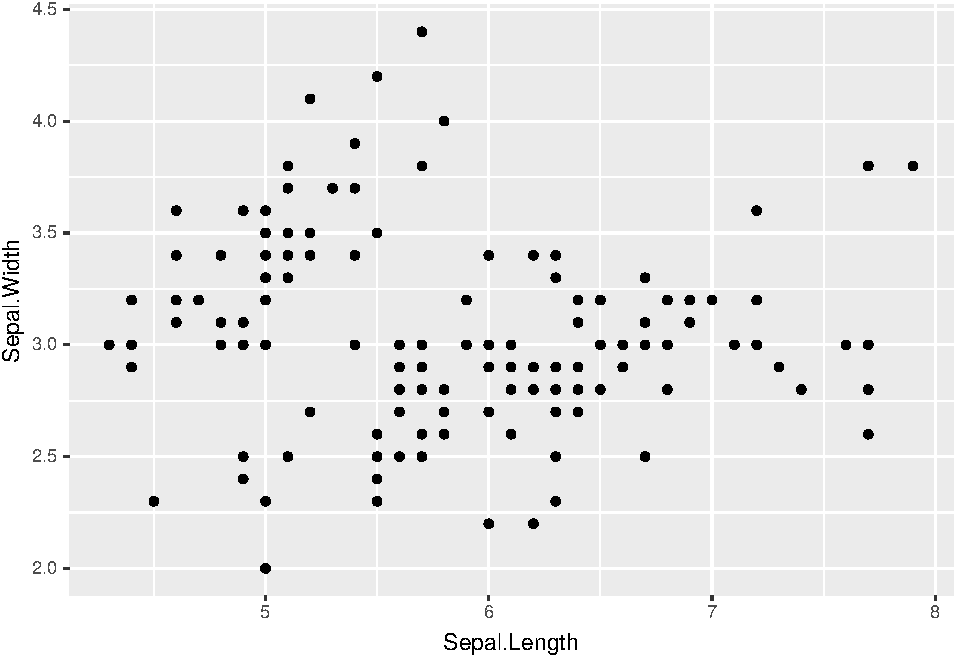
\includegraphics{bookdown-demo_files/figure-latex/unnamed-chunk-51-1.pdf}

In this case the first argument to the \texttt{ggplot} function is the
name of the data frame. Second, the \texttt{aes} (short for aesthetics)
function specifies the mapping to the \texttt{x} and \texttt{y} axes. By
itself the \texttt{ggplot} function as written doesn't tell R what sort
of graphical display is desired. That is done by adding a \texttt{geom}
(short for geometry) specification, in this case \texttt{geom\_point}.

Looking at the scatter plot and thinking about the focus of finding a
method to classify the species, two thoughts come to mind. First, the
plot might be improved by increasing the size of the points. And second,
using different colors for the points corresponding to the three species
would help.

\begin{Shaded}
\begin{Highlighting}[]
\KeywordTok{ggplot}\NormalTok{(}\DataTypeTok{data =}\NormalTok{ iris, }\KeywordTok{aes}\NormalTok{(}\DataTypeTok{x =}\NormalTok{ Sepal.Length, }\DataTypeTok{y =}\NormalTok{ Sepal.Width)) }\OperatorTok{+}\StringTok{ }
\StringTok{    }\KeywordTok{geom_point}\NormalTok{(}\DataTypeTok{size =} \DecValTok{4}\NormalTok{, }\KeywordTok{aes}\NormalTok{(}\DataTypeTok{color=}\NormalTok{Species))}
\end{Highlighting}
\end{Shaded}

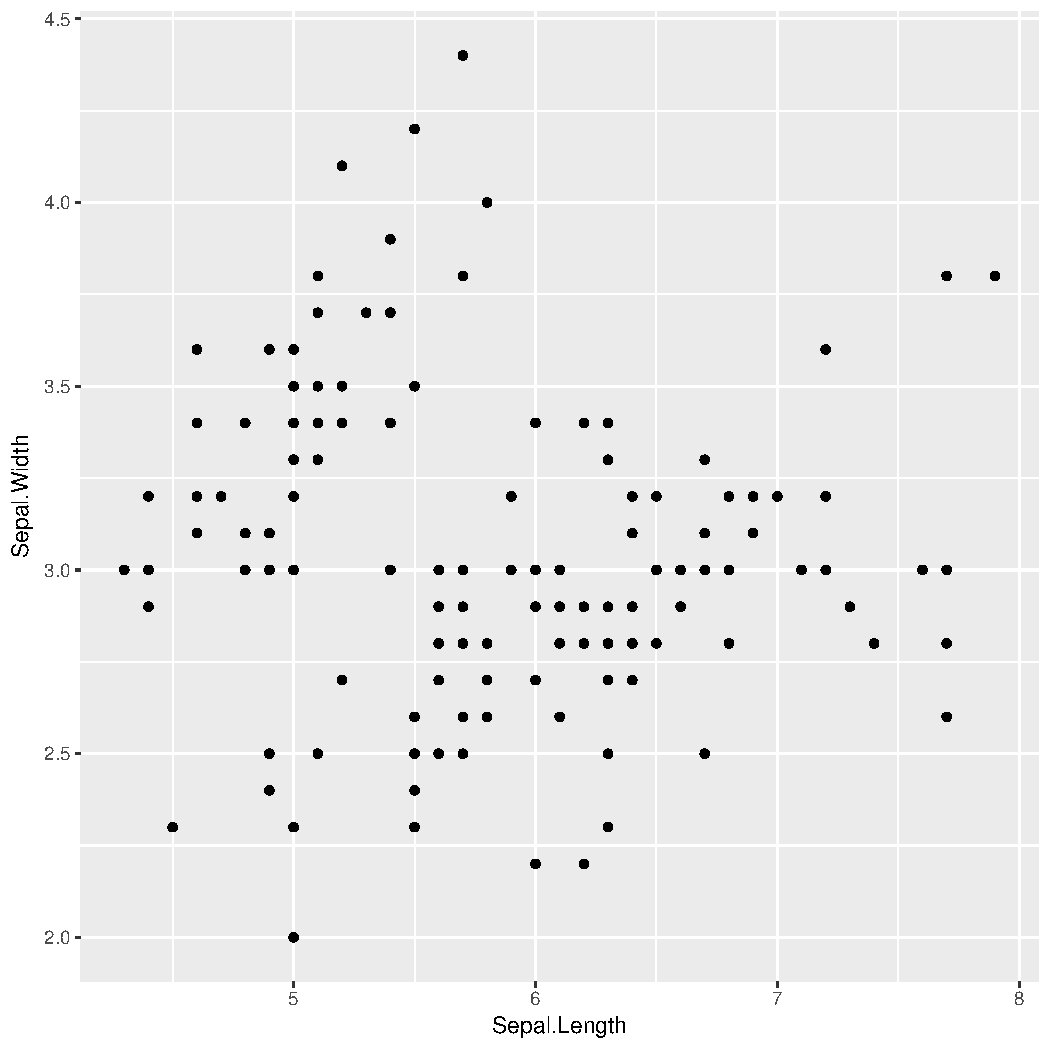
\includegraphics{bookdown-demo_files/figure-latex/unnamed-chunk-52-1.pdf}

Notice that a legend showing what the colors represent is automatically
generated and included in the graphic. Next, the size of the points
seems a bit big now, and it might be helpful to use different shapes for
the different species.

\begin{Shaded}
\begin{Highlighting}[]
\KeywordTok{ggplot}\NormalTok{(}\DataTypeTok{data =}\NormalTok{ iris, }\KeywordTok{aes}\NormalTok{(}\DataTypeTok{x =}\NormalTok{ Sepal.Length, }\DataTypeTok{y =}\NormalTok{ Sepal.Width)) }\OperatorTok{+}\StringTok{ }
\StringTok{    }\KeywordTok{geom_point}\NormalTok{(}\DataTypeTok{size =} \DecValTok{3}\NormalTok{, }\KeywordTok{aes}\NormalTok{(}\DataTypeTok{color=}\NormalTok{Species, }\DataTypeTok{shape=}\NormalTok{Species))}
\end{Highlighting}
\end{Shaded}

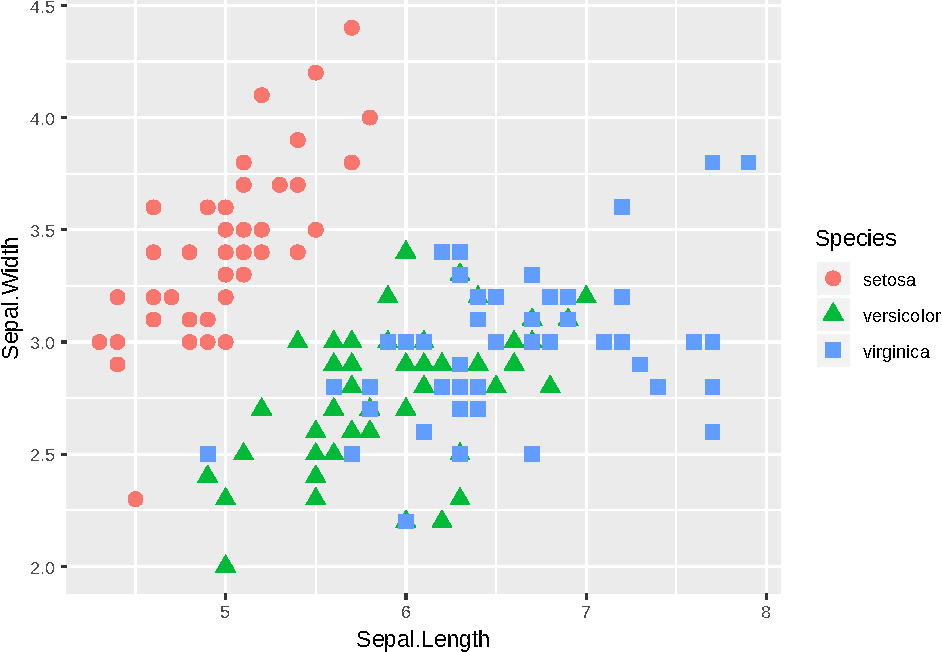
\includegraphics{bookdown-demo_files/figure-latex/unnamed-chunk-53-1.pdf}

Here we see that the legend automatically changes to include species
specific color and shape. The size of the points seems more appropriate.

\subsection{\texorpdfstring{Structure of a Typical
\texttt{ggplot}}{Structure of a Typical ggplot}}\label{structure-of-a-typical-ggplot}

The examples above start with the function \texttt{ggplot()}, which
takes as arguments the data frame containing the data to be plotted as
well as a mapping from the data to the axes, enclosed by the
\texttt{aes()} function. Next a \texttt{geom} function, in the above
case \texttt{geom\_point()}, is added. It might just specify the
geometry, but also might specify aspects such as size, color, or shape.

Typically many graphics are created and discarded in the search for an
informative graphic, and often the initial specification of data and
basic aesthetics from \texttt{ggplot()} stays the same in all the
attempts. In such a case it can be helpful to assign that portion of the
graphic to an R object, both to minimize the amount of typing and to
keep certain aspects of all the graphics constant. Here's how that could
be done for the graphics above.

\begin{Shaded}
\begin{Highlighting}[]
\NormalTok{iris.p <-}\StringTok{ }\KeywordTok{ggplot}\NormalTok{(}\DataTypeTok{data =}\NormalTok{ iris, }\KeywordTok{aes}\NormalTok{(}\DataTypeTok{x =}\NormalTok{ Sepal.Length, }\DataTypeTok{y =}\NormalTok{ Sepal.Width))}
\NormalTok{iris.p }\OperatorTok{+}\StringTok{ }\KeywordTok{geom_point}\NormalTok{()}
\end{Highlighting}
\end{Shaded}

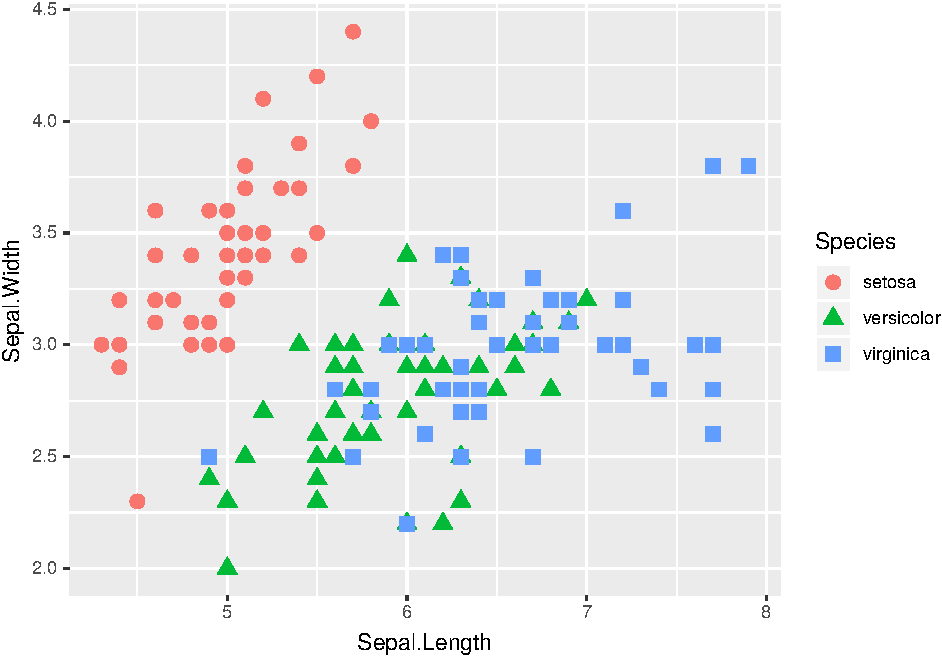
\includegraphics{bookdown-demo_files/figure-latex/unnamed-chunk-54-1.pdf}

\begin{Shaded}
\begin{Highlighting}[]
\NormalTok{iris.p }\OperatorTok{+}\StringTok{ }\KeywordTok{geom_point}\NormalTok{(}\DataTypeTok{size =} \DecValTok{3}\NormalTok{, }\KeywordTok{aes}\NormalTok{(}\DataTypeTok{color =}\NormalTok{ Species, }\DataTypeTok{shape =}\NormalTok{ Species))}
\end{Highlighting}
\end{Shaded}

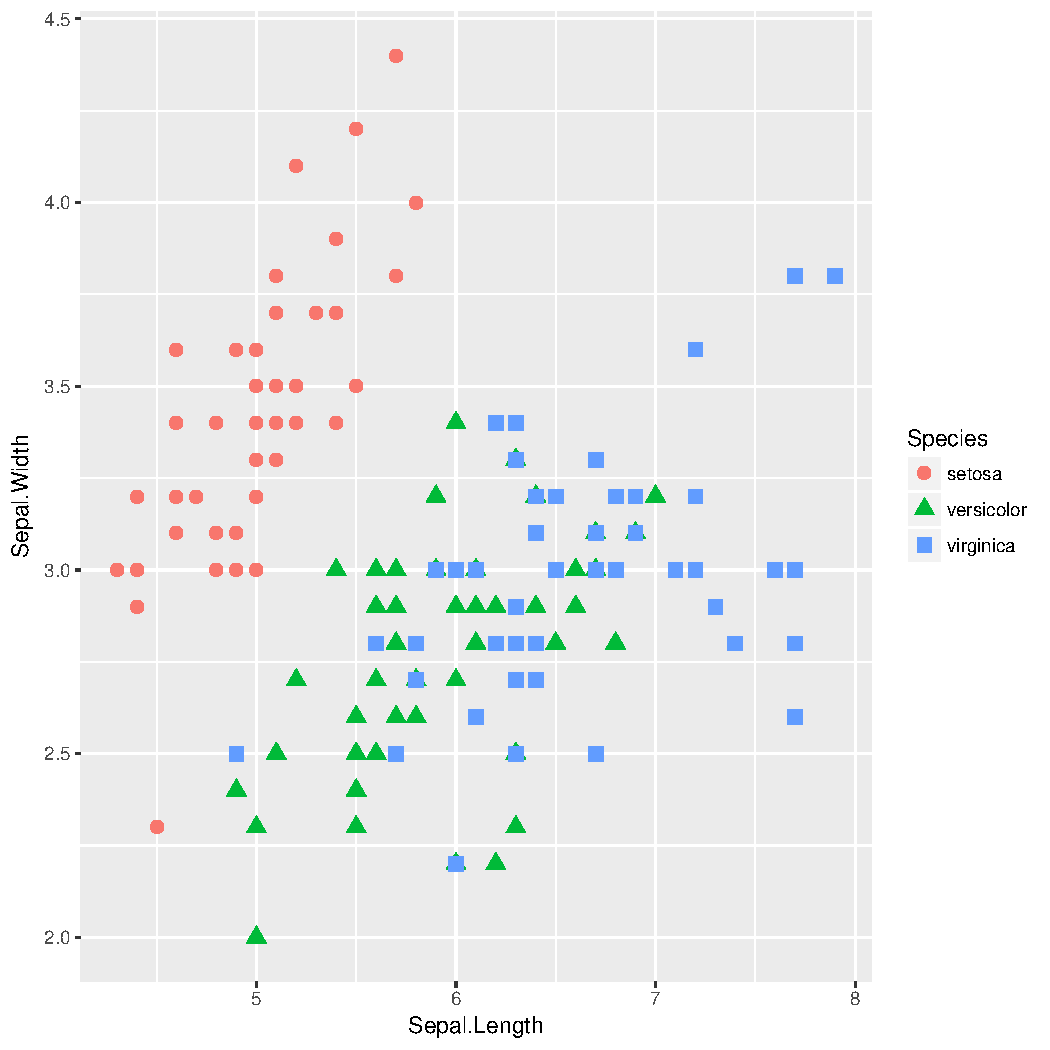
\includegraphics{bookdown-demo_files/figure-latex/unnamed-chunk-54-2.pdf}

\subsection{Adding lines to a scatter
plot}\label{adding-lines-to-a-scatter-plot}

To add a fitted least squares line to a scatter plot, use
\texttt{stat\_smooth}, which adds a smoother (possibly a least squares
line, possibly a smooth curve fit to the data, etc.). The argument
\texttt{method\ =\ lm} specifies a line fitted by least squares, and the
argument \texttt{se\ =\ FALSE} suppresses the default display of a
confidence band around the line or curve which was fit to the data.

\begin{Shaded}
\begin{Highlighting}[]
\KeywordTok{ggplot}\NormalTok{(}\DataTypeTok{data =}\NormalTok{ iris, }\KeywordTok{aes}\NormalTok{(}\DataTypeTok{x =}\NormalTok{ Sepal.Length, }\DataTypeTok{y =}\NormalTok{ Sepal.Width)) }\OperatorTok{+}\StringTok{ }
\StringTok{    }\KeywordTok{geom_point}\NormalTok{(}\DataTypeTok{size=}\DecValTok{3}\NormalTok{, }\KeywordTok{aes}\NormalTok{(}\DataTypeTok{color=}\NormalTok{Species))}
\end{Highlighting}
\end{Shaded}

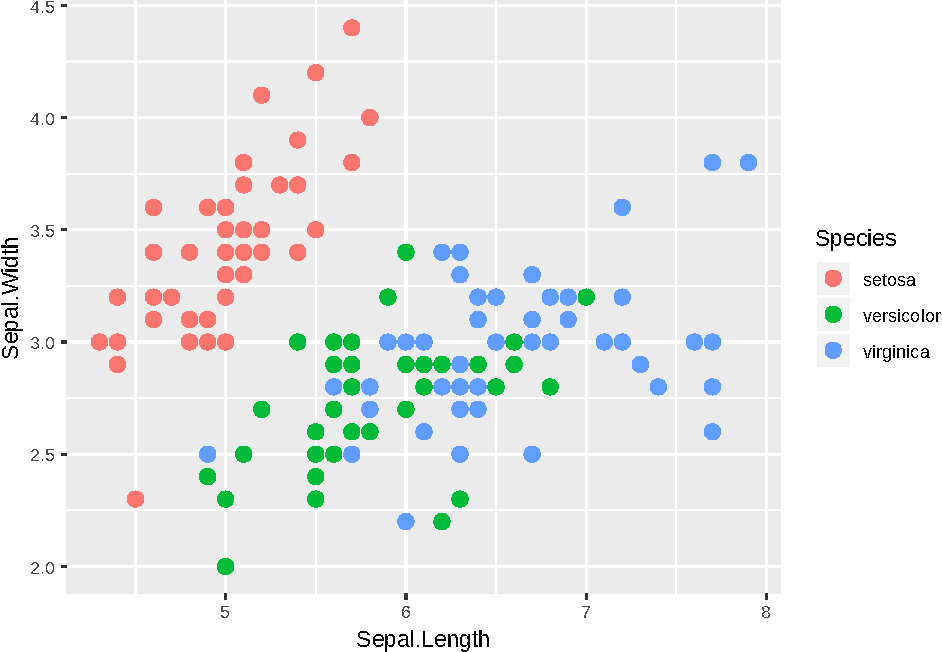
\includegraphics{bookdown-demo_files/figure-latex/unnamed-chunk-55-1.pdf}

\begin{Shaded}
\begin{Highlighting}[]
\KeywordTok{ggplot}\NormalTok{(}\DataTypeTok{data =}\NormalTok{ iris, }\KeywordTok{aes}\NormalTok{(}\DataTypeTok{x =}\NormalTok{ Sepal.Length, }\DataTypeTok{y =}\NormalTok{ Sepal.Width)) }\OperatorTok{+}\StringTok{ }
\StringTok{    }\KeywordTok{geom_point}\NormalTok{(}\DataTypeTok{size=}\DecValTok{3}\NormalTok{, }\KeywordTok{aes}\NormalTok{(}\DataTypeTok{color=}\NormalTok{Species)) }\OperatorTok{+}\StringTok{ }
\StringTok{    }\KeywordTok{stat_smooth}\NormalTok{(}\DataTypeTok{method =}\NormalTok{ lm, }\DataTypeTok{se=}\OtherTok{FALSE}\NormalTok{)}
\end{Highlighting}
\end{Shaded}

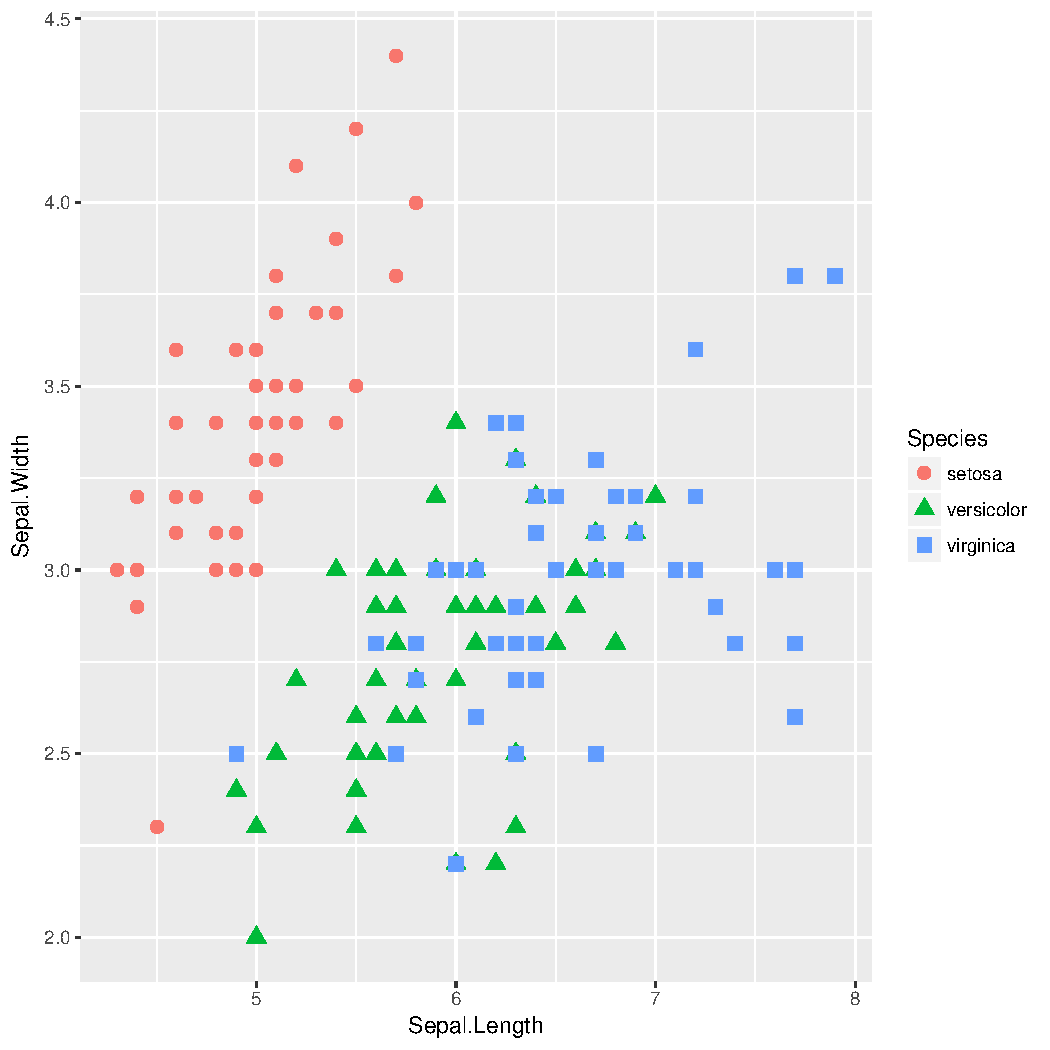
\includegraphics{bookdown-demo_files/figure-latex/unnamed-chunk-55-2.pdf}

For the iris data, it probably makes more sense to fit separate lines by
species. This can be specified using the \texttt{aes()} function inside
\texttt{stat\_smooth()}.

\begin{Shaded}
\begin{Highlighting}[]
\KeywordTok{ggplot}\NormalTok{(}\DataTypeTok{data =}\NormalTok{ iris, }\KeywordTok{aes}\NormalTok{(}\DataTypeTok{x =}\NormalTok{ Sepal.Length, }\DataTypeTok{y =}\NormalTok{ Sepal.Width)) }\OperatorTok{+}\StringTok{ }
\StringTok{    }\KeywordTok{geom_point}\NormalTok{(}\DataTypeTok{size=}\DecValTok{3}\NormalTok{, }\KeywordTok{aes}\NormalTok{(}\DataTypeTok{color=}\NormalTok{Species)) }\OperatorTok{+}\StringTok{ }
\StringTok{    }\KeywordTok{stat_smooth}\NormalTok{(}\DataTypeTok{method =}\NormalTok{ lm, }\DataTypeTok{se=}\OtherTok{FALSE}\NormalTok{, }\KeywordTok{aes}\NormalTok{(}\DataTypeTok{color=}\NormalTok{Species))}
\end{Highlighting}
\end{Shaded}

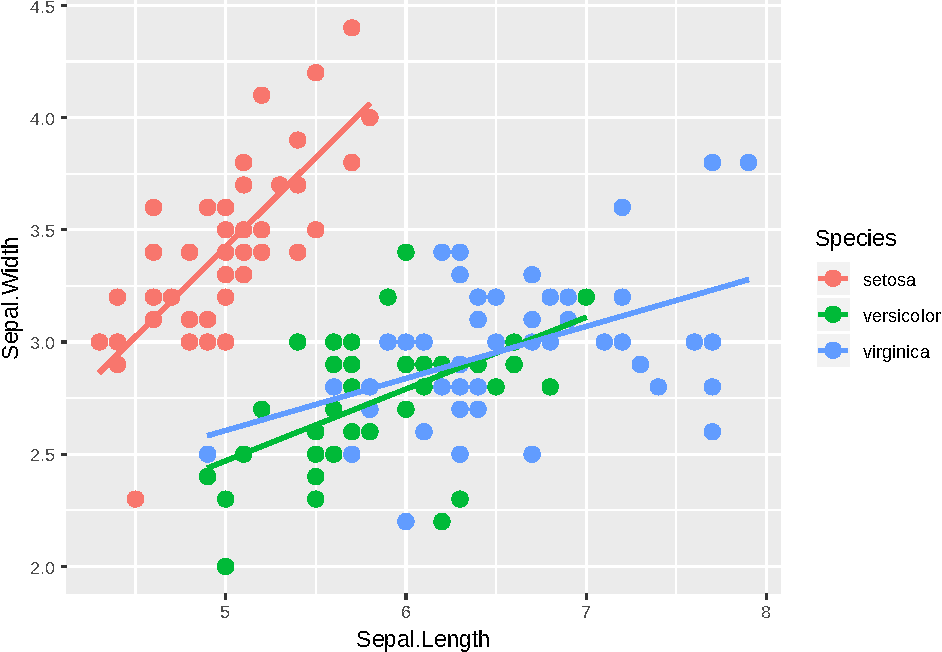
\includegraphics{bookdown-demo_files/figure-latex/unnamed-chunk-56-1.pdf}

In this case we specified the same color aesthetic for the points and
the lines. If we know we want this color aesthetic (colors corresponding
to species) for all aspects of the graphic, we can specify it in the
main \texttt{ggplot()} function:

\begin{Shaded}
\begin{Highlighting}[]
\KeywordTok{ggplot}\NormalTok{(}\DataTypeTok{data =}\NormalTok{ iris, }\KeywordTok{aes}\NormalTok{(}\DataTypeTok{x =}\NormalTok{ Sepal.Length, }\DataTypeTok{y =}\NormalTok{ Sepal.Width, }\DataTypeTok{color =}\NormalTok{ Species)) }\OperatorTok{+}\StringTok{ }
\StringTok{    }\KeywordTok{geom_point}\NormalTok{(}\DataTypeTok{size=}\DecValTok{3}\NormalTok{) }\OperatorTok{+}\StringTok{ }\KeywordTok{stat_smooth}\NormalTok{(}\DataTypeTok{method =}\NormalTok{ lm, }\DataTypeTok{se=}\OtherTok{FALSE}\NormalTok{)}
\end{Highlighting}
\end{Shaded}

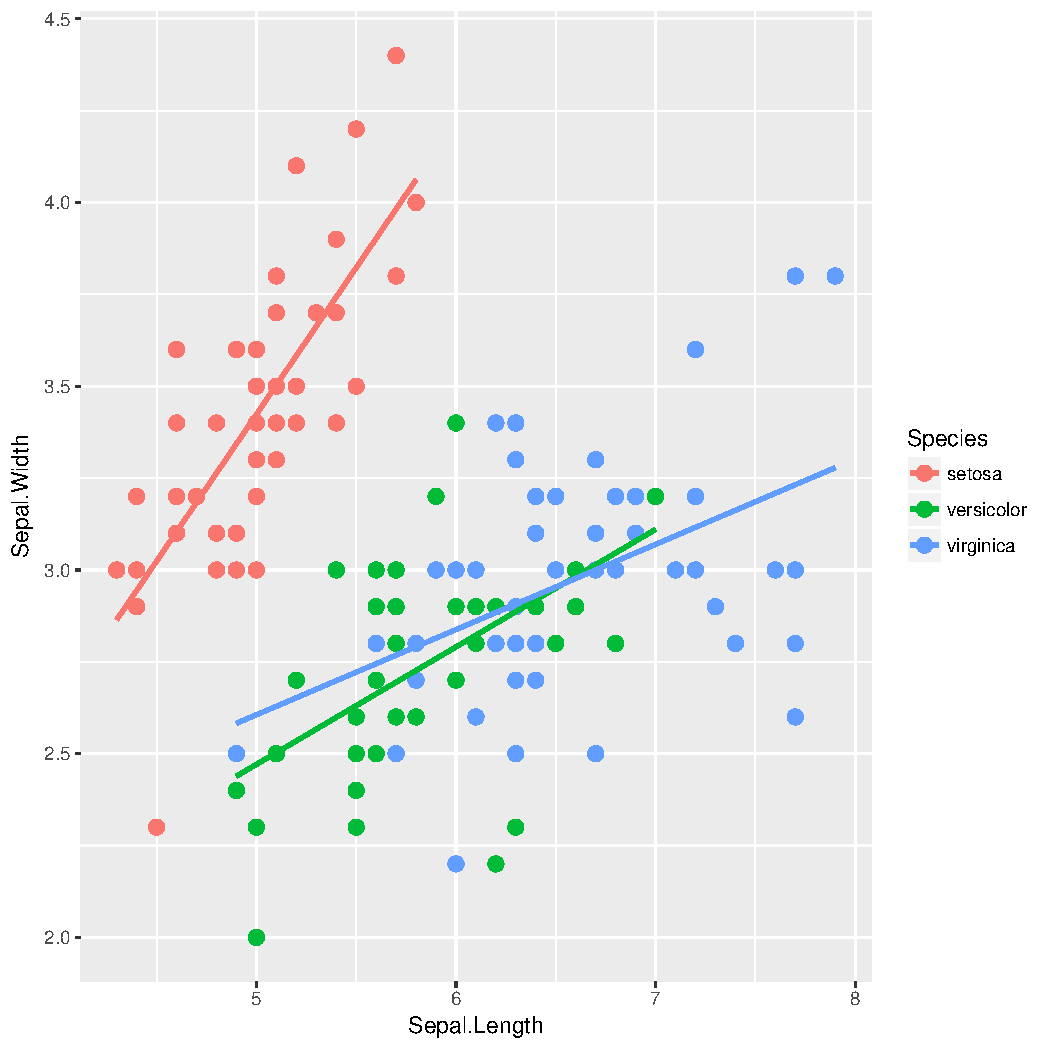
\includegraphics{bookdown-demo_files/figure-latex/unnamed-chunk-57-1.pdf}

Another common use of line segments in a graphic is to connect the
points in order, accomplished via the \texttt{geom\_line()} function.
Although it is not clear why this helps in understanding the iris data,
the technique is illustrated next, first doing this for all the points
in the graphic, and second doing this separately for the three species.

\begin{Shaded}
\begin{Highlighting}[]
\KeywordTok{ggplot}\NormalTok{(}\DataTypeTok{data =}\NormalTok{ iris, }\KeywordTok{aes}\NormalTok{(}\DataTypeTok{x =}\NormalTok{ Sepal.Length, }\DataTypeTok{y =}\NormalTok{ Sepal.Width)) }\OperatorTok{+}\StringTok{ }
\StringTok{    }\KeywordTok{geom_point}\NormalTok{(}\DataTypeTok{size =} \DecValTok{4}\NormalTok{, }\KeywordTok{aes}\NormalTok{(}\DataTypeTok{color=}\NormalTok{Species, }\DataTypeTok{shape =}\NormalTok{ Species)) }\OperatorTok{+}\StringTok{ }
\StringTok{    }\KeywordTok{geom_line}\NormalTok{()}
\end{Highlighting}
\end{Shaded}

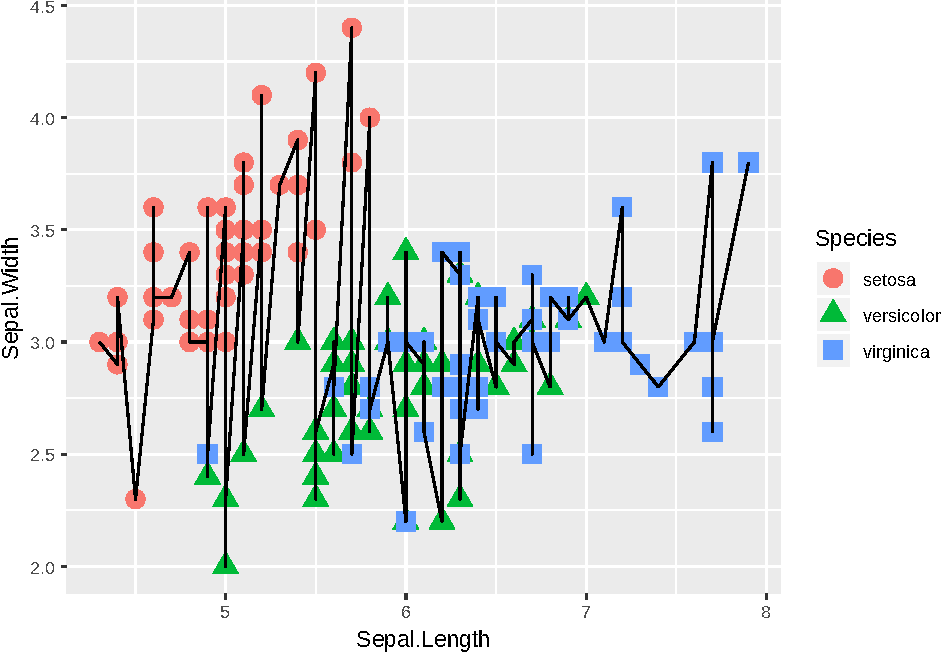
\includegraphics{bookdown-demo_files/figure-latex/unnamed-chunk-58-1.pdf}

\begin{Shaded}
\begin{Highlighting}[]
\KeywordTok{ggplot}\NormalTok{(}\DataTypeTok{data =}\NormalTok{ iris, }\KeywordTok{aes}\NormalTok{(}\DataTypeTok{x =}\NormalTok{ Sepal.Length, }\DataTypeTok{y =}\NormalTok{ Sepal.Width)) }\OperatorTok{+}\StringTok{ }
\StringTok{    }\KeywordTok{geom_point}\NormalTok{(}\DataTypeTok{size =} \DecValTok{4}\NormalTok{, }\KeywordTok{aes}\NormalTok{(}\DataTypeTok{color=}\NormalTok{Species)) }\OperatorTok{+}\StringTok{ }
\StringTok{    }\KeywordTok{geom_line}\NormalTok{(}\KeywordTok{aes}\NormalTok{(}\DataTypeTok{color=}\NormalTok{Species))}
\end{Highlighting}
\end{Shaded}

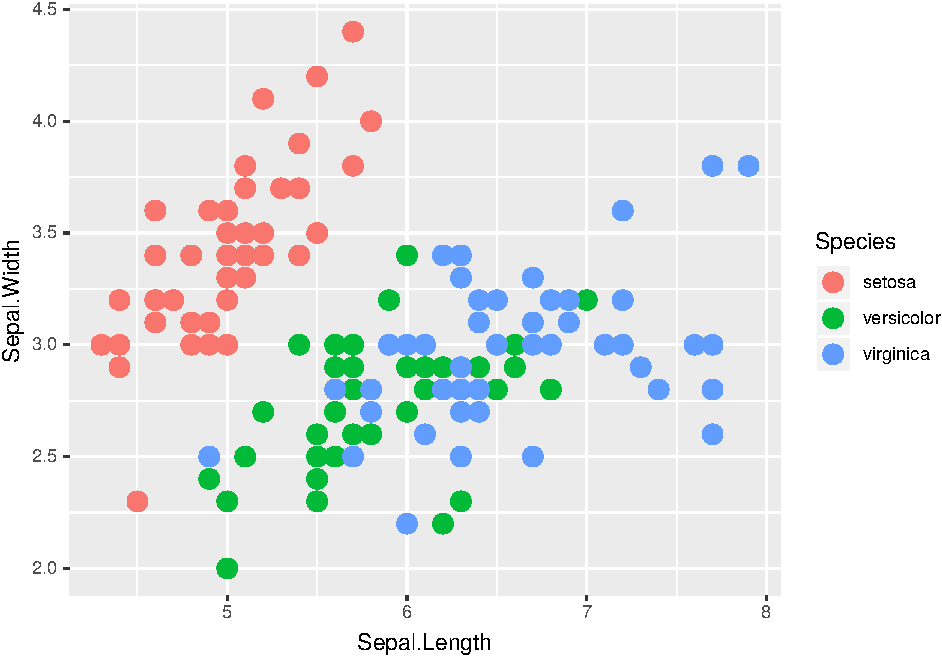
\includegraphics{bookdown-demo_files/figure-latex/unnamed-chunk-59-1.pdf}

\section{Labels, Axes, Text, etc.}\label{labels-axes-text-etc.}

The default settings of \texttt{ggplot2} often produce excellent
graphics, but once a graphic is chosen for dissemination, the user will
likely want to customize things like the title, axes, etc. In this
section some tools for customization are presented. Most will be
illustrated in the context of a data set on crime rates in the 50 states
in the United States. These data were made available by Nathan Yau at
\url{http://flowingdata.com/2010/11/23/how-to-make-bubble-charts/}. The
data include crime rates per 100,000 people for various crimes such as
murder and robbery, and also include each state's population. The crime
rates are from the year 2005, while the population numbers are from the
year 2008, but the difference in population between the years is not
great, and the exact population is not particularly important for what
we'll do below.

First, read in the data, examine its structure, and produce a simple
scatter plot of motor vehicle theft versus burglary.

\begin{Shaded}
\begin{Highlighting}[]
\OperatorTok{>}\StringTok{ }\NormalTok{u.crime <-}\StringTok{ "http://blue.for.msu.edu/FOR875/data/crimeRatesByState2005.csv"}
\OperatorTok{>}\StringTok{ }\NormalTok{crime <-}\StringTok{ }\KeywordTok{read.csv}\NormalTok{(u.crime, }\DataTypeTok{header=}\OtherTok{TRUE}\NormalTok{)}
\OperatorTok{>}\StringTok{ }\KeywordTok{str}\NormalTok{(crime)}
\end{Highlighting}
\end{Shaded}

\begin{verbatim}
'data.frame':   50 obs. of  9 variables:
 $ state              : Factor w/ 50 levels "Alabama ","Alaska ",..: 1 2 3 4 5 6 7 8 9 10 ...
 $ murder             : num  8.2 4.8 7.5 6.7 6.9 3.7 2.9 4.4 5 6.2 ...
 $ Forcible_rate      : num  34.3 81.1 33.8 42.9 26 43.4 20 44.7 37.1 23.6 ...
 $ Robbery            : num  141.4 80.9 144.4 91.1 176.1 ...
 $ aggravated_assult  : num  248 465 327 387 317 ...
 $ burglary           : num  954 622 948 1085 693 ...
 $ larceny_theft      : num  2650 2599 2965 2711 1916 ...
 $ motor_vehicle_theft: num  288 391 924 262 713 ...
 $ population         : int  4627851 686293 6500180 2855390 36756666 4861515 3501252 873092 18328340 9685744 ...
\end{verbatim}

\begin{Shaded}
\begin{Highlighting}[]
\OperatorTok{>}\StringTok{ }\KeywordTok{ggplot}\NormalTok{(data <-}\StringTok{ }\NormalTok{crime, }\KeywordTok{aes}\NormalTok{(}\DataTypeTok{x =}\NormalTok{ burglary, }\DataTypeTok{y =}\NormalTok{ motor_vehicle_theft)) }\OperatorTok{+}\StringTok{ }
\OperatorTok{+}\StringTok{     }\KeywordTok{geom_point}\NormalTok{()}
\end{Highlighting}
\end{Shaded}

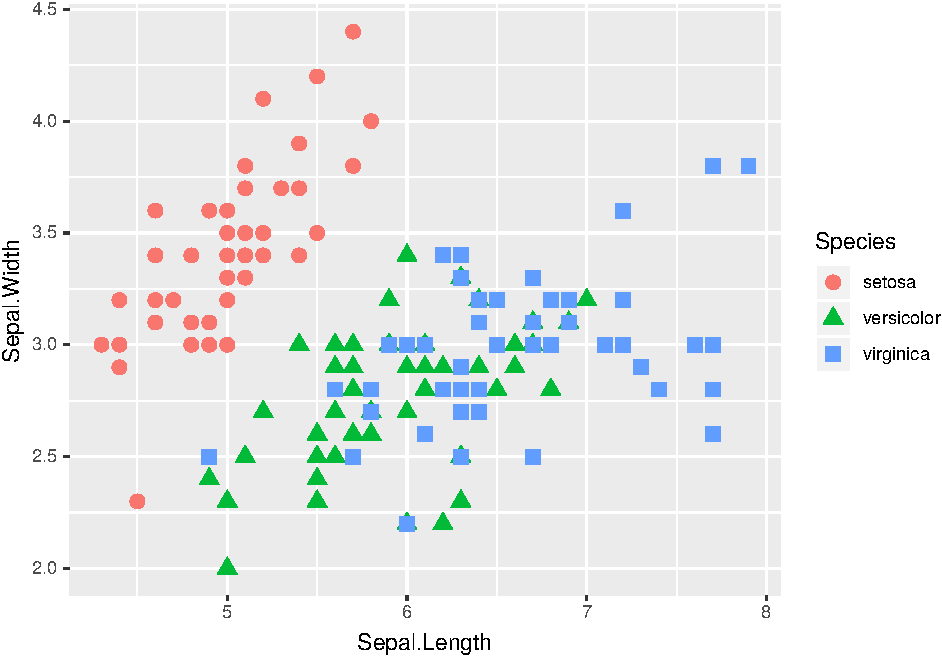
\includegraphics{bookdown-demo_files/figure-latex/unnamed-chunk-60-1.pdf}

\subsection{Labels}\label{labels}

By default axis and legend labels are the names of the relevant columns
in the data frame. While convenient, we often want to customize these
labels. Here we use \texttt{labs()} to change the x and y axis labels
and other descriptive text.\footnote{Axis and legend labels can also be
  set in the individual scales, see the subsequent sections.}

\begin{Shaded}
\begin{Highlighting}[]
\KeywordTok{ggplot}\NormalTok{(}\DataTypeTok{data =}\NormalTok{ crime, }\KeywordTok{aes}\NormalTok{(}\DataTypeTok{x =}\NormalTok{ burglary, }\DataTypeTok{y =}\NormalTok{ motor_vehicle_theft)) }\OperatorTok{+}\StringTok{ }
\StringTok{    }\KeywordTok{geom_point}\NormalTok{() }\OperatorTok{+}\StringTok{ }
\StringTok{    }\KeywordTok{labs}\NormalTok{(}\DataTypeTok{x =} \StringTok{"Burglaries per 100,000 population"}\NormalTok{, }
         \DataTypeTok{y =} \StringTok{"Motor vehicle theft per 100,000 population"}\NormalTok{,}
         \DataTypeTok{title =} \StringTok{"Burglaries vs motor vehicle theft for US states"}\NormalTok{,}
         \DataTypeTok{subtitle =} \StringTok{"2005 crime rates and 2008 population"}\NormalTok{,}
         \DataTypeTok{caption =} \StringTok{"Data from Nathan Yau http://flowingdata.com"}
\NormalTok{         )}
\end{Highlighting}
\end{Shaded}

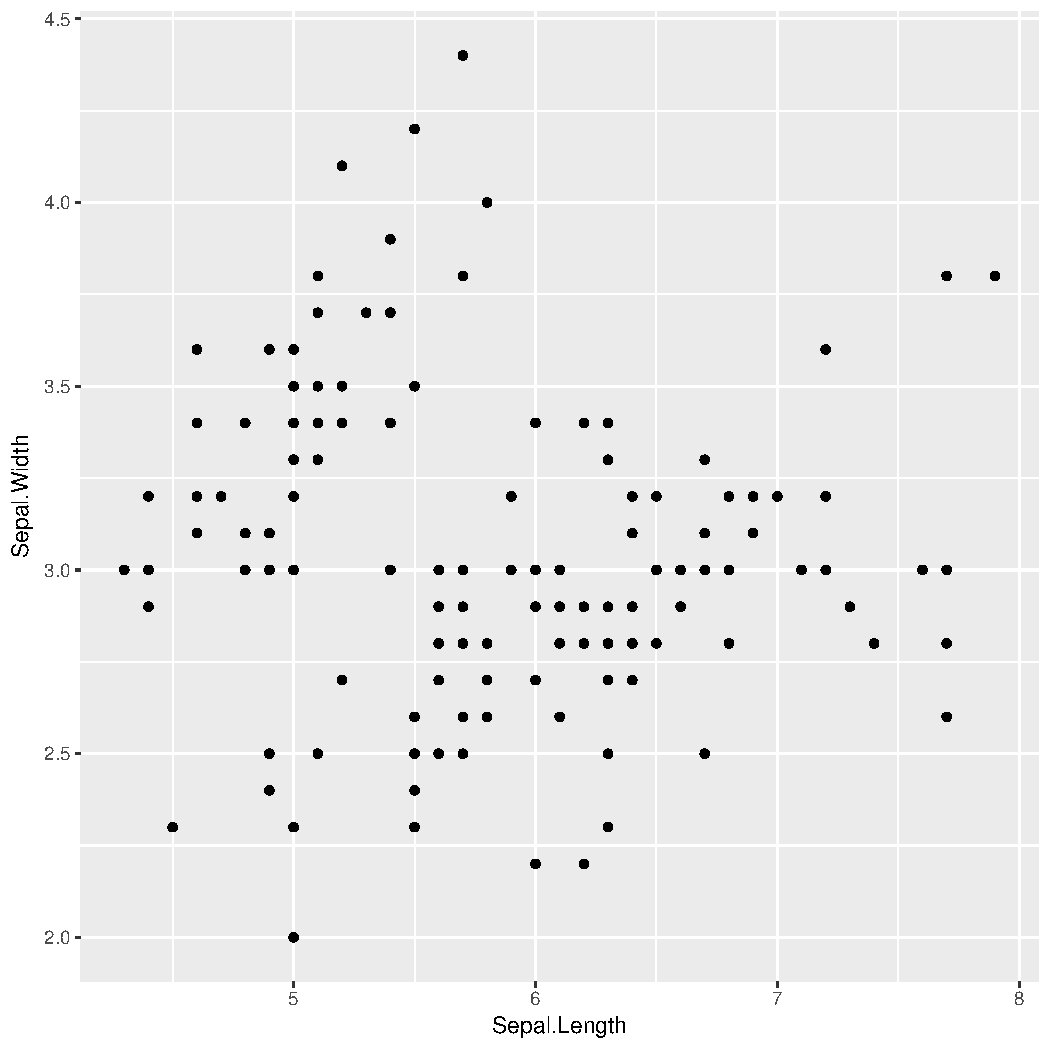
\includegraphics{bookdown-demo_files/figure-latex/unnamed-chunk-61-1.pdf}

\chapter{Customizing Axes}\label{customizing-axes}

\texttt{ggplot} also provides default axis extents (i.e., limits) and
other axis features. These, and other axis features such as tick marks,
labels, and transformations, can be changed using the scale functions.
Here the range of the x and y axis is altered to start at zero and go to
the maximum of the x and y variables.\footnote{\texttt{ggplot2} makes
  the axes extend slightly beyond the given range, since typically this
  is what the user wants.} Here too, axis labels are specified within
the scale function, which is an alterative to using the \texttt{labs()}
function.

\begin{Shaded}
\begin{Highlighting}[]
\KeywordTok{ggplot}\NormalTok{(}\DataTypeTok{data =}\NormalTok{ crime, }\KeywordTok{aes}\NormalTok{(}\DataTypeTok{x =}\NormalTok{ burglary, }\DataTypeTok{y =}\NormalTok{ motor_vehicle_theft)) }\OperatorTok{+}\StringTok{ }
\StringTok{    }\KeywordTok{geom_point}\NormalTok{() }\OperatorTok{+}\StringTok{ }
\StringTok{    }\KeywordTok{scale_x_continuous}\NormalTok{(}\DataTypeTok{name=}\StringTok{"Burglaries per 100,000 population"}\NormalTok{, }
                       \DataTypeTok{limits=}\KeywordTok{c}\NormalTok{(}\DecValTok{0}\NormalTok{,}\KeywordTok{max}\NormalTok{(crime}\OperatorTok{$}\NormalTok{burglary))) }\OperatorTok{+}
\StringTok{    }\KeywordTok{scale_y_continuous}\NormalTok{(}\DataTypeTok{name=}\StringTok{"Motor vehicle theft per 100,000 population"}\NormalTok{, }
                       \DataTypeTok{limits =} \KeywordTok{c}\NormalTok{(}\DecValTok{0}\NormalTok{, }\KeywordTok{max}\NormalTok{(crime}\OperatorTok{$}\NormalTok{motor_vehicle_theft)))}
\end{Highlighting}
\end{Shaded}

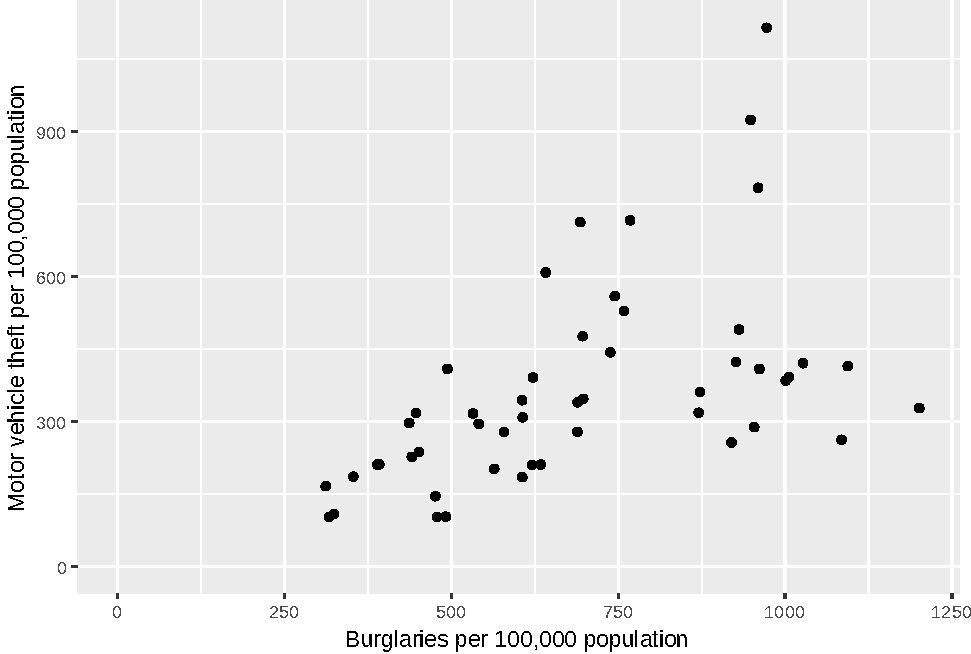
\includegraphics{bookdown-demo_files/figure-latex/unnamed-chunk-62-1.pdf}

\subsection{Text, Point Size, and
Color}\label{text-point-size-and-color}

Next we make point size proportional to population, change the color,
and add a state label. Note, in the \texttt{ggplot()} call I scaled
\texttt{population} by 100,000 to help with the interpretability of the
legend. Accordingly, I also changed the ``population'' label on the
legend to ``Population\n(100,000)'' using the \texttt{labs()}
function\footnote{The \n is the line break and puts ``(100,000)'' below
  ``Population''.}. We use the \texttt{geom\_label()} function to add
the label, which provides an outline around the label text and allows
you to control the box characteristics, e.g., I make the boxes slightly
transparent using the \texttt{alpha} argument.\footnote{You can also add
  labels via \texttt{geom\_text()} function or a \texttt{label} argument
  in the \texttt{ggplot()} call.}

\begin{Shaded}
\begin{Highlighting}[]
\KeywordTok{ggplot}\NormalTok{(}\DataTypeTok{data =}\NormalTok{ crime, }\KeywordTok{aes}\NormalTok{(}\DataTypeTok{x =}\NormalTok{ burglary, }\DataTypeTok{y =}\NormalTok{ motor_vehicle_theft, }
           \DataTypeTok{size=}\NormalTok{population}\OperatorTok{/}\DecValTok{100000}\NormalTok{)) }\OperatorTok{+}\StringTok{ }
\StringTok{    }\KeywordTok{geom_point}\NormalTok{(}\DataTypeTok{color =} \StringTok{"blue"}\NormalTok{) }\OperatorTok{+}\StringTok{ }
\StringTok{    }\KeywordTok{geom_label}\NormalTok{(}\KeywordTok{aes}\NormalTok{(}\DataTypeTok{label =}\NormalTok{ state), }\DataTypeTok{alpha =} \FloatTok{0.5}\NormalTok{) }\OperatorTok{+}
\StringTok{    }\KeywordTok{scale_x_continuous}\NormalTok{(}\DataTypeTok{name=}\StringTok{"Burglaries per 100,000 population"}\NormalTok{, }
                       \DataTypeTok{limits=}\KeywordTok{c}\NormalTok{(}\DecValTok{0}\NormalTok{,}\KeywordTok{max}\NormalTok{(crime}\OperatorTok{$}\NormalTok{burglary))) }\OperatorTok{+}
\StringTok{    }\KeywordTok{scale_y_continuous}\NormalTok{(}\DataTypeTok{name=}\StringTok{"Motor vehicle theft per 100,000 population"}\NormalTok{, }
                       \DataTypeTok{limits =} \KeywordTok{c}\NormalTok{(}\DecValTok{0}\NormalTok{, }\KeywordTok{max}\NormalTok{(crime}\OperatorTok{$}\NormalTok{motor_vehicle_theft))) }\OperatorTok{+}
\StringTok{    }\KeywordTok{labs}\NormalTok{(}\DataTypeTok{size=}\StringTok{"Population}\CharTok{\textbackslash{}n}\StringTok{(100,000)"}\NormalTok{)}
\end{Highlighting}
\end{Shaded}

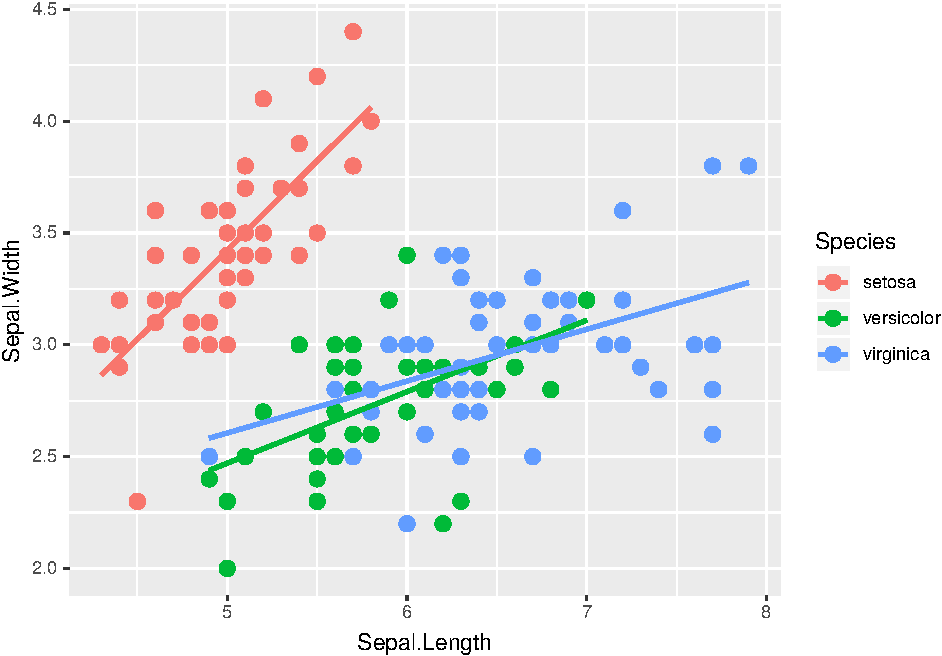
\includegraphics{bookdown-demo_files/figure-latex/unnamed-chunk-63-1.pdf}

The labels are helpful but just too cluttered. There are some additional
arguments that can go into \texttt{geom\_label()} that allow for label
offset; however, this won't help us much here. Instead, we can try the
\texttt{ggrepel} package by Kamil Slowikowski. This useful package will
automatically adjust labels so that they don't overlap. First we need to
download and add the package using either RStudio's install package
buttons or via \texttt{install.packages("ggrepel")}. Next to make all of
\texttt{ggrepel}'s functions available we can call
\texttt{library(ggrepel)} function or, if we know which function we
want, we can load only that particular function using the \texttt{::}
operators. I use \texttt{::} below to make clear which function is
coming from \texttt{ggrepel} and which is coming from \texttt{ggplot2}.

\begin{Shaded}
\begin{Highlighting}[]
\KeywordTok{ggplot}\NormalTok{(}\DataTypeTok{data =}\NormalTok{ crime, }\KeywordTok{aes}\NormalTok{(}\DataTypeTok{x =}\NormalTok{ burglary, }\DataTypeTok{y =}\NormalTok{ motor_vehicle_theft, }
           \DataTypeTok{size=}\NormalTok{population}\OperatorTok{/}\DecValTok{100000}\NormalTok{)) }\OperatorTok{+}\StringTok{ }
\StringTok{    }\KeywordTok{geom_point}\NormalTok{(}\DataTypeTok{color =} \StringTok{"blue"}\NormalTok{) }\OperatorTok{+}\StringTok{ }
\StringTok{    }\KeywordTok{scale_x_continuous}\NormalTok{(}\DataTypeTok{name=}\StringTok{"Burglaries per 100,000 population"}\NormalTok{, }
                       \DataTypeTok{limits=}\KeywordTok{c}\NormalTok{(}\DecValTok{0}\NormalTok{,}\KeywordTok{max}\NormalTok{(crime}\OperatorTok{$}\NormalTok{burglary))) }\OperatorTok{+}
\StringTok{    }\KeywordTok{scale_y_continuous}\NormalTok{(}\DataTypeTok{name=}\StringTok{"Motor vehicle theft per 100,000 population"}\NormalTok{, }
                       \DataTypeTok{limits =} \KeywordTok{c}\NormalTok{(}\DecValTok{0}\NormalTok{, }\KeywordTok{max}\NormalTok{(crime}\OperatorTok{$}\NormalTok{motor_vehicle_theft))) }\OperatorTok{+}
\StringTok{    }\KeywordTok{labs}\NormalTok{(}\DataTypeTok{size=}\StringTok{"Population}\CharTok{\textbackslash{}n}\StringTok{(100,000)"}\NormalTok{) }\OperatorTok{+}
\StringTok{    }\NormalTok{ggrepel}\OperatorTok{::}\KeywordTok{geom_label_repel}\NormalTok{(}\KeywordTok{aes}\NormalTok{(}\DataTypeTok{label =}\NormalTok{ state), }\DataTypeTok{alpha =} \FloatTok{0.5}\NormalTok{)}
\end{Highlighting}
\end{Shaded}

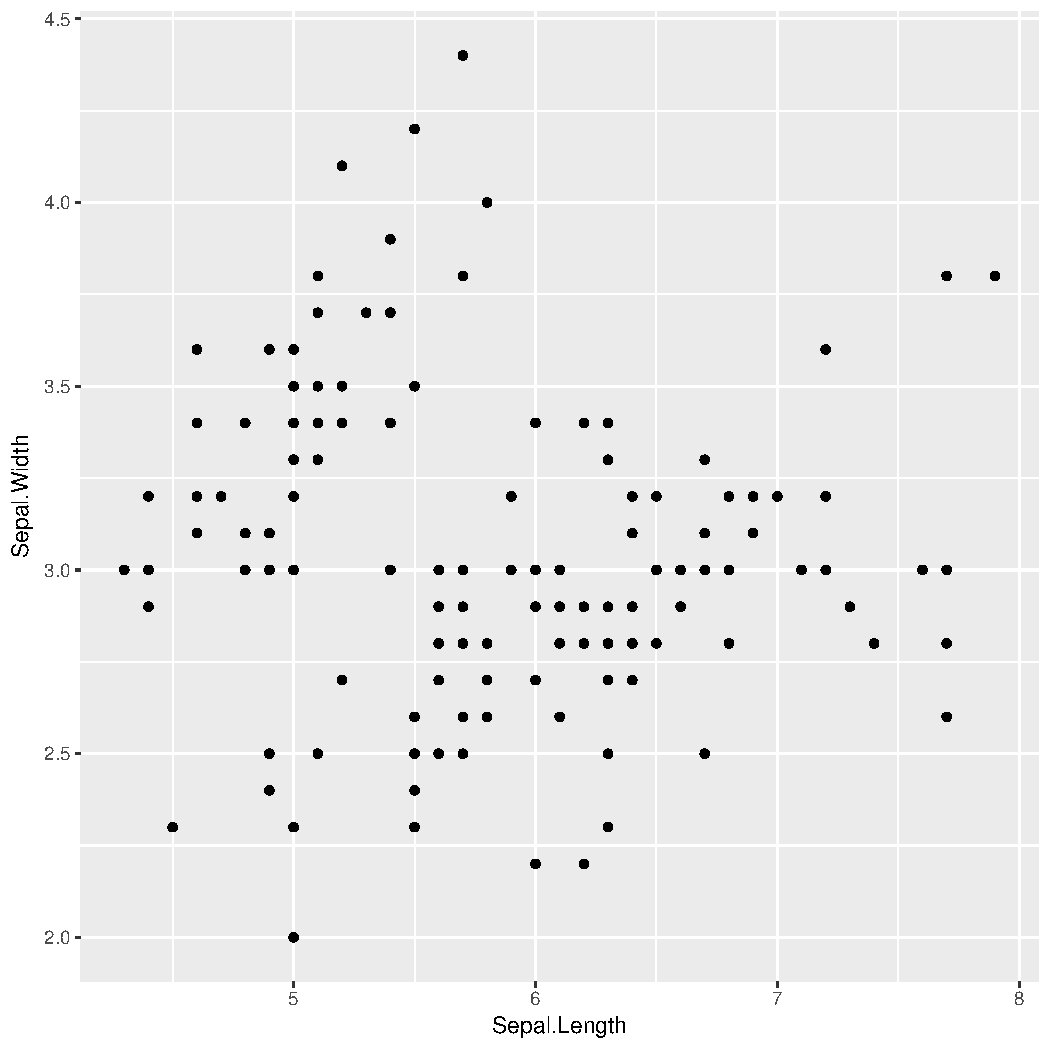
\includegraphics{bookdown-demo_files/figure-latex/unnamed-chunk-64-1.pdf}

This looks a bit better. We'll resist making additional improvements to
the figure for now.

\section{Other Types of Graphics}\label{other-types-of-graphics}

Scatter and line plots, which have just been presented, are common but
certainly not the only graphical displays in common use. Histograms,
boxplots, and bar graphs, as well as more ``mathematical'' displays such
as the graph of a function, are commonly used to represent data.
Examples of each are presented below.

\subsection{Histograms}\label{histograms}

Simon Newcomb conducted several experiments to estimate the speed of
light by measuring the time it took for light to travel from his
laboratory to a mirror at the base of the Washington Monument, and then
back to his lab. This is a distance of \(7.44373\) km, and by dividing
this distance by the measured time, an estimate for the speed of light
is obtained.

The times are of course quite small, and to avoid working with very
small numbers, the data are recoded to be the deviation from \(24800\)
nanoseconds. For example an observation coded as \(28\) represents a
time of \(24828\) nanoseconds, while an observation coded as \(-44\)
represents a time of \(24756\) nanoseconds.

\begin{Shaded}
\begin{Highlighting}[]
\OperatorTok{>}\StringTok{ }\NormalTok{u.newcomb <-}\StringTok{ "http://blue.for.msu.edu/FOR875/data/Newcomb.csv"}
\OperatorTok{>}\StringTok{ }\NormalTok{Newcomb <-}\StringTok{ }\KeywordTok{read.csv}\NormalTok{(u.newcomb, }\DataTypeTok{header =} \OtherTok{TRUE}\NormalTok{)}
\OperatorTok{>}\StringTok{ }\KeywordTok{head}\NormalTok{(Newcomb)}
\end{Highlighting}
\end{Shaded}

\begin{verbatim}
  Time
1   28
2   26
3   33
4   24
5   34
6  -44
\end{verbatim}

\begin{Shaded}
\begin{Highlighting}[]
\KeywordTok{ggplot}\NormalTok{(Newcomb, }\KeywordTok{aes}\NormalTok{(}\DataTypeTok{x =}\NormalTok{ Time)) }\OperatorTok{+}\StringTok{ }\KeywordTok{geom_histogram}\NormalTok{()}
\end{Highlighting}
\end{Shaded}

\begin{verbatim}
`stat_bin()` using `bins = 30`. Pick better value
with `binwidth`.
\end{verbatim}

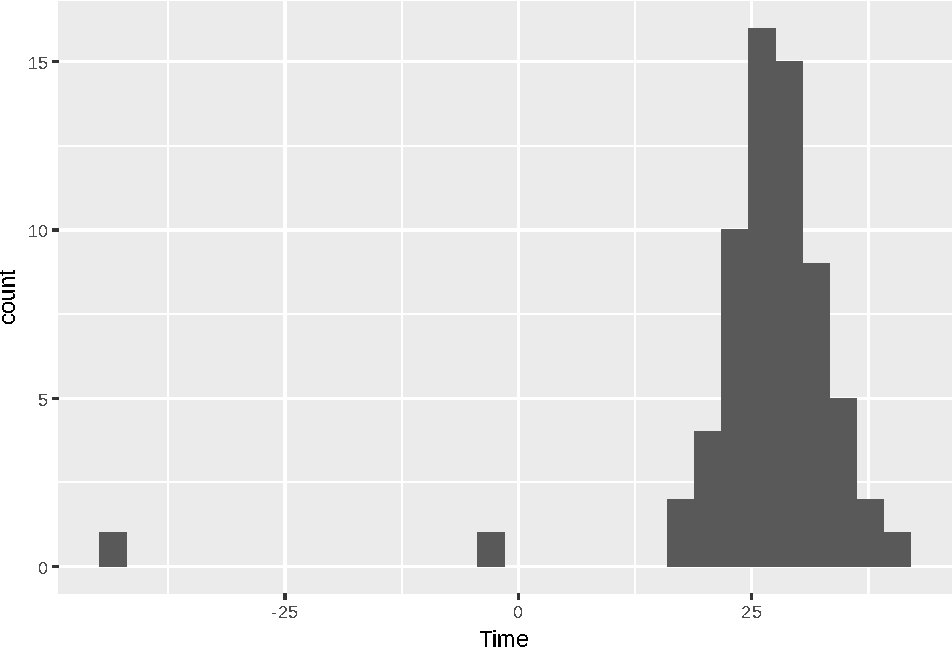
\includegraphics{bookdown-demo_files/figure-latex/unnamed-chunk-66-1.pdf}

The software has an algorithm to calculate bin widths for the histogram.
Sometimes the algorithm makes choices that aren't suitable (hence the R
message above), and these can be changed by specifying a
\texttt{binwidth}. In addition, the appearance of the bars also can be
changed.

\begin{Shaded}
\begin{Highlighting}[]
\KeywordTok{ggplot}\NormalTok{(Newcomb, }\KeywordTok{aes}\NormalTok{(}\DataTypeTok{x =}\NormalTok{ Time)) }\OperatorTok{+}\StringTok{ }
\StringTok{    }\KeywordTok{geom_histogram}\NormalTok{(}\DataTypeTok{binwidth =} \DecValTok{5}\NormalTok{, }\DataTypeTok{color =} \StringTok{"black"}\NormalTok{, }\DataTypeTok{fill =} \StringTok{"blue"}\NormalTok{ )}
\end{Highlighting}
\end{Shaded}

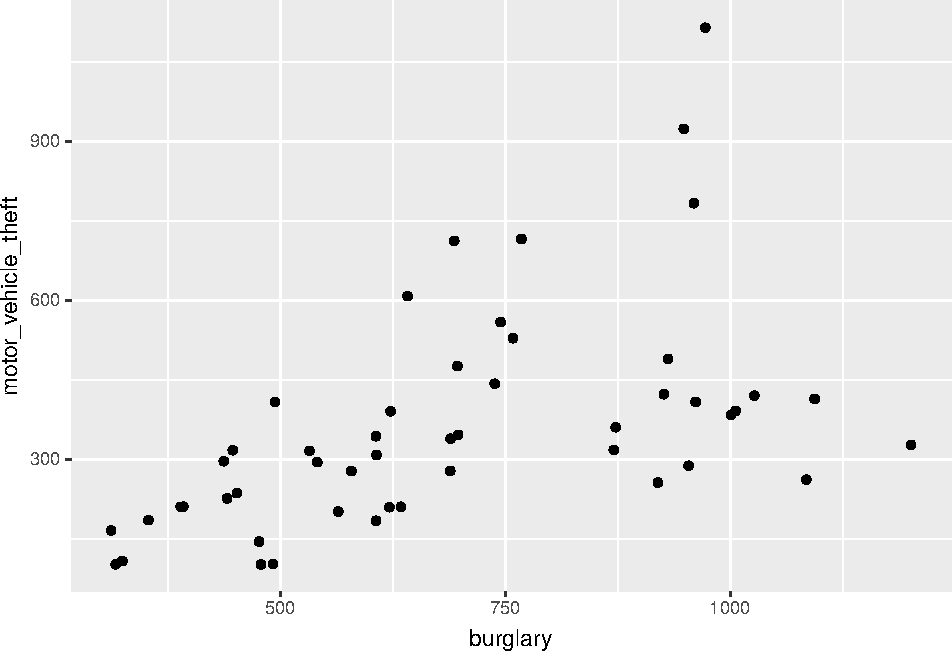
\includegraphics{bookdown-demo_files/figure-latex/unnamed-chunk-67-1.pdf}

\subsection{Boxplots}\label{boxplots}

Next we consider some data from the gap minder data set to construct
some box plots. These data are available in the \texttt{gapminder}
package, which might need to be installed via
\texttt{install.packages("gapminder")}.

\begin{Shaded}
\begin{Highlighting}[]
\KeywordTok{library}\NormalTok{(gapminder)}
\KeywordTok{ggplot}\NormalTok{(}\DataTypeTok{data =} \KeywordTok{subset}\NormalTok{(gapminder,  year }\OperatorTok{==}\StringTok{ }\DecValTok{2002}\NormalTok{), }
       \KeywordTok{aes}\NormalTok{(}\DataTypeTok{x =}\NormalTok{ continent, }\DataTypeTok{y =}\NormalTok{ gdpPercap)) }\OperatorTok{+}\StringTok{ }
\StringTok{    }\KeywordTok{geom_boxplot}\NormalTok{(}\DataTypeTok{color =} \StringTok{"black"}\NormalTok{, }\DataTypeTok{fill =} \StringTok{"lightblue"}\NormalTok{)}
\end{Highlighting}
\end{Shaded}

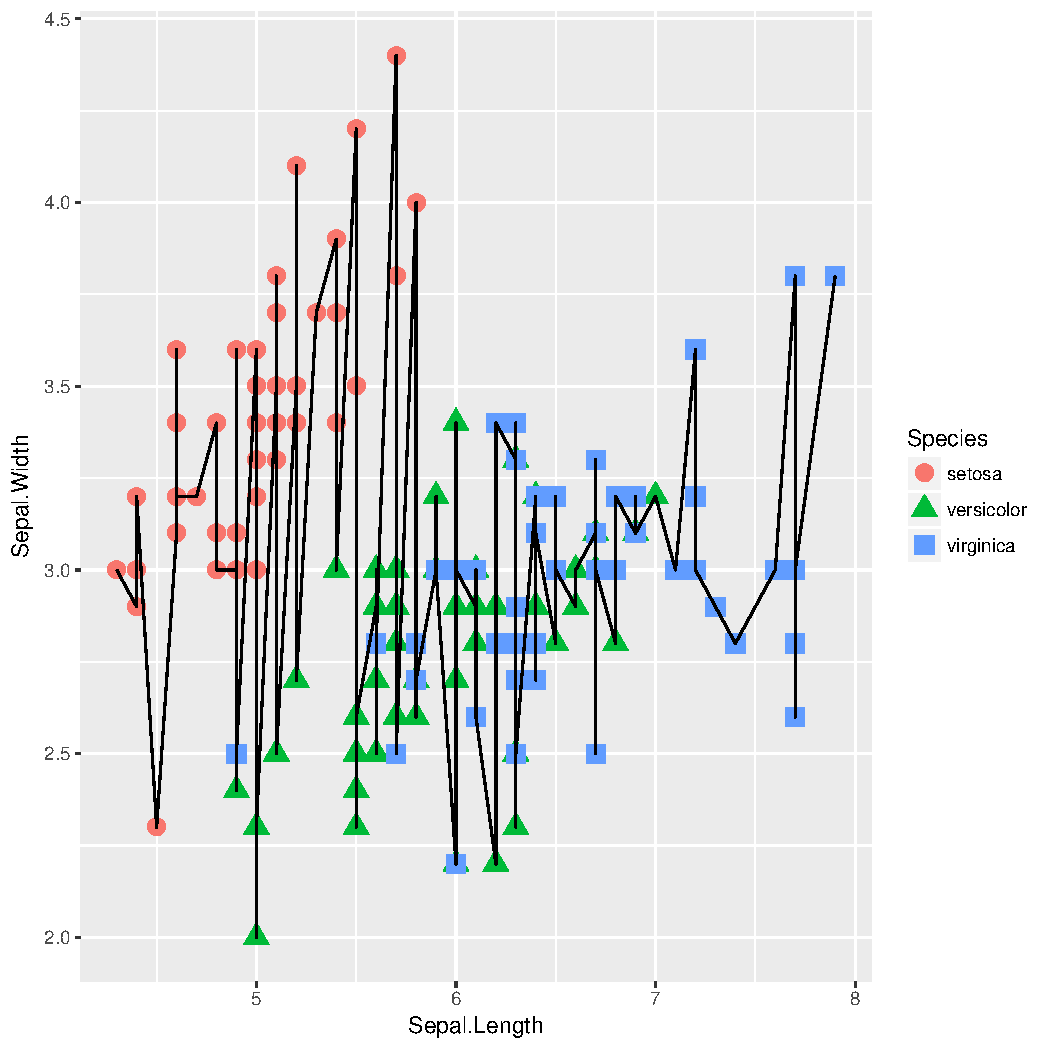
\includegraphics{bookdown-demo_files/figure-latex/unnamed-chunk-68-1.pdf}

Here's the same set of boxplots, but with different colors, different
axis labels, and the boxes plotted horizontally rather than vertically.

\begin{Shaded}
\begin{Highlighting}[]
\KeywordTok{ggplot}\NormalTok{(}\DataTypeTok{data =} \KeywordTok{subset}\NormalTok{(gapminder,  year }\OperatorTok{==}\StringTok{ }\DecValTok{2002}\NormalTok{), }
       \KeywordTok{aes}\NormalTok{(}\DataTypeTok{x =}\NormalTok{ continent, }\DataTypeTok{y =}\NormalTok{ gdpPercap)) }\OperatorTok{+}\StringTok{ }
\StringTok{    }\KeywordTok{geom_boxplot}\NormalTok{(}\DataTypeTok{color =} \StringTok{"red"}\NormalTok{, }\DataTypeTok{fill =} \StringTok{"lightblue"}\NormalTok{) }\OperatorTok{+}\StringTok{ }
\StringTok{    }\KeywordTok{scale_x_discrete}\NormalTok{(}\DataTypeTok{name =} \StringTok{"Continent"}\NormalTok{) }\OperatorTok{+}\StringTok{ }
\StringTok{    }\KeywordTok{scale_y_continuous}\NormalTok{(}\DataTypeTok{name =} \StringTok{"Per Capita GDP"}\NormalTok{) }\OperatorTok{+}\StringTok{ }\KeywordTok{coord_flip}\NormalTok{()}
\end{Highlighting}
\end{Shaded}

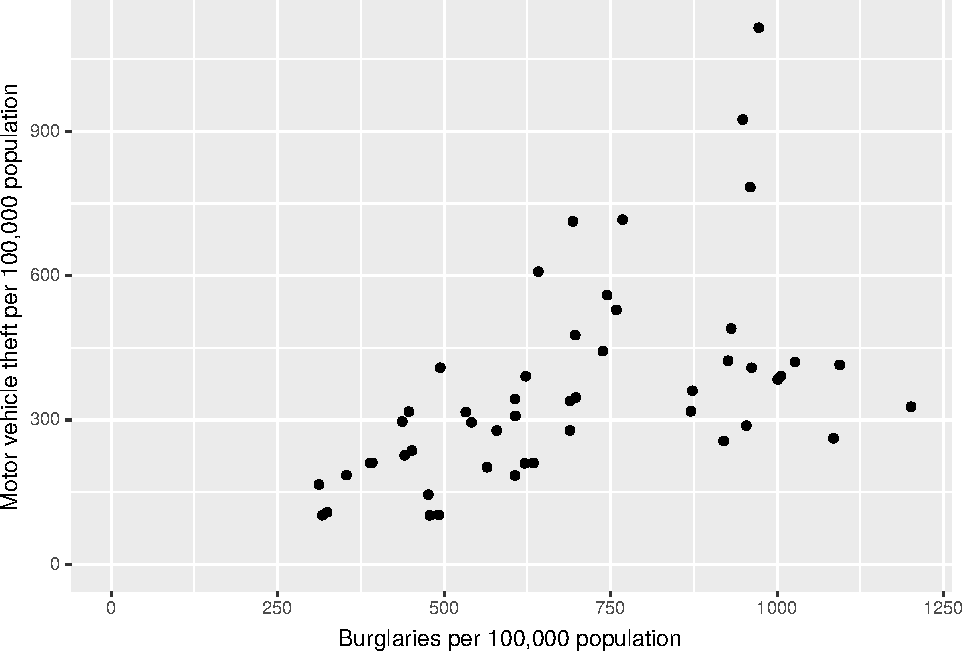
\includegraphics{bookdown-demo_files/figure-latex/unnamed-chunk-69-1.pdf}

\subsection{Bar Graphs}\label{bar-graphs}

As part of a study, elementary school students were asked which was more
important to them: good grades, popularity, or athletic ability. Here is
a brief look at the data.

\begin{Shaded}
\begin{Highlighting}[]
\OperatorTok{>}\StringTok{ }\NormalTok{u.goals <-}\StringTok{ "http://blue.for.msu.edu/FOR875/data/StudentGoals.csv"}
\OperatorTok{>}\StringTok{ }\NormalTok{StudentGoals <-}\StringTok{ }\KeywordTok{read.csv}\NormalTok{(u.goals, }\DataTypeTok{header =} \OtherTok{TRUE}\NormalTok{)}
\OperatorTok{>}\StringTok{ }\KeywordTok{head}\NormalTok{(StudentGoals)}
\end{Highlighting}
\end{Shaded}

\begin{verbatim}
  Gender Grade Age  Race  Type School   Goals Grades
1    boy     5  11 White Rural    Elm  Sports      1
2    boy     5  10 White Rural    Elm Popular      2
3   girl     5  11 White Rural    Elm Popular      4
4   girl     5  11 White Rural    Elm Popular      2
5   girl     5  10 White Rural    Elm Popular      4
6   girl     5  11 White Rural    Elm Popular      4
  Sports Looks Money
1      2     4     3
2      1     4     3
3      3     1     2
4      3     4     1
5      2     1     3
6      2     1     3
\end{verbatim}

First, a simple bar graph of the most important goal chosen is drawn,
followed by a stacked bar graph which also includes the student's
gender. We then add a side by side bar graph that includes the student's
gender.

\begin{Shaded}
\begin{Highlighting}[]
\KeywordTok{ggplot}\NormalTok{(StudentGoals, }\KeywordTok{aes}\NormalTok{(}\DataTypeTok{x =}\NormalTok{ Goals)) }\OperatorTok{+}\StringTok{ }\KeywordTok{geom_bar}\NormalTok{()}
\end{Highlighting}
\end{Shaded}

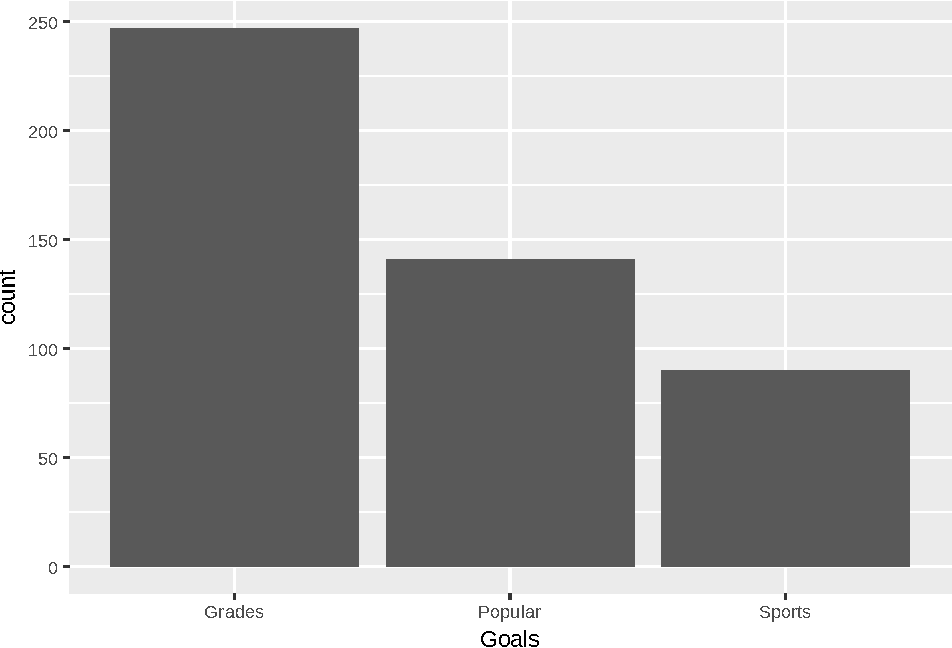
\includegraphics{bookdown-demo_files/figure-latex/unnamed-chunk-71-1.pdf}

\begin{Shaded}
\begin{Highlighting}[]
\KeywordTok{ggplot}\NormalTok{(StudentGoals, }\KeywordTok{aes}\NormalTok{(}\DataTypeTok{x =}\NormalTok{ Goals, }\DataTypeTok{fill =}\NormalTok{ Gender)) }\OperatorTok{+}\StringTok{ }\KeywordTok{geom_bar}\NormalTok{()}
\end{Highlighting}
\end{Shaded}

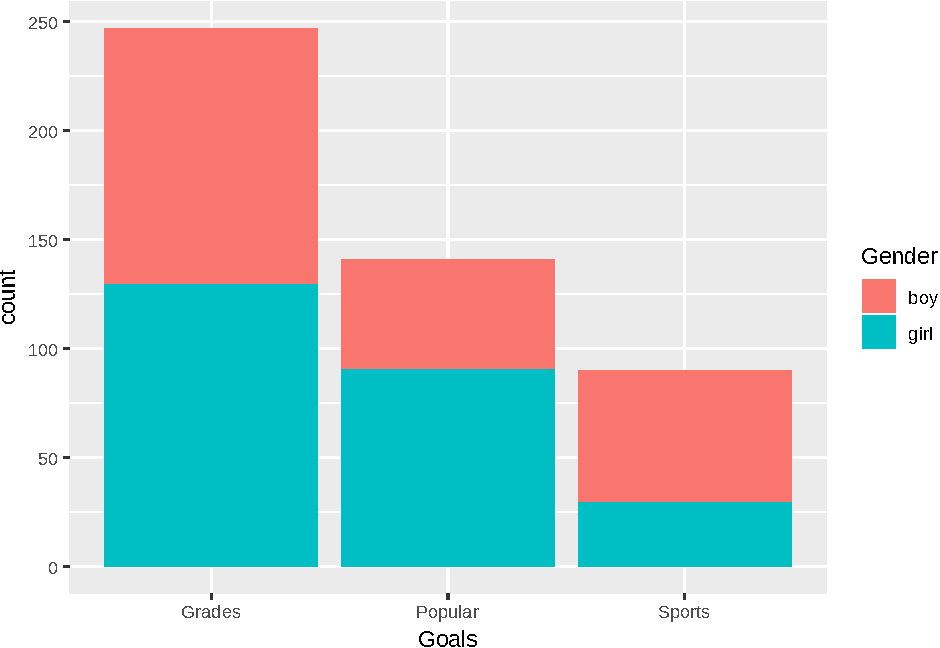
\includegraphics{bookdown-demo_files/figure-latex/unnamed-chunk-71-2.pdf}

\begin{Shaded}
\begin{Highlighting}[]
\KeywordTok{ggplot}\NormalTok{(StudentGoals, }\KeywordTok{aes}\NormalTok{(}\DataTypeTok{x =}\NormalTok{ Goals, }\DataTypeTok{fill =}\NormalTok{ Gender)) }\OperatorTok{+}\StringTok{ }
\StringTok{    }\KeywordTok{geom_bar}\NormalTok{(}\DataTypeTok{position =} \StringTok{"dodge"}\NormalTok{)}
\end{Highlighting}
\end{Shaded}

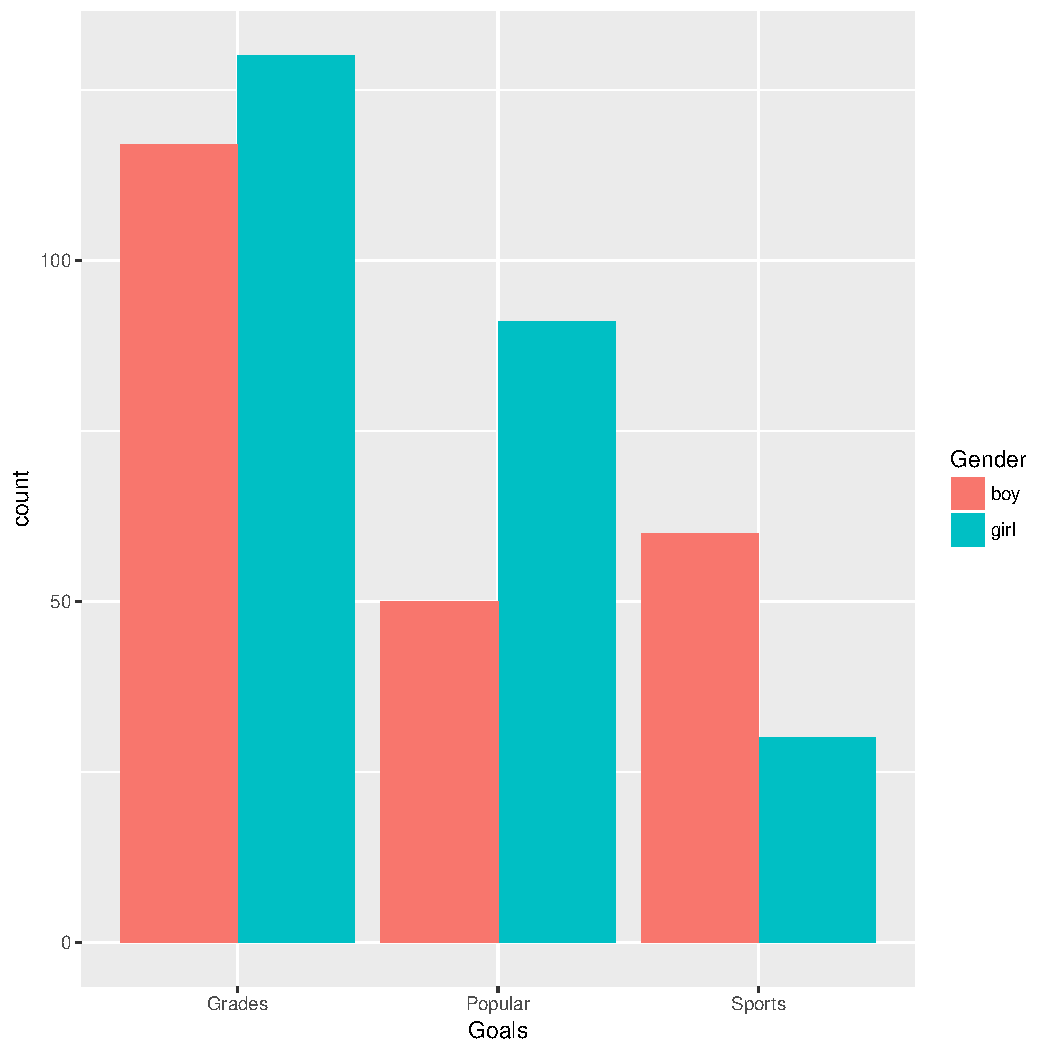
\includegraphics{bookdown-demo_files/figure-latex/unnamed-chunk-71-3.pdf}

In this example R counted the number of students who had each goal and
used these counts as the height of the bars. Sometimes the data contain
the bar heights as a variable. For example, we create a bar graph of
India's per capita GDP with separate bars for each year in the
data\footnote{R offers a large color palette, run \texttt{colors()} on
  the console to see a list of color names.}.

\begin{Shaded}
\begin{Highlighting}[]
\KeywordTok{ggplot}\NormalTok{(}\KeywordTok{subset}\NormalTok{(gapminder, country }\OperatorTok{==}\StringTok{ "India"}\NormalTok{), }\KeywordTok{aes}\NormalTok{(}\DataTypeTok{x =}\NormalTok{ year, }\DataTypeTok{y =}\NormalTok{ gdpPercap)) }\OperatorTok{+}\StringTok{ }
\StringTok{    }\KeywordTok{geom_bar}\NormalTok{(}\DataTypeTok{stat =} \StringTok{"identity"}\NormalTok{, }\DataTypeTok{color =} \StringTok{"black"}\NormalTok{, }\DataTypeTok{fill =} \StringTok{"steelblue2"}\NormalTok{) }\OperatorTok{+}\StringTok{ }
\StringTok{    }\KeywordTok{ggtitle}\NormalTok{(}\StringTok{"India's per-capita GDP"}\NormalTok{)}
\end{Highlighting}
\end{Shaded}

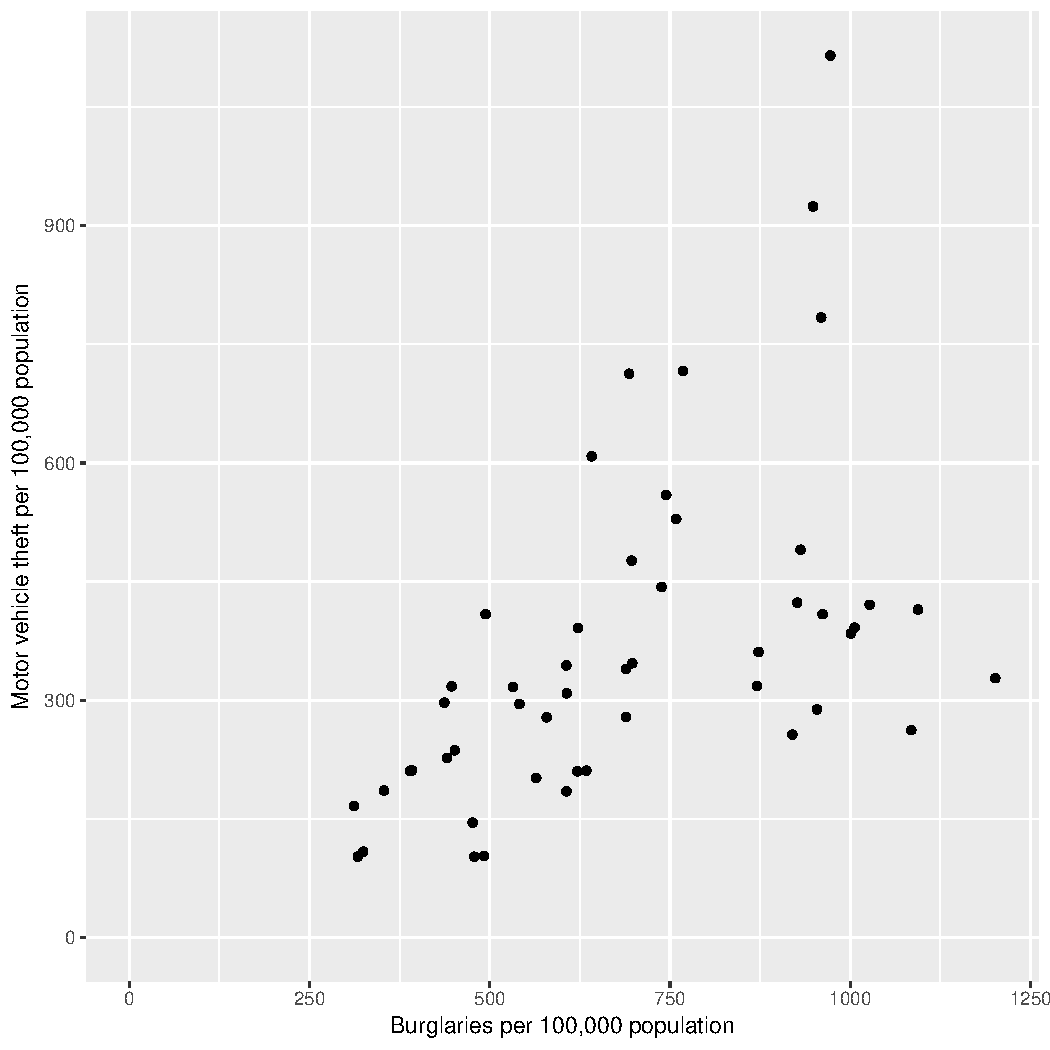
\includegraphics{bookdown-demo_files/figure-latex/unnamed-chunk-72-1.pdf}

\subsection{Graphs of Functions}\label{graphs-of-functions}

One way to create a plot of a mathematical function \(f\) is to create a
data frame with \(x\) values in one column and \(f(x)\) values in
another column, and then draw a line plot.

\begin{Shaded}
\begin{Highlighting}[]
\NormalTok{x <-}\StringTok{ }\KeywordTok{seq}\NormalTok{(}\OperatorTok{-}\NormalTok{pi, pi, }\DataTypeTok{len =} \DecValTok{1000}\NormalTok{)}
\NormalTok{sin.data <-}\StringTok{ }\KeywordTok{data.frame}\NormalTok{(}\DataTypeTok{x =}\NormalTok{ x, }\DataTypeTok{y =} \KeywordTok{sin}\NormalTok{(x))}
\KeywordTok{ggplot}\NormalTok{(}\DataTypeTok{data =}\NormalTok{ sin.data, }\KeywordTok{aes}\NormalTok{(}\DataTypeTok{x =}\NormalTok{ x, }\DataTypeTok{y =}\NormalTok{ y)) }\OperatorTok{+}\StringTok{ }\KeywordTok{geom_line}\NormalTok{() }\OperatorTok{+}\StringTok{ }
\StringTok{    }\KeywordTok{scale_y_continuous}\NormalTok{(}\DataTypeTok{name =} \StringTok{"sin(x)"}\NormalTok{)}
\end{Highlighting}
\end{Shaded}

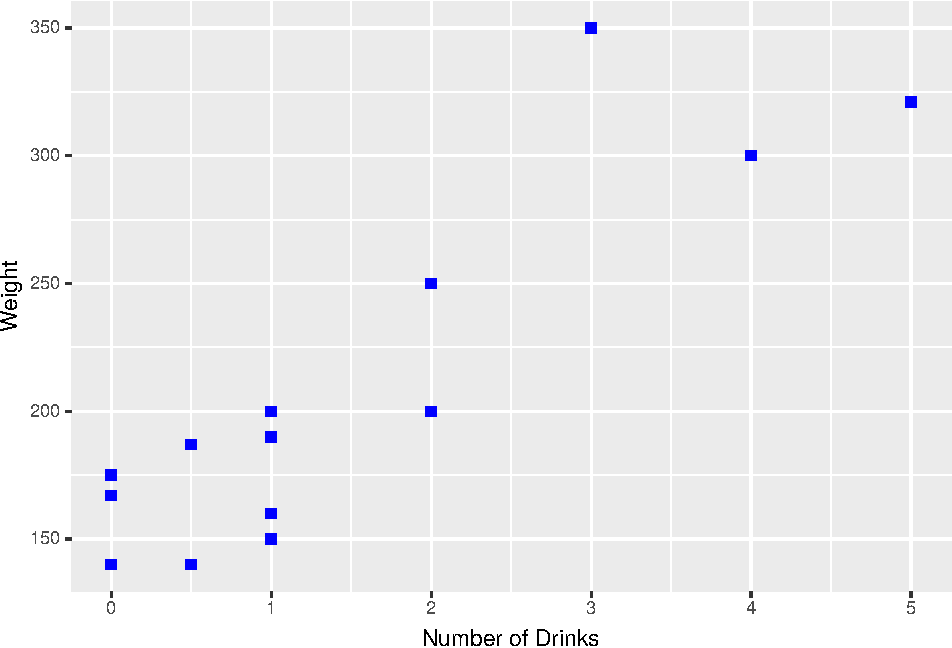
\includegraphics{bookdown-demo_files/figure-latex/unnamed-chunk-73-1.pdf}

This method works well, but with a better understanding of functions in
R we will be able to plot mathematical functions in a simpler and more
natural way.

\section{Themes}\label{themes}

The theme defines non-data aspects of the plot's characteristics such as
background color, axes, and grid lines. Default themes include:
\texttt{theme\_bw()}, \texttt{theme\_classic()}, \texttt{theme\_dark()},
\texttt{theme\_gray()}, \texttt{theme\_light()},
\texttt{theme\_linedraw()}, \texttt{theme\_minimal()}, and
\texttt{theme\_void()}. Changing the theme is as easy as adding it to
your initial \texttt{ggplot()} call. Here I replace the default implicit
\texttt{theme\_bw()} theme with the classic theme.

\begin{Shaded}
\begin{Highlighting}[]
\KeywordTok{ggplot}\NormalTok{(}\DataTypeTok{data =}\NormalTok{ sin.data, }\KeywordTok{aes}\NormalTok{(}\DataTypeTok{x =}\NormalTok{ x, }\DataTypeTok{y =}\NormalTok{ y)) }\OperatorTok{+}\StringTok{ }\KeywordTok{geom_line}\NormalTok{() }\OperatorTok{+}\StringTok{ }
\StringTok{    }\KeywordTok{scale_y_continuous}\NormalTok{(}\DataTypeTok{name =} \StringTok{"sin(x)"}\NormalTok{) }\OperatorTok{+}
\StringTok{    }\KeywordTok{theme_classic}\NormalTok{()}
\end{Highlighting}
\end{Shaded}

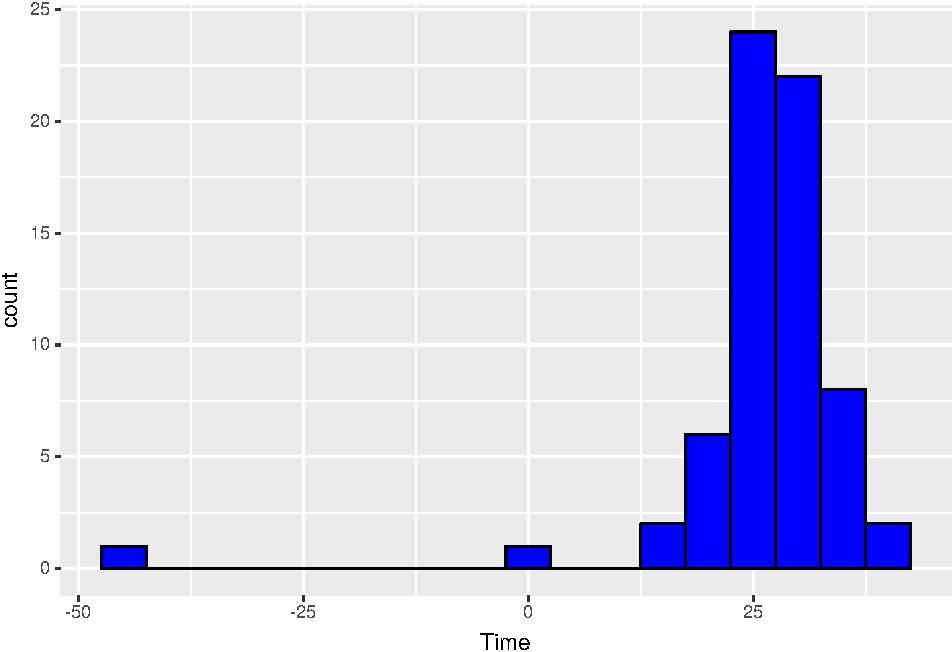
\includegraphics{bookdown-demo_files/figure-latex/unnamed-chunk-74-1.pdf}

The \texttt{ggthemes} add-on package
{[}\url{https://github.com/jrnold/ggthemes}{]} by Jeffrey Arnold
provides a large selection of themes beyond the eight themes that come
with \texttt{ggplot2}.

\section{Saving graphics}

We often want to export our graphics to use in an external document or
share with colleagues. There are several ways to save graphics in a
variety of file formats. The \verb+ggsave()+ function will allow you to
save your most recent \verb+ggplot()+ to a variety of vector (e.g.,
\texttt{eps\textquotesingle{}\textquotesingle{},}ps'`,
\texttt{pdf\textquotesingle{}\textquotesingle{},}svg'`) or raster (e.g.,
\texttt{jpeg\textquotesingle{}\textquotesingle{},}tiff'`,
\texttt{png\textquotesingle{}\textquotesingle{},}bmp'`,
\texttt{wmf\textquotesingle{}\textquotesingle{})\ formats\textbackslash{}footnote\{Vector\ files\ comprise\ lines\ and\ curves\ known\ as\ paths,\ whereas\ raster\ files\ are\ comprised\ of\ pixels.\ Vector\ images\ are\ often\ preferred\ for\ publication\ quality\ graphics\ because\ they\ can\ be\ edited,\ scale\ well,\ and\ provide\ crisper\ detail.\}.\ The\ subsequent\ call\ to\ \textbackslash{}verb+ggsave()+\ saves\ the\ \textbackslash{}verb+sin.data+\ plot\ to\ a\ pdf\ file\ called}sin-plot.pdf''.
\textless{}\textgreater{}= ggplot(filename = ``sin-plot.pdf'',
device=``pdf'') @ The \verb+ggplot()+ function takes additional
arguments to control scale, measurement units, and raster plot
resolution, i.e., dots per inch (dpi).

\section{More Resources}\label{more-resources}

In summary, \texttt{ggplot2} provides a fairly intuitive\footnote{Like
  everything else in this book, it takes practice to get used to the
  syntax.} framework for developing an enormous variety of graphics. In
addition to the resources mentioned at the beginning of this chapter,
there are numerous online \texttt{ggplot2} resources and galleries to
get ideas for creating beautiful graphics to convey the stories in your
data. See, for example,

\begin{itemize}
\tightlist
\item
  \url{http://docs.ggplot2.org}
\item
  \url{http://www.r-graph-gallery.com/portfolio/ggplot2-package}
\item
  \url{http://www.ggplot2-exts.org/gallery}
\item
  \url{http://www.cookbook-r.com/Graphs}
\item
  and of course www.google.com
\end{itemize}

While the built-in \texttt{ggplot2} package documentation (accessible
via the help tab in RStudio) is helpful, the official online
documentation at \url{http://docs.ggplot2.org} is particularly useful
because it provides example plots and easy navigation between related
topics. The large number number of functions and syntax in
\texttt{ggplot2} can be daunting. RStudio provides some handy
cheatsheets to help you along www.rstudio.com/resources/cheatsheets or
direct link
www.rstudio.com/wp-content/uploads/2016/11/ggplot2-cheatsheet-2.1.pdf.

\texttt{ggplot2} also has an active mailing list at
\url{http://groups.google.com/group/ggplot2}. The list is an excellent
resource for users at all stages of experience. Another useful resource
is stackoverflow, \url{http://stackoverflow.com}. There is an active
\texttt{ggplot2} community on stackoverflow, and many common questions
have already been asked and answered. When posting questions on any
programming mailing list, it is best to provide a minimal reproducible
example of your issue. The \texttt{reprex}
\url{https://github.com/jennybc/reprex} package by Jenny Bryan provides
a convenient way to do this, and also includes advice on creating a good
example. The more information you provide about your issue, the more
likely the community is to help you.

\section{Practice Exercises}\label{practice-exercises-2}

\section{Homework}\label{homework-2}

\textbf{Exercise 6} Learning objectives: practice using \texttt{ggplot2}
functions; summarize variables using graphics; introduce
\texttt{ggplot2} facets.

\bibliography{book.bib,packages.bib}


\end{document}
